\documentclass[mathserif]{beamer}
\usepackage{beamerthemeshadow}
\usepackage{beamerthemesplit}
%\usetheme{shadow}
\usecolortheme{default}
\setbeamertemplate{footline}[frame number]
\useinnertheme[shadow=true]{rounded}
%\setbeamertemplate{footline}{\insertframenumber/\inserttotalframenumber}
%\useoutertheme{infolines}
%\setbeamertemplate{headline}{} % removes the headline that infolines inserts

%\usetheme{boxes}
%\usepackage{amsmass}
%\usepackage{amssymb,amsfonts,url}

\usepackage{algorithm}
\usepackage{algorithmic}

\usepackage{graphicx}
\graphicspath{{Problems/}}
\usepackage{caption}
\captionsetup[figure]{labelformat=simple}
\captionsetup[table]{labelformat=simple}


\usepackage{tikz}
\usetikzlibrary{shadows}
\usetikzlibrary{positioning}
\usepackage{verbatim}
\usepackage{pgfplots}
\usepackage{verbatim}
\usetikzlibrary{arrows,shapes}

\definecolor{darkblue}{rgb}{0.2,0.2,0.6}
\definecolor{darkred}{rgb}{0.6,0.1,0.1}
\definecolor{darkgreen}{rgb}{0.2,0.6,0.2}

\usetikzlibrary{shadings,shadows,shapes.arrows}

\usetikzlibrary{calc} 
\makeatletter 
\@namedef{color@3}{blue!20}
\@namedef{color@1}{green!70}   
%\@namedef{color@3}{yellow!50} 
\@namedef{color@2}{orange!90}  
%\@namedef{color@5}{magenta!70} 
%\@namedef{color@6}{yellow!70}    

\newcommand{\graphitemize}[2]{%
\begin{tikzpicture}[every node/.style={align=center}, scale=0.78]  
 \draw[fill=green!5, fill opacity=0.1, green, inner sep=0.05cm, outer sep=0.05cm] (5,0) arc(0:360:5);
 % \draw[fill=white,draw=white, fill opacity=0.1, white, inner sep=0.05cm, outer sep=0.05cm] (4,0) arc(0:360:4);
%  \shade[ball color=gray!10!] (0,0) coordinate(Hp) circle (.9);
  \node[shape=circle,  minimum size=1.1cm,fill=red!60,font=\Large,outer sep =.15cm,inner sep=.2cm,drop  shadow={ashadow, color=red!60!black}](ce){#1};  
   % \shade[ball color=blue!20!] (0,0) coordinate($Algorithm$) circle (1.5cm);

\foreach \gritem [count=\xi] in {#2}  {\global\let\maxgritem\xi}  
\foreach \gritem [count=\xi] in {#2}
{% 
\pgfmathtruncatemacro{\angle}{90+360/\maxgritem*\xi}
\edef\col{\@nameuse{color@\xi}}
\node[shape=circle,
     ultra thick,
     draw=white,
     fill opacity=1,
     drop  shadow={ashadow, color=blue!60},
     fill=\col,outer sep=0.25cm,        
     minimum size=2cm] (satellite-\xi) at (\angle:5cm) {\gritem };
     \draw[line width=0.25cm,-latex, \col] (ce) -- (satellite-\xi);
     }%
% \draw[violet, fill=violet!10] (4,0) arc(0:360:4);
\end{tikzpicture}  
}%



\newcommand*{\tikzarrow}[2]{%
  \tikz[
    baseline=(A.base),             % Set baseline to the baseline of node content
    font=\footnotesize\sffamily    % Set fontsize of the node content
  ]
  \node[
    single arrow,                  % Shape of the node
    single arrow head extend=2pt,  % Actual width of arrow head
    draw,                          % Draw the node shape
    inner sep=2pt,                 % Separation between node content and node shape
    top color=white,               % Shading color on top of node
    bottom color=#1,               % Shading color on bottom of node
    drop shadow                    % Draw a shadow
  ] (A) {#2};%
}


\def\arrow{
  (10.05:1.1) -- (6.05:1) arc (6.05:120:1) [rounded corners=0.5] --
  (120:0.9) [rounded corners=1] -- (130:1.1) [rounded corners=0.5] --
  (120:1.3) [sharp corners] -- (120:1.2) arc (120:5.25:1.2)
  [rounded corners=1] -- (10.05:1.1) -- (6.05:1) -- cycle
}

\tikzset{
  ashadow/.style={opacity=.25, shadow xshift=0.07, shadow yshift=-0.07},
}

\def\arrows[#1]{         
  \begin{scope}[scale=#1]
    \draw[color=darkred, drop  shadow={ashadow, color=red!60!black}] \arrow;

    \draw[color=darkgreen, bottom color=green!90!black, top color=green!60,   drop shadow={ashadow, color=green!60!black}] [rotate=120] \arrow;

    \draw[color=darkblue, right color=blue, left color=blue!60,   drop shadow={ashadow, color=blue!60!black}] [rotate=240] \arrow;

    % to hide the green shadow
    \draw[color=darkred, left color=red, right color=red!60] \arrow;
  \end{scope}
}
\tikzstyle{vertex}=[circle,fill=black!25,draw,minimum size=20pt,inner sep=0pt]
\tikzstyle{middlevertex}=[circle,fill=black!25,draw,minimum size=15pt,inner sep=0pt]
\tikzstyle{smallvertex}=[circle,fill=black!25,draw,minimum size=10pt,inner sep=0pt]
\tikzstyle{tinyvertex}=[circle,fill=black!25,draw,minimum size=6pt,inner sep=0pt]
\tikzstyle{selected vertex} = [vertex, draw,fill=red!24]
\tikzstyle{blue smallvertex} = [smallvertex, draw,fill=blue]
\tikzstyle{red smallvertex} = [smallvertex, draw,fill=red]
\tikzstyle{edge} = [draw,thick,->]
\tikzstyle{undirectededge} = [draw,thick]
\tikzstyle{weight} = [font=\small]
\tikzstyle{selected edge} = [draw,line width=3pt,-,red!50]
\tikzstyle{ignored edge} = [draw,line width=3pt,-,black!20]
\tikzstyle{squarednode}=[draw, fill=blue!20, thick, minimum size=5mm]
\tikzstyle{roundnode}=[circle, draw, fill=blue!20, thick, minimum size=5mm]



%\usepackage{CJK}
%\usepackage{pinyin}

%    \begin{figure}
%        \centering
%        \includegraphics[width=0.8\textwidth]{newGeneRep.eps}
%    \end{figure}

% \begin{figure}%
%   \begin{center}%
%     \begin{minipage}{0.70\textwidth}%
%      \includegraphics[width=1.0\textwidth]{comp25000.eps}%
%     \end{minipage}%
%     \begin{minipage}{0.30\textwidth}
%      \includegraphics[width=1.0\textwidth]{comparelabel.eps}%
%     \end{minipage}%
%   \end{center}
% \end{figure}

% \begin{table}
%   {\begin{tabular}{l|rrr}\line
%       & \multicolumn{3}{c}{Actual number of DCJ operations}\\
%       \# genes &\# genes $\times 1$&\# genes $\times 2$&\# genes  $\times 3$ \\
% \hline
%      (a)~25,000 & 0.5\% ~~&  0.9\% ~~& 1.7\%~~\\
%       (b)~10,000 & 0.8\%~~ &  1.4\% ~~& 2.7\%~~\\
%      (c)~ 1,000 & 2.7\%~~ & 4.7\%~~ & 14.7\%~~\\ \line
%     \end{tabular}} {}%
% \end{table}

% \begin{eqnarray}
% T(n) &=&  \sum_{i=1}^n C_i \\
%      &=&  \# PUSH + \#POP \\
%      &<& 2\times \#PUSH \\
%      &<& 2n \\
% \end{eqnarray}

% \[ 
% \begin{matrix}
% \begin{pmatrix}
% C_{11} & C_{12} \\ 
% C_{21} & C_{22} 
% \end{pmatrix}
% =
% \begin{pmatrix}
% A_{11} & A_{12} \\ 
% A_{21} & A_{22}  
% \end{pmatrix}
% 
% \begin{pmatrix}
% B_{11} & B_{12} \\ 
% B_{21} & B_{22}  
%  
% \end{pmatrix}
%     
%    \end{matrix}
% \]
% 
% 
% \begin{eqnarray}
%  C_{11} &=& (A_{11}\times B_{11}) + (A_{12} \times B_{21}) \\
% C_{12} &=& (A_{11}\times B_{12}) + (A_{12} \times B_{22}) \\
% C_{21} &=& (A_{21}\times B_{11}) + (A_{22} \times B_{21}) \\
% C_{22} &=& (A_{21}\times B_{12}) + (A_{22} \times B_{22}) 
% \end{eqnarray}


\title{CS711008Z  Algorithm Design and Analysis }
\subtitle{ Lecture 7. Binary heap, binomial heap, and Fibonacci heap 
%\footnote{The slides were made  based on Chapter 19, 20 of Introduction to algorithms, Data Structure by Ellis Horowitz, et al,  a note by Danny Sleator, and the slides by Kevin Wayne with permission.} 
}
\author{Dongbo Bu} 
\institute{ {\small Institute of Computing Technology \\ 
Chinese Academy of Sciences, Beijing, China}}

\date{}

\begin{document}
%\begin{CJK}{UTF8}{cyberbit}

\frame{\titlepage}

\frame{
\frametitle{Outline}
\begin{itemize}
\item Introduction to priority queue  
\item Various implementations of priority queue:
\begin{itemize}
\item Linked list: a list having $n$ items is too long to support efficient {\sc ExtractMin} and {\sc Insert} operations simultaneously; 
\item Binary heap: using a \textcolor{red}{\bf tree} rather than a \textcolor{red}{\bf linked list};  
\item Binomial heap:  allowing  \textcolor{red}{\bf multiple trees } rather than \textcolor{red}{\bf a single tree} to  support efficient {\sc Union} operation
\item Fibonacci heap: implement {\sc DecreaseKey} via simply \textcolor{red}{\bf cutting an edge} rather than \textcolor{red}{\bf exchanging nodes}, and control  a ``bushy" tree shape via allowing \textcolor{red}{\bf at most one child losing} for any node. 

\end{itemize}
\end{itemize}
}

\frame{
	\begin{block}{}
		Priority queue
	\end{block}
}

\frame{
	\frametitle{ Priority queue: motivation } 
	\begin{itemize}
		\item Motivation: It is usually a case to \textcolor{red}{\bf extract the minimum} from a set $S$ of $n$ numbers, \textcolor{red}{\bf dynamically}. 
		\item Here, the word ``dynamically" means that on $S$, we might perform {\sc Insertion}, {\sc Deletion} and {\sc DecreaseKey} 
		operations.
		\item The question is how to organize the data to efficiently support these operations.  
	\end{itemize}
} 


\frame{
	\frametitle{ Priority queue } 

	\begin{itemize}
		\item {\bf Priority queue}  is an \textcolor{red}{\bf abstract data type} similar to stack or queue, but each {\bf element} has a {\bf priority} associated with its {\bf name}. 
		\item A min-oriented priority queue must  support the following core operations:  
			\begin{enumerate}
				\item $H$={\sc MakeHeap()}: to create a new heap $H$; 
				\item {\sc Insert}$(H, x)$:  to insert into $H$ an element $x$ together with its priority
				\item  {\sc ExtractMin}$(H)$:  to extract the element with the highest priority; 
				\item {\sc DecreaseKey}$(H, x, k)$: to decrease the priority of element $x$; 
%				\item {\sc FindMin}$(H)$: to find the element with the minimal priority; 
%				\item {\sc IsEmpty}$(H)$: return whether the priority queue is empty or not; 
%				\item {\sc Delete}$(H, x)$: to delete  element $x$ from $H$; 
				\item {\sc Union}$(H_1, H_2)$: return a new heap containing all elements of heaps $H_1$ and $H_2$, and destroy the input heaps
			\end{enumerate}
	\end{itemize}
}
\frame{
	\frametitle{Priority queue is very useful} 
		\begin{itemize}
		\item Priority queue has extensive applications, such as: 
			\begin{itemize}
				\item Dijkstra's shortest path algorithm
				\item Prim's MST algorithm
				\item Huffman coding
				\item $A^{*}$ searching algorithm
				\item HeapSort
				\item ......
			\end{itemize}
	\end{itemize}
}


\frame{
	\begin{block}{}
	An example: Dijkstra's algorithm
	\end{block}
}

\frame{
\frametitle{  Dijkstra's algorithm [1959] }


\begin{small}
{\sc Dijkstra}$( G, s, t )$
\begin{algorithmic}[1]
\STATE $key(s) = 0;$  //$key(u)$ stores an upper bound of the shortest distance from $s$ to $u$;
\STATE $PQ.$ {\sc Insert} $(s)$;
\FORALL{node $v \neq s$ }
	\STATE $key(v) = +\infty $
	\STATE $PQ.$ {\sc Insert} $(v)$ \textcolor{red}{//$n$ times}
\ENDFOR
\STATE $S=\{ \}$; // Let $S$ be the set of explored nodes;
\WHILE{$S \neq V $}
	\STATE $v^*=PQ.$ {\sc ExtractMin}$()$; \textcolor{red}{//$n$ times}
	\STATE $S=S \cup \{v^*\}$;
	\FORALL{$v \notin S$ and $<v^*, v> \in E$}
		\IF{$key(v^*) + d(v^*, v) < key(v)$}
			\STATE $PQ.${\sc DecreaseKey}($v, key(v^*) + d(v^*, v)$); \textcolor{red}{//$m$ times}
		\ENDIF
	\ENDFOR
\ENDWHILE
\end{algorithmic}
\end{small}
Here $PQ$ denotes a min-priority queue. 
}



\frame{
\frametitle{Dijkstra's algorithm: an example}

\begin{figure}
\begin{tikzpicture}[scale=0.86, auto,swap]

%problem 
     
    \foreach \pos/\name in {{(0,1)/s}, {(1.5,1)/a}, {(1.8, -0.8)/b}, {(0,-2.7)/c}, {(4.4 ,1)/d}, {(3.6,-2)/e}, {(5,-1.5)/f},{(6.5,-2.7)/t}}
        \node[middlevertex,fill=blue!20] (\name) at \pos {$\name$};
        
    \foreach \source/\dest/\weight in {s/a/9, s/b/14, s/c/15, a/d/24, b/d/18, b/e/30, c/e/20, d/e/2, e/f/11, e/t/16, f/t/6, d/t/19, c/t/44} 
                \draw[->, thick] (\source) -- node[above]{\small $\weight$} (\dest);
%initilization 

\end{tikzpicture} 
\end{figure}    
}


\frame{
\frametitle{Initialization}

\begin{figure}
\begin{tikzpicture}[scale=0.86, auto,swap]

    \foreach \pos/\name in {{(0,1)/s}, {(1.5,1)/a}, {(1.8, -0.8)/b}, {(0,-2.7)/c}, {(4.4 ,1)/d}, {(3.6,-2)/e}, {(5,-1.5)/f},{(6.5,-2.7)/t}}
        \node[middlevertex,fill=blue!20] (\name) at \pos {$\name$};
        
    \foreach \source/\dest/\weight in {s/a/9, s/b/14, s/c/15, a/d/24, b/d/18, b/e/30, c/e/20, d/e/2, e/f/11, e/t/16, f/t/6, d/t/19, c/t/44} 
                \draw[->, thick] (\source) -- node[above]{\small $\weight$} (\dest);
%initilization 


  \node[ultra thick, blue] at (3, 3) {$S=\{ \}$}; 
  \node[ultra thick, blue] at (3, 2.5) {$PQ=\{s(0), a(\infty), b(\infty), c(\infty), d(\infty), e(\infty), f(\infty), t(\infty)\}$}; 

\node[above, red] at (s.north) {$0$};
\node[above, red] at (a.north) {$\infty$};
\node[above, red] at (b.north) {$\infty$};
\node[above, red] at (c.north) {$\infty$};
\node[above, red] at (d.north) {$\infty$};
\node[above, red] at (e.north) {$\infty$};
\node[above, red] at (f.north) {$\infty$};   
\node[above, red] at  (t.north) {$\infty$};  

\end{tikzpicture} 
\end{figure}    
}


\frame{
\frametitle{Step 1: {\sc ExtractMin}}

\begin{figure}
\begin{tikzpicture}[scale=0.86, auto,swap]


    \foreach \pos/\name in {{(0,1)/s}, {(1.5,1)/a}, {(1.8, -0.8)/b}, {(0,-2.7)/c}, {(4.4 ,1)/d}, {(3.6,-2)/e}, {(5,-1.5)/f},{(6.5,-2.7)/t}}
        \node[middlevertex,fill=blue!20] (\name) at \pos {$\name$};
        
    \foreach \source/\dest/\weight in {s/a/9, s/b/14, s/c/15, a/d/24, b/d/18, b/e/30, c/e/20, d/e/2, e/f/11, e/t/16, f/t/6, d/t/19, c/t/44} 
                \draw[->, thick] (\source) -- node[above]{\small $\weight$} (\dest);
%initilization 


  \node[ultra thick, blue] at (3, 3) {$S=\{ \}$}; 
  \node[ultra thick, blue] at (3, 2.5) {$PQ=\{s(0), a(\infty), b(\infty), c(\infty), d(\infty), e(\infty), f(\infty), t(\infty)\}$}; 

\node[above, red] at (s.north) {$0$};
\node[above, red] at (a.north) {$\infty$};
\node[above, red] at (b.north) {$\infty$};
\node[above, red] at (c.north) {$\infty$};
\node[above, red] at (d.north) {$\infty$};
\node[above, red] at (e.north) {$\infty$};
\node[above, red] at (f.north) {$\infty$};   
\node[above, red] at  (t.north) {$\infty$};  


  \node[ ultra thick, green] at (8, 1) { {\sc ExtractMin} returns $s$}; 

\end{tikzpicture} 
\end{figure}    
}


\frame{
\frametitle{Step 1: {\sc DecreaseKey}}

\begin{figure}
\begin{tikzpicture}[scale=0.86, auto,swap]


%  \node[ultra thick, white] at (3, 3) {$S=\{ \}$}; 
%  \node[ultra thick, white] at (3, 2.5) {$PQ=\{s(0), a(\infty), b(\infty), c(\infty), d(\infty), e(\infty), f(\infty), t(\infty)\}$}; 

   \draw[fill=white,draw=white] (-2.7, 4) rectangle (10.5, -8); 
   
   \draw[fill=green, draw=green] (0,1.5) arc (90:450:0.5); 


    
    \foreach \pos/\name in {{(0,1)/s}, {(1.5,1)/a}, {(1.8, -0.8)/b}, {(0,-2.7)/c}, {(4.4 ,1)/d}, {(3.6,-2)/e}, {(5,-1.5)/f},{(6.5,-2.7)/t}}
        \node[middlevertex,fill=blue!20] (\name) at \pos {$\name$};

 
      
    \foreach \source/\dest/\weight in {s/a/9, s/b/14, s/c/15, a/d/24, b/d/18, b/e/30, c/e/20, d/e/2, e/f/11, e/t/16, f/t/6, d/t/19, c/t/44} 
                \draw[->, thick] (\source) -- node[above]{\small $\weight$} (\dest);

\node[above, red] at (s.north) {$0$};
\node[above, red] at (a.north) {$\infty$};
\node[above, red] at (b.north) {$\infty$};
\node[above, red] at (c.north) {$\infty$};
\node[above, red] at (d.north) {$\infty$};
\node[above, red] at (e.north) {$\infty$};
\node[above, red] at (f.north) {$\infty$};   
\node[above, red] at  (t.north) {$\infty$};  
 
  \node[ultra thick, blue] at (2, 3) {$S=\{ s \}$}; 
  \node[ultra thick, blue] at (2, 2.5) {$PQ=\{a(\infty), b(\infty), c(\infty), d(\infty), e(\infty), f(\infty), t(\infty) \}$}; 


  \node[ ultra thick, green] at (8, 0.5) { {\sc DecreaseKey}($a, 9$)}; 
  \node[ ultra thick, green] at (8,  0.0) { {\sc DecreaseKey}($b, 14$)}; 
  \node[ ultra thick, green] at (8, -0.5) { {\sc DecreaseKey}($c, 15$)}; 
  


\end{tikzpicture} 
\end{figure}    
}


\frame{
\frametitle{Step 2: {\sc ExtractMin}}

\begin{figure}
\begin{tikzpicture}[scale=0.86, auto,swap]

%s, a 
   \draw[fill=white,draw=white] (-2.7, 4) rectangle (10.5, -8); 
   
   \draw[fill=green, draw=green] (0,1.5) arc (90:450:0.5); 


    
    \foreach \pos/\name in {{(0,1)/s}, {(1.5,1)/a}, {(1.8, -0.8)/b}, {(0,-2.7)/c}, {(4.4 ,1)/d}, {(3.6,-2)/e}, {(5,-1.5)/f},{(6.5,-2.7)/t}}
        \node[middlevertex,fill=blue!20] (\name) at \pos {$\name$};

 
      
    \foreach \source/\dest/\weight in {s/a/9, s/b/14, s/c/15, a/d/24, b/d/18, b/e/30, c/e/20, d/e/2, e/f/11, e/t/16, f/t/6, d/t/19, c/t/44} 
                \draw[->, thick] (\source) -- node[above]{\small $\weight$} (\dest);

\node[above, red] at (s.north) {$0$};
\node[above, red] at (a.north) {$9$};
\node[above, red] at (b.north) {$14$};
\node[above, red] at (c.north) {$15$};
\node[above, red] at (d.north) {$\infty$};
\node[above, red] at (e.north) {$\infty$};
\node[above, red] at (f.north) {$\infty$};   
\node[above, red] at  (t.north) {$\infty$};  
 
  \node[ultra thick, blue] at (2, 3) {$S=\{ s \}$}; 
  \node[ultra thick, blue] at (2, 2.5) {$PQ=\{a(9), b(14), c(15), d(\infty), e(\infty), f(\infty), t(\infty) \}$}; 


\pause
  \node[ ultra thick, green] at (8, 1) { {\sc ExtractMin} returns $a$}; 



\end{tikzpicture} 
\end{figure}    
}


\frame{
\frametitle{Step 2: {\sc DecreaseKey}}

\begin{figure}
\begin{tikzpicture}[scale=0.86, auto,swap]


%\pause
%  \node[ultra thick, white] at (2, 3) {$S=\{ s \}$}; 
%  \node[ultra thick, white] at (2, 2.5) {$PQ=\{a(9), b(14), c(15), d(\infty), e(\infty), f(\infty), t(\infty) \}$}; 


  \draw[fill=white,draw=white] (-2.5, 3) rectangle (10.5, -8); 

  \def\d{2};
   \draw[fill=green, draw=green] (0,1.5) arc (90:180:0.5) -- (-0.5, 1 - \d + 0.5) arc (270:360:\d) -- (0,1.5); 
   
   
    \foreach \pos/\name in {{(0,1)/s}, {(1.5,1)/a}, {(1.8, -0.8)/b}, {(0,-2.7)/c}, {(4.4 ,1)/d}, {(3.6,-2)/e}, {(5,-1.5)/f},{(6.5,-2.7)/t}}
        \node[middlevertex,fill=blue!20] (\name) at \pos {$\name$};
        
    \foreach \source/\dest/\weight in {s/a/9, s/b/14, s/c/15, a/d/24, b/d/18, b/e/30, c/e/20, d/e/2, e/f/11, e/t/16, f/t/6, d/t/19, c/t/44} 
                \draw[->, thick] (\source) -- node[above]{\small $\weight$} (\dest);

\node[above, red] at (s.north) {$0$};
\node[above, red] at (a.north) {$9$};
\node[above, red] at (b.north) {$14$};
\node[above, red] at (c.north) {$15$};
\node[above, red] at (d.north) {$\infty$};
\node[above, red] at (e.north) {$\infty$};
\node[above, red] at (f.north) {$\infty$};   
\node[above, red] at  (t.north) {$\infty$};  
 
  \node[ultra thick, blue] at (2, 3) {$S=\{ s, a \}$}; 
  \node[ultra thick, blue] at (2, 2.5) {$PQ=\{ b(14), c(15), d(\infty), e(\infty), f(\infty), t(\infty) \}$}; 

\draw[->, line width=2pt, color=blue] (s) --  (a);

\node[ultra thick, green] at (8, 0.5) {{\sc DecreaseKey}($d, 33$)}; 
 


\end{tikzpicture} 
\end{figure}    
}


\frame{
\frametitle{Step 3: {\sc ExtractMin}}

\begin{figure}
\begin{tikzpicture}[scale=0.86, auto,swap]


 
%s, a

%  \node[ultra thick, white] at (2, 3) {$S=\{ s, a \}$}; 
%  \node[ultra thick, white] at (2, 2.5) {$PQ=\{ b(14), c(15), d(\infty), e(\infty), f(\infty), t(\infty) \}$}; 

   \draw[fill=white,draw=white] (-2.5, 3) rectangle (10.5, -8); 

  \def\d{2};
   \draw[fill=green, draw=green] (0,1.5) arc (90:180:0.5) -- (-0.5, 1 - \d + 0.5) arc (270:360:\d) -- (0,1.5); 
   
   
    \foreach \pos/\name in {{(0,1)/s}, {(1.5,1)/a}, {(1.8, -0.8)/b}, {(0,-2.7)/c}, {(4.4 ,1)/d}, {(3.6,-2)/e}, {(5,-1.5)/f},{(6.5,-2.7)/t}}
        \node[middlevertex,fill=blue!20] (\name) at \pos {$\name$};
        
    \foreach \source/\dest/\weight in {s/a/9, s/b/14, s/c/15, a/d/24, b/d/18, b/e/30, c/e/20, d/e/2, e/f/11, e/t/16, f/t/6, d/t/19, c/t/44} 
                \draw[->, thick] (\source) -- node[above]{\small $\weight$} (\dest);

\node[above, red] at (s.north) {$0$};
\node[above, red] at (a.north) {$9$};
\node[above, red] at (b.north) {$14$};
\node[above, red] at (c.north) {$15$};
\node[above, red] at (d.north) {$33$};
\node[above, red] at (e.north) {$\infty$};
\node[above, red] at (f.north) {$\infty$};   
\node[above, red] at  (t.north) {$\infty$};  
 
  \node[ultra thick, blue] at (2, 3) {$S=\{ s, a \}$}; 
  \node[ultra thick, blue] at (2, 2.5) {$PQ=\{ b(14), c(15), d(33), e(\infty), f(\infty), t(\infty) \}$}; 

\draw[->, line width=2pt, color=blue] (s) --  (a);


\pause
  \node[ ultra thick, green] at (8, 1) { {\sc ExtractMin} returns $b$}; 



\end{tikzpicture} 
\end{figure}    
}


\frame{
\frametitle{Step 3: {\sc DecreaseKey}}

\begin{figure}
\begin{tikzpicture}[scale=0.86, auto,swap]



%  \node[ultra thick, white] at (2, 3) {$S=\{ s, a \}$}; 
%  \node[ultra thick, white] at (2, 2.5) {$PQ=\{ b(14), c(15), d(33), e(\infty), f(\infty), t(\infty) \}$}; 
%
   \draw[fill=white,draw=white] (-2.5, 4) rectangle (10.5, -8); 

  \def\d{3.328};
   \draw[fill=green, draw=green] (0,1.5) arc (90:180:0.5) -- (-0.5, 1 - \d + 0.5) arc (270:360:\d) -- (0,1.5); 
    \foreach \pos/\name in {{(0,1)/s}, {(1.5,1)/a}, {(1.8, -0.8)/b}, {(0,-2.7)/c}, {(4.4 ,1)/d}, {(3.6,-2)/e}, {(5,-1.5)/f},{(6.5,-2.7)/t}}
        \node[middlevertex,fill=blue!20] (\name) at \pos {$\name$};
        
    \foreach \source/\dest/\weight in {s/a/9, s/b/14, s/c/15, a/d/24, b/d/18, b/e/30, c/e/20, d/e/2, e/f/11, e/t/16, f/t/6, d/t/19, c/t/44} 
                \draw[->, thick] (\source) -- node[above]{\small $\weight$} (\dest);


\node[above, red] at (s.north) {$0$};
\node[above, red] at (a.north) {$9$};
\node[above, red] at (b.north) {$14$};
\node[above, red] at (c.north) {$15$};
\node[above, red] at (d.north) {$33$};
\node[above, red] at (e.north) {$\infty$};
\node[above, red] at (f.north) {$\infty$};   
\node[above, red] at  (t.north) {$\infty$};  
 
  \node[ultra thick, blue] at (2, 3) {$S=\{ s, a, b \}$}; 
  \node[ultra thick, blue] at (2, 2.5) {$PQ=\{ c(15), d(33), e(\infty), f(\infty), t(\infty) \}$}; 

\draw[->, line width=2pt, color=blue] (s) --  (a);
\draw[->, line width=2pt, color=blue] (s) --  (b);

  \node[ ultra thick, green] at (8, 0.5) { {\sc DecreaseKey}($d, 32$)}; 
  \node[ ultra thick, green] at (8,  0.0) { {\sc DecreaseKey}($e, 44$)}; 

  

\end{tikzpicture} 
\end{figure}    
}


\frame{
\frametitle{Step 4: {\sc ExtractMin}}

\begin{figure}
\begin{tikzpicture}[scale=0.86, auto,swap]

%  \node[ultra thick, white] at (2, 3) {$S=\{ s, a, b \}$}; 
%  \node[ultra thick, white] at (2, 2.5) {$PQ=\{ c(15), d(33), e(\infty), f(\infty), t(\infty) \}$}; 

   \draw[fill=white,draw=white] (-2.5, 4) rectangle (10.5, -8); 

  \def\d{3.328};
   \draw[fill=green, draw=green] (0,1.5) arc (90:180:0.5) -- (-0.5, 1 - \d + 0.5) arc (270:360:\d) -- (0,1.5); 
    \foreach \pos/\name in {{(0,1)/s}, {(1.5,1)/a}, {(1.8, -0.8)/b}, {(0,-2.7)/c}, {(4.4 ,1)/d}, {(3.6,-2)/e}, {(5,-1.5)/f},{(6.5,-2.7)/t}}
        \node[middlevertex,fill=blue!20] (\name) at \pos {$\name$};
        
    \foreach \source/\dest/\weight in {s/a/9, s/b/14, s/c/15, a/d/24, b/d/18, b/e/30, c/e/20, d/e/2, e/f/11, e/t/16, f/t/6, d/t/19, c/t/44} 
                \draw[->, thick] (\source) -- node[above]{\small $\weight$} (\dest);


\node[above, red] at (s.north) {$0$};
\node[above, red] at (a.north) {$9$};
\node[above, red] at (b.north) {$14$};
\node[above, red] at (c.north) {$15$};
\node[above, red] at (d.north) {$32$};
\node[above, red] at (e.north) {$44$};
\node[above, red] at (f.north) {$\infty$};   
\node[above, red] at  (t.north) {$\infty$};  
 
  \node[ultra thick, blue] at (2, 3) {$S=\{ s, a, b \}$}; 
  \node[ultra thick, blue] at (2, 2.5) {$PQ=\{ c(15), d(32), e(44), f(\infty), t(\infty) \}$}; 

\draw[->, line width=2pt, color=blue] (s) --  (a);
\draw[->, line width=2pt, color=blue] (s) --  (b);



\pause
  \node[ ultra thick, green] at (8, 1) { {\sc ExtractMin} returns $c$}; 


\end{tikzpicture} 
\end{figure}    
}


\frame{
\frametitle{Step 4: {\sc DecreaseKey}}

\begin{figure}
\begin{tikzpicture}[scale=0.86, auto,swap]


%  \node[ultra thick, white] at (2, 3) {$S=\{ s, a, b \}$}; 
%  \node[ultra thick, white] at (2, 2.5) {$PQ=\{ c(15), d(32), e(44), f(\infty), t(\infty) \}$}; 

   \draw[fill=white,draw=white] (-2.5, 4) rectangle (10.5, -8); 

  \def\d{4.3};
   \draw[fill=green, draw=green] (0,1.5) arc (90:180:0.5) -- (-0.5, 1 - \d + 0.5) arc (270:360:\d) -- (0,1.5); 
    \foreach \pos/\name in {{(0,1)/s}, {(1.5,1)/a}, {(1.8, -0.8)/b}, {(0,-2.7)/c}, {(4.4 ,1)/d}, {(3.6,-2)/e}, {(5,-1.5)/f},{(6.5,-2.7)/t}}
        \node[middlevertex,fill=blue!20] (\name) at \pos {$\name$};
        
    \foreach \source/\dest/\weight in {s/a/9, s/b/14, s/c/15, a/d/24, b/d/18, b/e/30, c/e/20, d/e/2, e/f/11, e/t/16, f/t/6, d/t/19, c/t/44} 
                \draw[->, thick] (\source) -- node[above]{\small $\weight$} (\dest);
  
  
\node[above, red] at (s.north) {$0$};
\node[above, red] at (a.north) {$9$};
\node[above, red] at (b.north) {$14$};
\node[above, red] at (c.north) {$15$};
\node[above, red] at (d.north) {$32$};
\node[above, red] at (e.north) {$44$};
\node[above, red] at (f.north) {$\infty$};   
\node[above, red] at  (t.north) {$\infty$};  
 
  \node[ultra thick, blue] at (2, 3) {$S=\{ s, a, b, c \}$}; 
  \node[ultra thick, blue] at (2, 2.5) {$PQ=\{ d(32), e(44), f(\infty), t(\infty) \}$}; 

\draw[->, line width=2pt, color=blue] (s) --  (a);
\draw[->, line width=2pt, color=blue] (s) --  (b);
\draw[->, line width=2pt, color=blue] (s) --  (c);




  \node[ ultra thick, green] at (8, 0.5) { {\sc DecreaseKey}($e, 35$)}; 
  \node[ ultra thick, green] at (8,  0.0) { {\sc DecreaseKey}($t, 59$)}; 

  


\end{tikzpicture} 
\end{figure}    
}


\frame{
\frametitle{Step 5: {\sc ExtractMin}}

\begin{figure}
\begin{tikzpicture}[scale=0.86, auto,swap]



%  \node[ultra thick, white] at (2, 3) {$S=\{ s, a, b, c \}$}; 
%  \node[ultra thick, white] at (2, 2.5) {$PQ=\{ d(32), e(44), f(\infty), t(\infty) \}$}; 

   \draw[fill=white,draw=white] (-2.5, 4) rectangle (10.5, -8); 

  \def\d{4.3};
   \draw[fill=green, draw=green] (0,1.5) arc (90:180:0.5) -- (-0.5, 1 - \d + 0.5) arc (270:360:\d) -- (0,1.5); 
    \foreach \pos/\name in {{(0,1)/s}, {(1.5,1)/a}, {(1.8, -0.8)/b}, {(0,-2.7)/c}, {(4.4 ,1)/d}, {(3.6,-2)/e}, {(5,-1.5)/f},{(6.5,-2.7)/t}}
        \node[middlevertex,fill=blue!20] (\name) at \pos {$\name$};
        
    \foreach \source/\dest/\weight in {s/a/9, s/b/14, s/c/15, a/d/24, b/d/18, b/e/30, c/e/20, d/e/2, e/f/11, e/t/16, f/t/6, d/t/19, c/t/44} 
                \draw[->, thick] (\source) -- node[above]{\small $\weight$} (\dest);
  
  
\node[above, red] at (s.north) {$0$};
\node[above, red] at (a.north) {$9$};
\node[above, red] at (b.north) {$14$};
\node[above, red] at (c.north) {$15$};
\node[above, red] at (d.north) {$32$};
\node[above, red] at (e.north) {$35$};
\node[above, red] at (f.north) {$\infty$};   
\node[above, red] at  (t.north) {$59$};  
 
  \node[ultra thick, blue] at (2, 3) {$S=\{ s, a, b, c \}$}; 
  \node[ultra thick, blue] at (2, 2.5) {$PQ=\{  d(32), e(35), t(59), f(\infty) \}$}; 

\draw[->, line width=2pt, color=blue] (s) --  (a);
\draw[->, line width=2pt, color=blue] (s) --  (b);
\draw[->, line width=2pt, color=blue] (s) --  (c);
   


\pause
  \node[ ultra thick, green] at (8, 1) { {\sc ExtractMin} returns $d$}; 



\end{tikzpicture} 
\end{figure}    
}


\frame{
\frametitle{Step 5: {\sc DecreaseKey}}

\begin{figure}
\begin{tikzpicture}[scale=0.86, auto,swap]


 
%  \node[ultra thick, white] at (2, 3) {$S=\{ s, a, b, c \}$}; 
%  \node[ultra thick, white] at (2, 2.5) {$PQ=\{  d(32), e(35), t(59), f(\infty) \}$}; 

   \draw[fill=white,draw=white] (-2.5, 4) rectangle (10.5, -8); 

  \def\d{4.8};
   \draw[fill=green, draw=green] (0,1.5) arc (90:180:0.5) -- (-0.5, 1 - \d + 0.5) arc (270:360:\d) -- (0,1.5); 
    \foreach \pos/\name in {{(0,1)/s}, {(1.5,1)/a}, {(1.8, -0.8)/b}, {(0,-2.7)/c}, {(4.4 ,1)/d}, {(3.6,-2)/e}, {(5,-1.5)/f},{(6.5,-2.7)/t}}
        \node[middlevertex,fill=blue!20] (\name) at \pos {$\name$};
        
    \foreach \source/\dest/\weight in {s/a/9, s/b/14, s/c/15, a/d/24, b/d/18, b/e/30, c/e/20, d/e/2, e/f/11, e/t/16, f/t/6, d/t/19, c/t/44} 
                \draw[->, thick] (\source) -- node[above]{\small $\weight$} (\dest);
 
 
   
\node[above, red] at (s.north) {$0$};
\node[above, red] at (a.north) {$9$};
\node[above, red] at (b.north) {$14$};
\node[above, red] at (c.north) {$15$};
\node[above, red] at (d.north) {$32$};
\node[above, red] at (e.north) {$35$};
\node[above, red] at (f.north) {$\infty$};   
\node[above, red] at  (t.north) {$59$};  
 
  \node[ultra thick, blue] at (2, 3) {$S=\{ s, a, b, c, d \}$}; 
  \node[ultra thick, blue] at (2, 2.5) {$PQ=\{  e(35), t(59), f(\infty) \}$}; 

\draw[->, line width=2pt, color=blue] (s) --  (a);
\draw[->, line width=2pt, color=blue] (s) --  (b);
\draw[->, line width=2pt, color=blue] (s) --  (c);
\draw[->, line width=2pt, color=blue] (b) --  (d);
   




  \node[ ultra thick, green] at (8, 0.5) { {\sc DecreaseKey}($t, 51$)}; 
  \node[ ultra thick, green] at (8,  0.0) { {\sc DecreaseKey}($e, 34$)}; 

  


\end{tikzpicture} 
\end{figure}    
}


\frame{
\frametitle{Step 6: {\sc ExtractMin}}

\begin{figure}
\begin{tikzpicture}[scale=0.86, auto,swap]


%   \node[ultra thick, white] at (2, 3) {$S=\{ s, a, b, c, d \}$}; 
%  \node[ultra thick, white] at (2, 2.5) {$PQ=\{  e(35), t(59), f(\infty) \}$}; 

 
   \draw[fill=white,draw=white] (-2.5, 4) rectangle (10.5, -8); 

  \def\d{4.8};
   \draw[fill=green, draw=green] (0,1.5) arc (90:180:0.5) -- (-0.5, 1 - \d + 0.5) arc (270:360:\d) -- (0,1.5); 
    \foreach \pos/\name in {{(0,1)/s}, {(1.5,1)/a}, {(1.8, -0.8)/b}, {(0,-2.7)/c}, {(4.4 ,1)/d}, {(3.6,-2)/e}, {(5,-1.5)/f},{(6.5,-2.7)/t}}
        \node[middlevertex,fill=blue!20] (\name) at \pos {$\name$};
        
    \foreach \source/\dest/\weight in {s/a/9, s/b/14, s/c/15, a/d/24, b/d/18, b/e/30, c/e/20, d/e/2, e/f/11, e/t/16, f/t/6, d/t/19, c/t/44} 
                \draw[->, thick] (\source) -- node[above]{\small $\weight$} (\dest);
 
 
   
\node[above, red] at (s.north) {$0$};
\node[above, red] at (a.north) {$9$};
\node[above, red] at (b.north) {$14$};
\node[above, red] at (c.north) {$15$};
\node[above, red] at (d.north) {$32$};
\node[above, red] at (e.north) {$34$};
\node[above, red] at (f.north) {$\infty$};   
\node[above, red] at  (t.north) {$51$};  
 
  \node[ultra thick, blue] at (2, 3) {$S=\{ s, a, b, c, d \}$}; 
  \node[ultra thick, blue] at (2, 2.5) {$PQ=\{  e(34), t(51), f(\infty) \}$}; 

\draw[->, line width=2pt, color=blue] (s) --  (a);
\draw[->, line width=2pt, color=blue] (s) --  (b);
\draw[->, line width=2pt, color=blue] (s) --  (c);
\draw[->, line width=2pt, color=blue] (b) --  (d);
   
\pause
  \node[ ultra thick, green] at (8, 1) { {\sc ExtractMin} returns $e$}; 


\end{tikzpicture} 
\end{figure}    
}


\frame{
\frametitle{Step 6: {\sc DecreaseKey}}

\begin{figure}
\begin{tikzpicture}[scale=0.86, auto,swap]


%  \node[ultra thick, white] at (2, 3) {$S=\{ s, a, b, c, d \}$}; 
%  \node[ultra thick, white] at (2, 2.5) {$PQ=\{  e(34), t(51), f(\infty) \}$}; 

   \draw[fill=white,draw=white] (-2.5, 4) rectangle (10.5, -8); 

  \def\d{5.5};
   \draw[fill=green, draw=green] (0,1.5) arc (90:180:0.5) -- (-0.5, 1 - \d + 0.5) arc (270:360:\d) -- (0,1.5); 
    \foreach \pos/\name in {{(0,1)/s}, {(1.5,1)/a}, {(1.8, -0.8)/b}, {(0,-2.7)/c}, {(4.4 ,1)/d}, {(3.6,-2)/e}, {(5,-1.5)/f},{(6.5,-2.7)/t}}
        \node[middlevertex,fill=blue!20] (\name) at \pos {$\name$};
        
    \foreach \source/\dest/\weight in {s/a/9, s/b/14, s/c/15, a/d/24, b/d/18, b/e/30, c/e/20, d/e/2, e/f/11, e/t/16, f/t/6, d/t/19, c/t/44} 
                \draw[->, thick] (\source) -- node[above]{\small $\weight$} (\dest);
   
    
\node[above, red] at (s.north) {$0$};
\node[above, red] at (a.north) {$9$};
\node[above, red] at (b.north) {$14$};
\node[above, red] at (c.north) {$15$};
\node[above, red] at (d.north) {$32$};
\node[above, red] at (e.north) {$34$};
\node[above, red] at (f.north) {$\infty$};   
\node[above, red] at  (t.north) {$51$};  

 
  \node[ultra thick, blue] at (2, 3) {$S=\{ s, a, b, c, d, e \}$}; 
  \node[ultra thick, blue] at (2, 2.5) {$PQ=\{ f(45),  t(50) \}$}; 

\draw[->, line width=2pt, color=blue] (s) --  (a);
\draw[->, line width=2pt, color=blue] (s) --  (b);
\draw[->, line width=2pt, color=blue] (s) --  (c);
\draw[->, line width=2pt, color=blue] (b) --  (d);
\draw[->, line width=2pt, color=blue] (d) --  (e);


  \node[ ultra thick, green] at (8, 0.5) { {\sc DecreaseKey}($f, 45$)}; 
  \node[ ultra thick, green] at (8,  0.0) { {\sc DecreaseKey}($t, 50$)}; 

  

   

\end{tikzpicture} 
\end{figure}    
}


\frame{
\frametitle{Step 7: {\sc ExtractMin}}

\begin{figure}
\begin{tikzpicture}[scale=0.86, auto,swap]



%   \node[ultra thick, white] at (2, 3) {$S=\{ s, a, b, c, d, e \}$}; 
%  \node[ultra thick, white] at (2, 2.5) {$PQ=\{ f(45),  t(50) \}$}; 

  
   \draw[fill=white,draw=white] (-2.5, 4) rectangle (10.5, -8); 

  \def\d{5.5};
   \draw[fill=green, draw=green] (0,1.5) arc (90:180:0.5) -- (-0.5, 1 - \d + 0.5) arc (270:360:\d) -- (0,1.5); 
    \foreach \pos/\name in {{(0,1)/s}, {(1.5,1)/a}, {(1.8, -0.8)/b}, {(0,-2.7)/c}, {(4.4 ,1)/d}, {(3.6,-2)/e}, {(5,-1.5)/f},{(6.5,-2.7)/t}}
        \node[middlevertex,fill=blue!20] (\name) at \pos {$\name$};
        
    \foreach \source/\dest/\weight in {s/a/9, s/b/14, s/c/15, a/d/24, b/d/18, b/e/30, c/e/20, d/e/2, e/f/11, e/t/16, f/t/6, d/t/19, c/t/44} 
                \draw[->, thick] (\source) -- node[above]{\small $\weight$} (\dest);
   
    
\node[above, red] at (s.north) {$0$};
\node[above, red] at (a.north) {$9$};
\node[above, red] at (b.north) {$14$};
\node[above, red] at (c.north) {$15$};
\node[above, red] at (d.north) {$32$};
\node[above, red] at (e.north) {$34$};
\node[above, red] at (f.north) {$45$};   
\node[above, red] at  (t.north) {$50$};  
 
  \node[ultra thick, blue] at (2, 3) {$S=\{ s, a, b, c, d, e \}$}; 
  \node[ultra thick, blue] at (2, 2.5) {$PQ=\{ f(45),  t(50) \}$}; 

\draw[->, line width=2pt, color=blue] (s) --  (a);
\draw[->, line width=2pt, color=blue] (s) --  (b);
\draw[->, line width=2pt, color=blue] (s) --  (c);
\draw[->, line width=2pt, color=blue] (b) --  (d);
\draw[->, line width=2pt, color=blue] (d) --  (e);
   

\pause
  \node[ ultra thick, green] at (8, 1) { {\sc ExtractMin} returns $f$}; 

  


\end{tikzpicture} 
\end{figure}    
}


\frame{
\frametitle{Step 7: {\sc DecreaseKey}}

\begin{figure}
\begin{tikzpicture}[scale=0.86, auto,swap]


  
%    \node[ultra thick, white] at (2, 3) {$S=\{ s, a, b, c, d, e \}$}; 
%  \node[ultra thick, white] at (2, 2.5) {$PQ=\{ f(45),  t(50) \}$}; 
  
   \draw[fill=white,draw=white] (-2.5, 4) rectangle (10.5, -8); 

  \def\d{6.3};
   \draw[fill=green, draw=green] (0,1.5) arc (90:180:0.5) -- (-0.5, 1 - \d + 0.5) arc (270:360:\d) -- (0,1.5); 
    \foreach \pos/\name in {{(0,1)/s}, {(1.5,1)/a}, {(1.8, -0.8)/b}, {(0,-2.7)/c}, {(4.4 ,1)/d}, {(3.6,-2)/e}, {(5,-1.5)/f},{(6.5,-2.7)/t}}
        \node[middlevertex,fill=blue!20] (\name) at \pos {$\name$};
        
    \foreach \source/\dest/\weight in {s/a/9, s/b/14, s/c/15, a/d/24, b/d/18, b/e/30, c/e/20, d/e/2, e/f/11, e/t/16, f/t/6, d/t/19, c/t/44} 
                \draw[->, thick] (\source) -- node[above]{\small $\weight$} (\dest);
 
     
\node[above, red] at (s.north) {$0$};
\node[above, red] at (a.north) {$9$};
\node[above, red] at (b.north) {$14$};
\node[above, red] at (c.north) {$15$};
\node[above, red] at (d.north) {$32$};
\node[above, red] at (e.north) {$34$};
\node[above, red] at (f.north) {$45$};   
\node[above, red] at  (t.north) {$50$};  
 
  \node[ultra thick, blue] at (2, 3) {$S=\{ s, a, b, c, d, e, f \}$}; 
  \node[ultra thick, blue] at (2, 2.5) {$PQ=\{   t(50) \}$}; 

\draw[->, line width=2pt, color=blue] (s) --  (a);
\draw[->, line width=2pt, color=blue] (s) --  (b);
\draw[->, line width=2pt, color=blue] (s) --  (c);
\draw[->, line width=2pt, color=blue] (b) --  (d);
\draw[->, line width=2pt, color=blue] (d) --  (e);
\draw[->, line width=2pt, color=blue] (e) --  (f);   


 
   

\end{tikzpicture} 
\end{figure}    
}


\frame{
\frametitle{Step 8: {\sc ExtractMin}}

\begin{figure}
\begin{tikzpicture}[scale=0.86, auto,swap]


  
%    \node[ultra thick, white] at (2, 3) {$S=\{ s, a, b, c, d, e, f \}$}; 
%  \node[ultra thick, white] at (2, 2.5) {$PQ=\{   t(50) \}$}; 

   \draw[fill=white,draw=white] (-2.5, 4) rectangle (10.5, -8); 

  \def\d{8};
   \draw[fill=green, draw=green] (0,1.5) arc (90:180:0.5) -- (-0.5, 1 - \d + 0.5) arc (270:360:\d) -- (0,1.5); 
    \foreach \pos/\name in {{(0,1)/s}, {(1.5,1)/a}, {(1.8, -0.8)/b}, {(0,-2.7)/c}, {(4.4 ,1)/d}, {(3.6,-2)/e}, {(5,-1.5)/f},{(6.5,-2.7)/t}}
        \node[middlevertex,fill=blue!20] (\name) at \pos {$\name$};
        
    \foreach \source/\dest/\weight in {s/a/9, s/b/14, s/c/15, a/d/24, b/d/18, b/e/30, c/e/20, d/e/2, e/f/11, e/t/16, f/t/6, d/t/19, c/t/44} 
                \draw[->, thick] (\source) -- node[above]{\small $\weight$} (\dest);
   
 \node[above, red] at (s.north) {$0$};
\node[above, red] at (a.north) {$9$};
\node[above, red] at (b.north) {$14$};
\node[above, red] at (c.north) {$15$};
\node[above, red] at (d.north) {$32$};
\node[above, red] at (e.north) {$34$};
\node[above, red] at (f.north) {$45$};   
\node[above, red] at  (t.north) {$50$};  
 
  \node[ultra thick, blue] at (2, 3) {$S=\{ s, a, b, c, d, e, f, t \}$}; 
  \node[ultra thick, blue] at (2, 2.5) {$PQ=\{    \}$}; 

\draw[->, line width=2pt, color=blue] (s) --  (a);
\draw[->, line width=2pt, color=blue] (s) --  (b);
\draw[->, line width=2pt, color=blue] (s) --  (c);
\draw[->, line width=2pt, color=blue] (b) --  (d);
\draw[->, line width=2pt, color=blue] (d) --  (e);
\draw[->, line width=2pt, color=blue] (e) --  (f);   
\draw[->, line width=2pt, color=blue] (e) --  (t);   

          
   
\end{tikzpicture} 
\end{figure}    

}





\frame{
	\frametitle{ Time complexity of {\sc Dijkstra} algorithm} 

  \begin{table}
  \begin{tabular}{crrrr}
  \hline  \hline
  Operation & Linked  & Binary  & Binomial  & Fibonacci  \\
            &  list &  heap &  heap & heap \\
  \hline
  {\sc MakeHeap} & $ 1 $ &  $1$  & $ 1 $ & $1$  \\ 
  {\sc Insert} & $ 1 $ &  $\log n$  & $ \log n $ & $1$  \\ 
   {\sc ExtractMin} & $ n $ &  $\log n$  & $ \log n  $ & $ \log n $  \\ 
  {\sc DecreaseKey} & $ 1 $ &  $\log n$  & $ \log n $ & $1$  \\ 
  {\sc Delete} & $ n $ &  $\log n$  & $ \log n $ & $\log n$  \\ 
  {\sc Union} & $ 1 $ &  $ n $  & $ \log n $ & $1$  \\ 
   {\sc FindMin} & $ n $ &  $1$  & $ \log n $ & $1$  \\ 
  \hline 
  {\sc Dijkstra} & $ O(n^2) $ &  $ O(m \log n) $  & $ O( m \log n ) $ & $ O( m + n \log n) $  \\ 
  \hline \hline 
  \end{tabular} 
  \end{table}
{\sc Dijkstra} algorithm: $n$ {\sc Insert}, $n$ {\sc ExtractMin}, and $m$ {\sc DecreaseKey}. 
}

\frame{
	\begin{block}{}
	Implementing priority queue: array or linked list 
	\end{block}
}

\frame{
	\frametitle{Implementing priority queue: unsorted array} 
	\begin{itemize}
\item
	Unsorted array: 
\begin{figure}
    
\begin{tikzpicture}[scale=0.9, auto,swap]
  
  	\def\d{0.5};
	
 	\def\dy{3};
	\def\dx{-3};
    
       \foreach \i/\num/\name in { 0/8/s0,1/1/s1,2/6/s2,3/2/s3,4/4/s4, 5//s5, 6//s6, 7//s7} {
         	\draw[  thick ] (\i*\d + \dx,0+\dy) rectangle (\i*\d+\d + \dx, \d + \dy);
         	\node (\name) at (\i*\d+\d/2 + \dx, \d/2 + \dy) {$\num$};
   	 }
	
 
\end{tikzpicture}
\end{figure}

\item
 Unsorted linked list: 
\begin{figure}
    
\begin{tikzpicture}[scale=0.9, auto,swap]
  
  	\def\d{0.5};
	
 	\def\dy{3};
	\def\dx{-3};
 
        \foreach \i/\num/\name in { -1/head/head}{
         	\draw[  thick, white ] (\i*\d + \dx,0+\dy) rectangle (\i*\d+\d + \dx, \d + \dy);
         	\node[blue] (\name) at (\i*\d+\d/2 + \dx, -\i*\d + \d/2 + \dy) {$\num$};
   	 }
	    
       \foreach \i/\num/\name in { 0/8/s0,2/1/s2,4/6/s4,  6/2/s6,  8/4/s8} {
         	\draw[  thick ] (\i*\d + \dx,0+\dy) rectangle (\i*\d+\d + \dx, \d + \dy);
         	\node (\name) at (\i*\d+\d/2 + \dx, \d/2 + \dy) {$\num$};
   	 }
	\draw[->, thick, blue] (s0) -- (s2); 
	\draw[->, thick, blue] (s2) -- (s4); 
	\draw[->, thick, blue] (s4) -- (s6); 
	\draw[->, thick, blue] (s6) -- (s8); 
        

	 \draw[->, thick, blue] (head.south) to[in=180, out=270] (s0.west);
	 
\end{tikzpicture}
\end{figure}
	
\item Operations: 
	\begin{itemize}
		\item {\sc Insert}: $O(1)$
		\item {\sc ExtractMin}: $O(n)$
	\end{itemize} 
	\item Note: a list containing $n$ elements is too long to find the minimum efficiently. 
	\end{itemize} 
}

\frame{
	\frametitle{Implementing priority queue: sorted array}
	
	\begin{itemize}
\item
	Sorted array: 
\begin{figure}
    
\begin{tikzpicture}[scale=0.9, auto,swap]
  
  	\def\d{0.5};
	
 	\def\dy{3};
	\def\dx{-3};
    
       \foreach \i/\num/\name in { 0/1/s0,1/2/s1,2/4/s2,3/6/s3,4/8/s4, 5//s5, 6//s6, 7//s7} {
         	\draw[  thick ] (\i*\d + \dx,0+\dy) rectangle (\i*\d+\d + \dx, \d + \dy);
         	\node (\name) at (\i*\d+\d/2 + \dx, \d/2 + \dy) {$\num$};
   	 }
	
 
\end{tikzpicture}
\end{figure}

\item
 Sorted linked list: 
\begin{figure}
    
\begin{tikzpicture}[scale=0.9, auto,swap]
  
  	\def\d{0.5};
	
 	\def\dy{3};
	\def\dx{-3};
 
        \foreach \i/\num/\name in { -1/head/head}{
         	\draw[  thick, white ] (\i*\d + \dx,0+\dy) rectangle (\i*\d+\d + \dx, \d + \dy);
         	\node[blue] (\name) at (\i*\d+\d/2 + \dx, -\i*\d + \d/2 + \dy) {$\num$};
   	 }
	    
       \foreach \i/\num/\name in { 0/1/s0,2/2/s2,4/4/s4,  6/6/s6,  8/8/s8} {
         	\draw[  thick ] (\i*\d + \dx,0+\dy) rectangle (\i*\d+\d + \dx, \d + \dy);
         	\node (\name) at (\i*\d+\d/2 + \dx, \d/2 + \dy) {$\num$};
   	 }
	\draw[->, thick, blue] (s0) -- (s2); 
	\draw[->, thick, blue] (s2) -- (s4); 
	\draw[->, thick, blue] (s4) -- (s6); 
	\draw[->, thick, blue] (s6) -- (s8); 
        

	 \draw[->, thick, blue] (head.south) to[in=180, out=270] (s0.west);
	 
\end{tikzpicture}
\end{figure}
	
\item Operations: 
	\begin{itemize}
		\item {\sc Insert}: $O(n)$
		\item {\sc ExtractMin}: $O(1)$
	\end{itemize} 
		\item Note: a list containing $n$ elements is too long to maintain the order among elements. 
	\end{itemize} 
}





\frame{
	\frametitle{Implementing priority queue: array or linked list} 
%\begin{figure}
%	\begin{center}
%     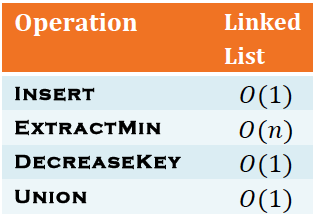
\includegraphics[width=1.5in]{L7-heaptablelinkedlist.png} 
%	\end{center}
%\end{figure}


\begin{table}[!ht]
\centering
\begin{tabular}{ p{2.4cm}p{1.1cm} }
\hline
 \textcolor{blue}{\textbf{Operation}} & \textcolor{blue}{\textbf{Linked List}}       \\
 \hline
 {\sc Insert} & $O(1)$        \\
 {\sc ExtractMin} & $O(n)$      \\
 {\sc DecreaseKey} & $O(1)$       \\
 {\sc Union} & $O(1)$   \\
 \hline
\end{tabular}
\end{table}


}



\frame{
	\begin{block}{}
	Binary heap: from \textcolor{red}{a linked list}  to \textcolor{red}{ a tree}
	%  (J. W. J. Williams, 1964, R. W. Floyd, 1964)
	\end{block}
} 

\frame{
\frametitle{Binary heap} 	
	\begin{figure}
		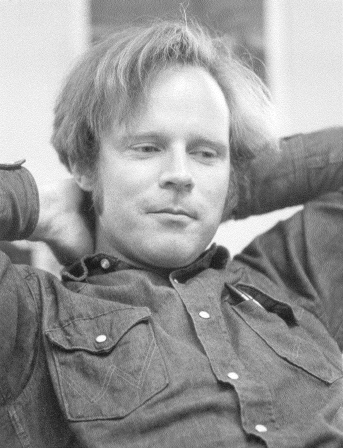
\includegraphics[width=1.5in]{Floyd.png}
		\caption{R. W. Floyd [1964]}
	\end{figure}
		
}

\frame{
	\frametitle{Binary heap: a complete binary tree}
	\begin{itemize}
	           \item Basic idea: 
	           	\begin{itemize}
			\item \textcolor{blue}{\bf loosing the structure}: Recall that the objective is to find the minimum. To achieve this objective, it is not necessary to sort all elements.
			\item \textcolor{blue}{\bf but don't loose it too much}: we still need order between some elements.
			\end{itemize}	
	\begin{figure}
\begin{tikzpicture}[scale=0.76, auto,swap]
    % Draw a 7,11 network
    % First we draw the vertices
    \foreach \pos/\name/\label in {{(0,0)/root/6}, {(-1,-1)/L/10}, {(1,-1)/R/8}, {(-1.5,-2)/LL/12}, {(-.5, -2)/LR/18}, {(0.5, -2)/RL/11}, {(1.5, -2)/RR/25}, {(-1.9, -3)/LLL/21}, {(-1.1, -3)/LLR/17}}
        \node[smallvertex,draw=black, fill=white!20] (\name) at \pos {\tiny $\label$};
  
    % Connect vertices with edges and draw weights
  \foreach \source/ \dest /\weight in {root/L/{}, root/R/{}, L/LL/{}, L/LR/{}, R/RL/{}, R/RR/{}, LL/LLL/{}, LL/LLR/{}}
        \path[undirectededge] (\source) -- node[weight] {$\weight$} (\dest);
%       \draw[dashed, ->] (0,0) arc  (120:60:2);

  \foreach \source/ \dest /\weight in {root/L/{},  L/LL/{},  LL/LLR/{}}
        \path[undirectededge, ultra thick, blue] (\source) -- node[weight] {$\weight$} (\dest);
%       \draw[dashed, ->] (0,0) arc  (120:60:2);
   \end{tikzpicture}
\end{figure}
	 \item Binary heap:   elements are stored in a \textcolor{red}{\bf complete binary tree}, i.e., a tree that is perfectly balanced except for the bottom level. \textcolor{red}{\bf Heap order} is required, i.e., any parent has a key smaller than his children;
	\item Advantage:   any path has a short length of $O(\log_2 n)$ rather than $n$ in linked list, making it efficient to maintain  heap order. 
	\end{itemize}
}


\frame{
	\frametitle{ Binary heap: an explicit implementation }
	
\begin{itemize}
	\item \textcolor{red}{\bf Pointer representation}: each node has pointers to its parent and two children; 
	\item The following information are maintained: 
		\begin{itemize}
			\item the number of elements $n$;
			\item the pointer to the root node; 
		\end{itemize}

\begin{figure}
\begin{tikzpicture}[scale=1., auto,swap]
    % Draw a 7,11 network
    % First we draw the vertices
    \foreach \pos/\name/\label in {{(0,0)/root/6}, {(-1,-1)/L/10}, {(1,-1)/R/8}, {(-1.5,-2)/LL/12}, {(-.5, -2)/LR/18}, {(0.5, -2)/RL/11}, {(1.5, -2)/RR/25}, {(-1.9, -3)/LLL/21}}
    %, {(-1.1, -3)/LLR/17}}
        \node[smallvertex,draw=black, fill=white!20] (\name) at \pos {\tiny $\label$};
  
   \node[blue, thick] at (-1, -0.5) {$lptr$}; 
   \node[blue, thick] at (1, -0.5) {$rptr$}; 
   
  \node[above, ultra thick, blue ] at (root.north) {$root$};
    % Connect vertices with edges and draw weights
  \foreach \source/ \dest /\weight in {root/L/{}, root/R/{}, L/LL/{}, L/LR/{}, R/RL/{}, R/RR/{}, LL/LLL/{}}
  %, LL/LLR/{}}
        \path[undirectededge] (\source) -- node[weight] {$\weight$} (\dest);
%       \draw[dashed, ->] (0,0) arc  (120:60:2);
   \end{tikzpicture}
\end{figure} 

	\item Note: the last node can be found in $O(\log n)$ time. 

\end{itemize}



}


\frame{
	\frametitle{ Binary heap: an implicit implementation }
	
\begin{itemize}
	\item \textcolor{red}{\bf Array representation}:  one-one correspondence between a binary tree and an array. 
	\begin{itemize}
	\item Binary tree $\Rightarrow$ array: 
		\begin{itemize}
			\item the indices starting  from $1$ for the sake of simplicity; 
			\item the indices record the order that 
		the binary tree is traversed  \textcolor{blue}{\bf level by level}.
		\end{itemize}

	\item Array $\Rightarrow$ binary tree: 
		\begin{itemize}
			\item the $k$-th item has two children located at $2k$ and $2k+1$; 
			\item the parent of the $k$-th item is  located at $\lfloor\frac{k}{2}\rfloor$; 
		\end{itemize}
	\end{itemize}
\begin{figure}
\begin{tikzpicture}[scale=1., auto,swap]
    % Draw a 7,11 network
    % First we draw the vertices
    \foreach \pos/\name/\label in {{(0,0)/root/6}, {(-1,-1)/L/10}, {(1,-1)/R/8}, {(-1.5,-2)/LL/12}, {(-.5, -2)/LR/18}, {(0.5, -2)/RL/11}, {(1.5, -2)/RR/25}, {(-1.9, -3)/LLL/21}}%, {(-1.1, -3)/LLR/17}}
        \node[smallvertex,draw=black, fill=white!20] (\name) at \pos {\tiny $\label$};
  
  \node[above, ultra thick, blue ] at (root.north) {\tiny $1$};
  \node[above, ultra thick, blue ] at (L.north) {\tiny $2$};
  \node[above, ultra thick, blue ] at (R.north) {\tiny $3$};
  \node[above, ultra thick, blue ] at (LL.north) {\tiny $4$};
  \node[above, ultra thick, blue ] at (LR.north) {\tiny $5$};
  \node[above, ultra thick, blue ] at (RL.north) {\tiny $6$};
   \node[above, ultra thick, blue ] at (RR.north) {\tiny $7$}; 
   \node[above, ultra thick, blue ] at (LLL.north) {\tiny $8$};
 %    \node[above, ultra thick, blue ] at (LLR.north) {\tiny $9$};
     
       
    % Connect vertices with edges and draw weights
  \foreach \source/ \dest /\weight in {root/L/{}, root/R/{}, L/LL/{}, L/LR/{}, R/RL/{}, R/RR/{}, LL/LLL/{}}%, LL/LLR/{}}
        \path[undirectededge] (\source) -- node[weight] {$\weight$} (\dest);
%       \draw[dashed, ->] (0,0) arc  (120:60:2);
 

         \node[ultra thick, red] at  (2, -1.3) {$\Leftrightarrow$};
  	\def\d{0.5};
 	\def\dy{-1.5};
	\def\dx{2.5};
    
       \foreach \i/\num/\name in { 0/6/s0,1/10/s1,2/8/s2,3/12/s3,4/18/s4, 5/11/s5, 6/25/s6, 7/21/s7, 8/\ /s8, 9/\ /s9, 10/\ /s10} {
         	\draw[  thick ] (\i*\d + \dx,0+\dy) rectangle (\i*\d+\d + \dx, \d + \dy);
         	\node (\name) at (\i*\d+\d/2 + \dx, \d/2 + \dy) {\tiny $\num$};
   	 }
     \node[below, ultra thick, blue ] at (s0.south) {\tiny $1$};
     \node[below, ultra thick, blue ] at (s1.south) {\tiny $2$};
     \node[below, ultra thick, blue ] at (s2.south) {\tiny $3$};
     \node[below, ultra thick, blue ] at (s3.south) {\tiny $4$};
      \node[below, ultra thick, blue ] at (s4.south) {\tiny $5$};
     \node[below, ultra thick, blue ] at (s5.south) {\tiny $6$};
     \node[below, ultra thick, blue ] at (s6.south) {\tiny $7$};
     \node[below, ultra thick, blue ] at (s7.south) {\tiny $8$};
     \node[below, ultra thick, blue ] at (s8.south) {\tiny $9$};
     \node[below, ultra thick, blue ] at (s9.south) {\tiny $10$};
     \node[below, ultra thick, blue ] at (s10.south) {\tiny $11$};
                                    
   \end{tikzpicture}

\end{figure} 


\end{itemize}



}


\frame{
	\frametitle{Sorted array vs. binary heap }

\begin{itemize}
	\item Sorted array: an array containing $n$ elements in an increasing order; 
	\begin{figure}
	\begin{tikzpicture} 
	
	\def\d{0.5};
 	\def\dy{-4.5};
	\def\dx{-2};
    
       \foreach \i/\num/\name in { 0/6/s0,1/8/s1,2/10/s2,3/11/s3,4/12/s4, 5/18/s5, 6/21/s6, 7/25/s7, 8/\ /s8, 9/\ /s9, 10/\ /s10} {
         	\draw[  thick ] (\i*\d + \dx,0+\dy) rectangle (\i*\d+\d + \dx, \d + \dy);
         	\node (\name) at (\i*\d+\d/2 + \dx, \d/2 + \dy) {\tiny $\num$};
   	 }
	 \draw[ thick, blue] (s0.north) to[out=90,in=90] (s1.north);
	 \draw[ thick, blue] (s1.north) to[out=90,in=90] (s2.north);
	 \draw[ thick, blue] (s2.north) to[out=90,in=90] (s3.north);
	 \draw[ thick, blue] (s3.north) to[out=90,in=90] (s4.north);
	 \draw[ thick, blue] (s4.north) to[out=90,in=90] (s5.north);
	 \draw[ thick, blue] (s5.north) to[out=90,in=90] (s6.north);
	 \draw[ thick, blue] (s6.north) to[out=90,in=90] (s7.north);

	 	 	 
     \node[below, ultra thick, blue ] at (s0.south) {\tiny $1$};
     \node[below, ultra thick, blue ] at (s1.south) {\tiny $2$};
     \node[below, ultra thick, blue ] at (s2.south) {\tiny $3$};
     \node[below, ultra thick, blue ] at (s3.south) {\tiny $4$};
      \node[below, ultra thick, blue ] at (s4.south) {\tiny $5$};
     \node[below, ultra thick, blue ] at (s5.south) {\tiny $6$};
     \node[below, ultra thick, blue ] at (s6.south) {\tiny $7$};
     \node[below, ultra thick, blue ] at (s7.south) {\tiny $8$};
     \node[below, ultra thick, blue ] at (s8.south) {\tiny $9$};
     \node[below, ultra thick, blue ] at (s9.south) {\tiny $10$};
     \node[below, ultra thick, blue ] at (s10.south) {\tiny $11$};
                                    
   \end{tikzpicture}

\end{figure} 
		
			
	
	\item Binary heap:  heap order means that only the order among nodes in short paths (length is less than $\log n$) are maintained. Note that some inverse pairs exist in the array. 
	
	
	
	\begin{figure}
	\begin{tikzpicture} 
	
	\def\d{0.5};
 	\def\dy{-4.5};
	\def\dx{-2};
    
       \foreach \i/\num/\name in { 0/6/s0,1/10/s1,2/8/s2,3/12/s3,4/18/s4, 5/11/s5, 6/25/s6, 7/21/s7, 8/\ /s8, 9/\ /s9, 10/\ /s10} {
         	\draw[  thick ] (\i*\d + \dx,0+\dy) rectangle (\i*\d+\d + \dx, \d + \dy);
         	\node (\name) at (\i*\d+\d/2 + \dx, \d/2 + \dy) {\tiny $\num$};
   	 }
	 \draw[ thick, blue] (s0.north) to[out=70,in=110] (s1.north);
	 \draw[ thick, blue] (s1.north) to[out=50,in=130] (s3.north);
	 \draw[ thick, blue] (s3.north) to[out=40,in=140] (s7.north);
	 	 	 
     \node[below, ultra thick, blue ] at (s0.south) {\tiny $1$};
     \node[below, ultra thick, blue ] at (s1.south) {\tiny $2$};
     \node[below, ultra thick, blue ] at (s2.south) {\tiny $3$};
     \node[below, ultra thick, blue ] at (s3.south) {\tiny $4$};
      \node[below, ultra thick, blue ] at (s4.south) {\tiny $5$};
     \node[below, ultra thick, blue ] at (s5.south) {\tiny $6$};
     \node[below, ultra thick, blue ] at (s6.south) {\tiny $7$};
     \node[below, ultra thick, blue ] at (s7.south) {\tiny $8$};
     \node[below, ultra thick, blue ] at (s8.south) {\tiny $9$};
     \node[below, ultra thick, blue ] at (s9.south) {\tiny $10$};
     \node[below, ultra thick, blue ] at (s10.south) {\tiny $11$};
                                    
   \end{tikzpicture}

\end{figure} 

\end{itemize}

}

\frame{

\begin{block}{}
Binary heap: primitive and other operations 
\end{block}
}


\frame{
	\frametitle{Primitive: exchanging nodes to restore heap order}
	\begin{itemize}
	\item Primitive operation: when heap order is violated, i.e. a parent has a value larger than only one of  its children, we simply exchange them to resolve the conflict. 
	
\begin{figure}
\begin{minipage}{0.45\textwidth}%
%	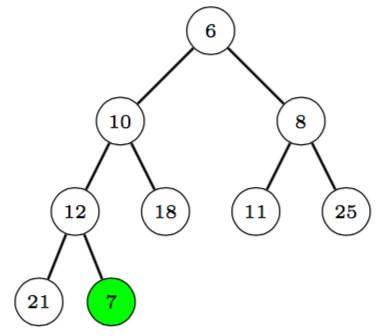
\includegraphics[width=\textwidth]{L7-binaryheapexample1.png}

\begin{tikzpicture}[auto,swap]

    \foreach \pos/\name/\label in {{(0,0)/root/6}, {(-1,-1)/L/10}, {(1,-1)/R/8}, {(-1.5,-2)/LL/18}, {(0.5, -2)/RL/11}, {(1.5, -2)/RR/25}, {(-1.9, -3)/LLL/21}}%, {(-1.1, -3)/LLR/7}}
        \node[smallvertex,draw=black, fill=white!20] (\name) at \pos {\tiny $\label$};
  
      \foreach \pos/\name/\label in {{(-1.1, -3)/LLR/27}}
        \node[smallvertex,draw=black, fill=white!20] (\name) at \pos {\tiny $\label$};

    \foreach \pos/\name/\label in { {(-1,-1)/L/15}}
        \node[smallvertex,draw=black, fill=green!20] (\name) at \pos {\tiny $\label$};

    \foreach \pos/\name/\label in { {(-.5, -2)/LR/13}}
        \node[smallvertex,draw=black, fill=red!20] (\name) at \pos {\tiny $\label$};
 
   \foreach \source/ \dest /\weight in {root/L/{}, root/R/{}, L/LL/{}, L/LR/{}, R/RL/{}, R/RR/{}, LL/LLL/{},  LL/LLR/{}}
        \path[undirectededge] (\source) -- node[weight] {$\weight$} (\dest);
    \end{tikzpicture}
\end{minipage}
\begin{minipage}{0.45\textwidth}
\begin{tikzpicture}[ auto,swap]

    \foreach \pos/\name/\label in {{(0,0)/root/6}, {(1,-1)/R/8},   {(-1.5,-2)/LL/18}, {(0.5, -2)/RL/11},  {(1.5, -2)/RR/25}, {(-1.9, -3)/LLL/21}, {(-1.1, -3)/LLR/27}}%, {(-1.1, -3)/LLR/7}}
        \node[smallvertex,draw=black, fill=white!20] (\name) at \pos {\tiny $\label$};
  
      \foreach \pos/\name/\label in {{(-1,-1)/L/13}}
        \node[smallvertex,draw=black, fill=red!20] (\name) at \pos {\tiny $\label$};
        
       \foreach \pos/\name/\label in {{(-.5, -2)/LR/15}}
        \node[smallvertex,draw=black, fill=green!20] (\name) at \pos {\tiny $\label$};    
 
   \foreach \source/ \dest /\weight in {root/L/{}, root/R/{}, L/LL/{}, L/LR/{}, R/RL/{}, R/RR/{}, LL/LLL/{},  LL/LLR/{}}
        \path[undirectededge] (\source) -- node[weight] {$\weight$} (\dest);

   \foreach \source/ \dest /\weight in {L/LL/{},  LL/LLR/{}}
        \path[undirectededge] (\source) -- node[weight] {$\weight$} (\dest);

    \end{tikzpicture}

    \end{minipage}
    \caption{Heap order is violated: $15 > 13$. Exchange  them to resolve the conflict. }
\end{figure} 
	\end{itemize}
} 	


\frame{
	\frametitle{Primitive: exchanging nodes to restore heap order}
	\begin{itemize}
	\item Primitive operation: when heap order is violated, i.e. a parent has a value larger than both of  its children, we exchange the parent with its smaller child to resolve the conflict. 
	

\begin{figure}
\begin{minipage}{0.45\textwidth}%
%	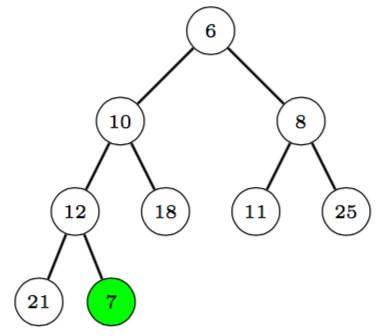
\includegraphics[width=\textwidth]{L7-binaryheapexample1.png}

\begin{tikzpicture}[auto,swap]

    \foreach \pos/\name/\label in {{(0,0)/root/6}, {(-1,-1)/L/10}, {(1,-1)/R/8}, {(0.5, -2)/RL/11}, {(1.5, -2)/RR/25}, {(-1.9, -3)/LLL/21}}%, {(-1.1, -3)/LLR/7}}
        \node[smallvertex,draw=black, fill=white!20] (\name) at \pos {\tiny $\label$};
  
      \foreach \pos/\name/\label in {{(-1.1, -3)/LLR/27}}
        \node[smallvertex,draw=black, fill=white!20] (\name) at \pos {\tiny $\label$};

    \foreach \pos/\name/\label in { {(-1.5,-2)/LL/12}, {(-.5, -2)/LR/18}}
        \node[smallvertex,draw=black, fill=red!20] (\name) at \pos {\tiny $\label$};

    \foreach \pos/\name/\label in { {(-1,-1)/L/20}}
        \node[smallvertex,draw=black, fill=green!20] (\name) at \pos {\tiny $\label$};

 
   \foreach \source/ \dest /\weight in {root/L/{}, root/R/{}, L/LL/{}, L/LR/{}, R/RL/{}, R/RR/{}, LL/LLL/{},  LL/LLR/{}}
        \path[undirectededge] (\source) -- node[weight] {$\weight$} (\dest);
    \end{tikzpicture}
\end{minipage}
\begin{minipage}{0.45\textwidth}
\begin{tikzpicture}[ auto,swap]

    \foreach \pos/\name/\label in {{(0,0)/root/6}, {(1,-1)/R/8}, {(0.5, -2)/RL/11}, {(1.5, -2)/RR/25}, {(-1.9, -3)/LLL/21}, {(-1.1, -3)/LLR/27}}%, {(-1.1, -3)/LLR/7}}
        \node[smallvertex,draw=black, fill=white!20] (\name) at \pos {\tiny $\label$};
  
      \foreach \pos/\name/\label in { {(-1.5,-2)/LL/20}}
        \node[smallvertex,draw=black, fill=green!20] (\name) at \pos {\tiny $\label$};
 

       \foreach \pos/\name/\label in {  {(-1,-1)/L/12}, {(-.5, -2)/LR/18}}
        \node[smallvertex,draw=black, fill=red!20] (\name) at \pos {\tiny $\label$};

   \foreach \source/ \dest /\weight in {root/L/{}, root/R/{}, L/LL/{}, L/LR/{}, R/RL/{}, R/RR/{}, LL/LLL/{},  LL/LLR/{}}
        \path[undirectededge] (\source) -- node[weight] {$\weight$} (\dest);

   \foreach \source/ \dest /\weight in {L/LL/{},  LL/LLR/{}}
        \path[undirectededge] (\source) -- node[weight] {$\weight$} (\dest);

    \end{tikzpicture}
    \end{minipage}
    \caption{Heap order is violated: $20 > 12$, and $20 > 18$. Exchange 20 with its smaller child (12) to resolve the conflicts. }
\end{figure} 
	\end{itemize}
} 	



\frame{
	\frametitle{Binary heap: {\sc Insert} operation }
	\begin{itemize}
	\item {\sc Insert} operation: the element is added as a  new node at  the end. Since the heap order might be violated, the node is repeatedly exchanged with its parent until heap order is restored. 
	\item For example, {\sc Insert( 7 )}: 

\begin{figure}
\begin{minipage}{0.45\textwidth}%
%	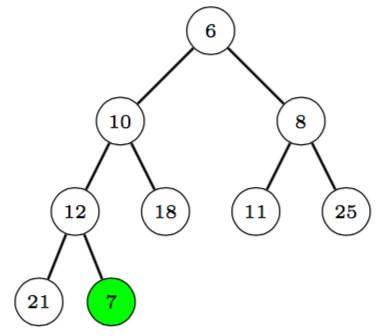
\includegraphics[width=\textwidth]{L7-binaryheapexample1.png}

\begin{tikzpicture}[auto,swap]

    \foreach \pos/\name/\label in {{(0,0)/root/6}, {(-1,-1)/L/10}, {(1,-1)/R/8}, {(-1.5,-2)/LL/12}, {(-.5, -2)/LR/18}, {(0.5, -2)/RL/11}, {(1.5, -2)/RR/25}, {(-1.9, -3)/LLL/21}}%, {(-1.1, -3)/LLR/7}}
        \node[smallvertex,draw=black, fill=white!20] (\name) at \pos {\tiny $\label$};
  
      \foreach \pos/\name/\label in {{(-1.1, -3)/LLR/7}}
        \node[smallvertex,draw=black, fill=green] (\name) at \pos {\tiny $\label$};
 
   \foreach \source/ \dest /\weight in {root/L/{}, root/R/{}, L/LL/{}, L/LR/{}, R/RL/{}, R/RR/{}, LL/LLL/{},  LL/LLR/{}}
        \path[undirectededge] (\source) -- node[weight] {$\weight$} (\dest);
    \end{tikzpicture}
\end{minipage}
\begin{minipage}{0.45\textwidth}
\begin{tikzpicture}[ auto,swap]

    \foreach \pos/\name/\label in {{(0,0)/root/6}, {(1,-1)/R/8},  {(-.5, -2)/LR/18}, {(0.5, -2)/RL/11}, {(1.5, -2)/RR/25}, {(-1.9, -3)/LLL/21}}%, {(-1.1, -3)/LLR/7}}
        \node[smallvertex,draw=black, fill=white!20] (\name) at \pos {\tiny $\label$};
  
      \foreach \pos/\name/\label in {{(-1,-1)/L/7}, {(-1.5,-2)/LL/10}, {(-1.1, -3)/LLR/12}}
        \node[smallvertex,draw=black, fill=green] (\name) at \pos {\tiny $\label$};
 
   \foreach \source/ \dest /\weight in {root/L/{}, root/R/{}, L/LL/{}, L/LR/{}, R/RL/{}, R/RR/{}, LL/LLL/{},  LL/LLR/{}}
        \path[undirectededge] (\source) -- node[weight] {$\weight$} (\dest);

   \foreach \source/ \dest /\weight in {L/LL/{},  LL/LLR/{}}
        \path[undirectededge, green] (\source) -- node[weight] {$\weight$} (\dest);

    \end{tikzpicture}
    \end{minipage}
\end{figure} 
	\end{itemize}
} 	


\frame{
	\frametitle{Binary heap: {\sc ExtractMin} operation }
	\begin{itemize}
	\item {\sc ExtractMin} operation: exchange element in root with the last node; repeatedly exchange the element in root with its \textcolor{blue}{\bf smaller child}  until heap order is restored. 
	\item For example, {\sc ExtractMin()}: 

\begin{figure}
\begin{minipage}{0.35\textwidth}%
\begin{tikzpicture}[auto,swap]
    \foreach \pos/\name/\label in { {(-1,-1)/L/10}, {(1,-1)/R/8}, {(-1.5,-2)/LL/12}, {(-.5, -2)/LR/18}, {(0.5, -2)/RL/11}, {(1.5, -2)/RR/25}} %, {(-1.9, -3)/LLL/21}}%, {(-1.1, -3)/LLR/7}}
        \node[smallvertex,draw=black, fill=white!20] (\name) at \pos {\tiny $\label$};
  
        \foreach \pos/\name/\label in {{(0,0)/root/6}}
        \node[smallvertex,draw=black,  fill=green!20] (\name) at \pos {\tiny $\label$};
  
      \foreach \pos/\name/\label in {{(-1.9, -3)/LLL/21}}
        \node[smallvertex,draw=black, fill=green!20] (\name) at \pos {\tiny $\label$};
 
   \foreach \source/ \dest /\weight in {root/L/{}, root/R/{}, L/LL/{}, L/LR/{}, R/RL/{}, R/RR/{}}
        \path[undirectededge] (\source) -- node[weight] {$\weight$} (\dest);
   \foreach \source/ \dest /\weight in { LL/LLL/{}}
        \path[undirectededge] (\source) -- node[weight] {$\weight$} (\dest);
                
    \end{tikzpicture}
\end{minipage}
\begin{minipage}{0.35\textwidth}%
\begin{tikzpicture}[auto,swap]
    \foreach \pos/\name/\label in {{(-1,-1)/L/10}, {(1,-1)/R/8}, {(-1.5,-2)/LL/12}, {(-.5, -2)/LR/18}, {(0.5, -2)/RL/11}, {(1.5, -2)/RR/25}} %, {(-1.9, -3)/LLL/21}}%, {(-1.1, -3)/LLR/7}}
        \node[smallvertex,draw=black, fill=white!20] (\name) at \pos {\tiny $\label$};
  
        \foreach \pos/\name/\label in { {(0,0)/root/21}}
        \node[smallvertex,draw=black,  fill=green] (\name) at \pos {\tiny $\label$};
  
      \foreach \pos/\name/\label in {{(-1.9, -3)/LLL/6}}
        \node[smallvertex,draw=black, dashed, fill=white!20] (\name) at \pos {\tiny $\label$};
 
   \foreach \source/ \dest /\weight in {root/L/{}, root/R/{}, L/LL/{}, L/LR/{}, R/RL/{}, R/RR/{}}
        \path[undirectededge] (\source) -- node[weight] {$\weight$} (\dest);
  
     \foreach \source/ \dest /\weight in { LL/LLL/{}}
        \path[undirectededge, dashed] (\source) -- node[weight] {$\weight$} (\dest);
        
    \end{tikzpicture}
\end{minipage}
\begin{minipage}{0.3\textwidth}
\begin{tikzpicture}[ auto,swap]

    \foreach \pos/\name/\label in {{(-1,-1)/L/10}, {(-1.5,-2)/LL/12}, {(-.5, -2)/LR/18}, {(1.5, -2)/RR/25}} 
        \node[smallvertex,draw=black, fill=white!20] (\name) at \pos {\tiny $\label$};
  
      \foreach \pos/\name/\label in {{(1,-1)/R/11}, {(0.5, -2)/RL/21}, {(0,0)/root/8}}
        \node[smallvertex,draw=black, fill=green] (\name) at \pos {\tiny $\label$};
 
   \foreach \source/ \dest /\weight in {root/L/{},L/LL/{}, L/LR/{},R/RR/{}}
        \path[undirectededge] (\source) -- node[weight] {$\weight$} (\dest);

   \foreach \source/ \dest /\weight in {root/R/{}, R/RL/{}}
        \path[undirectededge, green] (\source) -- node[weight] {$\weight$} (\dest);

    \end{tikzpicture}
    \end{minipage}
\end{figure} 
	\end{itemize}
} 	

\frame{
	\frametitle{Binary heap: {\sc DecreaseKey} operation }
	\begin{itemize}
	\item {\sc DecreaseKey} operation: given a handle to a node, repeatedly exchange the node with its parent until heap order is restored. 
	\item For example, {\sc DecreaseKey( $ptr$,  7 )}: 

\begin{figure}
\begin{minipage}{0.45\textwidth}%

\begin{tikzpicture}[auto,swap]
 
     \foreach \pos/\name/\label in {{(0,0)/root/6}, {(-1,-1)/L/10}, {(1,-1)/R/8}, {(-1.5,-2)/LL/12}, {(-.5, -2)/LR/18}, {(0.5, -2)/RL/11}, {(1.5, -2)/RR/25}, {(-1.9, -3)/LLL/21}}
        \node[smallvertex,draw=black, fill=white!20] (\name) at \pos {\tiny $\label$};
  
  \foreach \source/ \dest /\weight in {root/L/{}, root/R/{}, L/LL/{}, L/LR/{}, R/RL/{}, R/RR/{}, LL/LLL/{}}
        \path[undirectededge] (\source) -- node[weight] {$\weight$} (\dest);
 
 \node[ultra thick, blue] at (-0.9, -3) {$\leftarrow $ $ptr$};
 
   \end{tikzpicture}
\end{minipage}
\begin{minipage}{0.45\textwidth}
\begin{tikzpicture}[auto,swap]

     \foreach \pos/\name/\label in {{(0,0)/root/6},  {(1,-1)/R/8},  {(-.5, -2)/LR/18}, {(0.5, -2)/RL/11}, {(1.5, -2)/RR/25}}
        \node[smallvertex,draw=black, fill=white!20] (\name) at \pos {\tiny $\label$};
  
       \foreach \pos/\name/\label in {{(-1,-1)/L/7},  {(-1.5,-2)/LL/10}, {(-1.9, -3)/LLL/12}}
        \node[smallvertex,draw=black, fill=green] (\name) at \pos {\tiny $\label$};
        
  \foreach \source/ \dest /\weight in {root/L/{}, root/R/{}, L/LL/{}, L/LR/{}, R/RL/{}, R/RR/{}, LL/LLL/{}}
        \path[undirectededge] (\source) -- node[weight] {$\weight$} (\dest);
  
    \foreach \source/ \dest /\weight in {L/LL/{},  LL/LLL/{}}
        \path[undirectededge, ultra thick, green] (\source) -- node[weight] {$\weight$} (\dest);      
        
    \end{tikzpicture}
    \end{minipage}
\end{figure} 
	\end{itemize}
} 


\frame{
	\frametitle{Binary heap: analysis }
	\begin{theorem}
	In an \textcolor{red}{\bf implicit} binary heap, any sequence of $m$ {\sc Insert}, {\sc. DecreaseKey}, and {\sc ExtractMin} operations with $n$ {\sc Insert} operations takes $O(m \log n)$ time. 
	\end{theorem}	
		Note: 
		\begin{itemize}
			\item Each operation touches at most $\log n$ nodes on a path from the root to a leaf. 
		\end{itemize}
	
		\begin{theorem}
	In an \textcolor{red}{\bf explicit} binary heap with $n$ nodes, the {\sc Insert}, {\sc. DecreaseKey}, and {\sc ExtractMin} operations take $O(m \log n)$ time in the worst case.  
	\end{theorem}	
	Note: 
		\begin{itemize}
			\item If using array representation, a dynamic array expanding/contracting is needed. However, 
			 the total cost of array expanding/contracting  is $O(n)$ (see {\sc TableInsert}). 
		\end{itemize}
	
} 

\frame{
	\frametitle{Binary heap: heapify a set of items }
	\begin{itemize}
	\item Question: Given a set of $n$ elements, how to construct a binary heap containing them? 
	\item Solutions:
		\begin{enumerate}
		\item  Simply {\sc Insert} the elements one by one. Takes $O(n \log n)$ time. 
		\item Bottom-up heapifying. Takes $O(n)$ time. \\ For $i=n$ to $1$, we repeatedly exchange the element in node $i$ with its smaller child until the subtree rooted at node $i$ is heap-ordered. 
	 		\end{enumerate}

	\end{itemize}	
\begin{figure}
\begin{tikzpicture}[scale=0.9, auto,swap]
    % Draw a 7,11 network
    % First we draw the vertices
    \foreach \pos/\name/\label in {{(0,0)/root/21}, {(-1,-1)/L/10}, {(1,-1)/R/11}, {(-1.5,-2)/LL/25}, {(-.5, -2)/LR/8}, {(0.5, -2)/RL/18}, {(1.5, -2)/RR/12}, {(-1.9, -3)/LLL/6}}%, {(-1.1, -3)/LLR/17}}
        \node[smallvertex,draw=black, fill=white!20] (\name) at \pos {\tiny $\label$};
  
  \node[above, ultra thick, blue ] at (root.north) {\tiny $1$};
  \node[above, ultra thick, blue ] at (L.north) {\tiny $2$};
  \node[above, ultra thick, blue ] at (R.north) {\tiny $3$};
  \node[above, ultra thick, blue ] at (LL.north) {\tiny $4$};
  \node[above, ultra thick, blue ] at (LR.north) {\tiny $5$};
  \node[above, ultra thick, blue ] at (RL.north) {\tiny $6$};
   \node[above, ultra thick, blue ] at (RR.north) {\tiny $7$}; 
   \node[above, ultra thick, blue ] at (LLL.north) {\tiny $8$};
 %    \node[above, ultra thick, blue ] at (LLR.north) {\tiny $9$};
     
       
    % Connect vertices with edges and draw weights
  \foreach \source/ \dest /\weight in {root/L/{}, root/R/{}, L/LL/{}, L/LR/{}, R/RL/{}, R/RR/{}, LL/LLL/{}}%, LL/LLR/{}}
        \path[undirectededge] (\source) -- node[weight] {$\weight$} (\dest);
%       \draw[dashed, ->] (0,0) arc  (120:60:2);
 

  	\def\d{0.5};
 	\def\dy{-1};
	\def\dx{3};
    
       \foreach \i/\num/\name in { 0/21/s0,1/10/s1,2/11/s2,3/25/s3,4/8/s4, 5/18/s5, 6/12/s6, 7/6/s7, 8/\ /s8, 9/\ /s9, 10/\ /s10} {
         	\draw[  thick ] (\i*\d + \dx,0+\dy) rectangle (\i*\d+\d + \dx, \d + \dy);
         	\node (\name) at (\i*\d+\d/2 + \dx, \d/2 + \dy) {\tiny $\num$};
   	 }
     \node[below, ultra thick, blue ] at (s0.south) {\tiny $1$};
     \node[below, ultra thick, blue ] at (s1.south) {\tiny $2$};
     \node[below, ultra thick, blue ] at (s2.south) {\tiny $3$};
     \node[below, ultra thick, blue ] at (s3.south) {\tiny $4$};
      \node[below, ultra thick, blue ] at (s4.south) {\tiny $5$};
     \node[below, ultra thick, blue ] at (s5.south) {\tiny $6$};
     \node[below, ultra thick, blue ] at (s6.south) {\tiny $7$};
     \node[below, ultra thick, blue ] at (s7.south) {\tiny $8$};
     \node[below, ultra thick, blue ] at (s8.south) {\tiny $9$};
     \node[below, ultra thick, blue ] at (s9.south) {\tiny $10$};
     \node[below, ultra thick, blue ] at (s10.south) {\tiny $11$};
                                    
   \end{tikzpicture}

\end{figure} 
(see a demo)	
	
} 	


\frame{
	\frametitle{Binary heap: heapify} 
	\begin{theorem}
		Given $n$ elements, a binary heap can be constructed using $O(n)$ time. 
	\end{theorem}

	\begin{proof}
		\begin{itemize}
			\item There are at most $\lceil \frac{n}{2^{h+1}} \rceil$ nodes of height $h$; 
			\item It takes $O(h)$ time to sink a node of height $h$; 
			\item The total time is: 
			\begin{eqnarray}
			\sum_{h=0}^{\lfloor \log_2 n \rfloor} \lceil \frac{n}{2^{h+1}} \rceil h &\leq & \sum_{h=0}^{\lfloor \log_2 n \rfloor} n \frac{ h}{2^h} \nonumber  \\
			&\leq& 2n \nonumber
 			\end{eqnarray} 
		\end{itemize}
	\end{proof}	
} 	

	
\frame{
	\frametitle{Implementing priority queue: binary heap} 
%\begin{figure}
%	\begin{center}
%     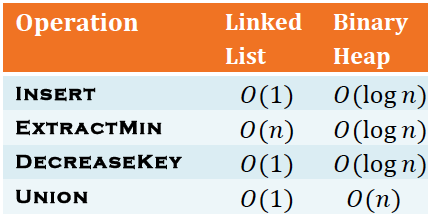
\includegraphics[width=2.5in]{L7-heaptablebinaryheap.png} 
%	\end{center}
%\end{figure}

\begin{table}[!ht]
\centering
\begin{tabular}{ p{2.4cm}p{1.1cm}p{1.3cm}  }
\hline
 \textcolor{blue}{\textbf{Operation}} & \textcolor{blue}{\textbf{Linked List}}  & \textcolor{blue}{\textbf{Binary Heap}}    \\
 \hline
 {\sc Insert} & $O(1)$ & $O(\log n)$       \\
 {\sc ExtractMin} & $O(n)$ & $O(\log n)$    \\
 {\sc DecreaseKey} & $O(1)$ & $O(\log n)$      \\
 {\sc Union} & $O(1)$ & $O(n)$     \\
 \hline
\end{tabular}
\end{table}

}



\frame{
	\frametitle{Binary heap: {\sc Union} operation }
	\begin{itemize}
	\item {\sc Union} operation: Given two binary heaps $H_1$ and $H_2$, to merge them into one binary heap. 
	
	\begin{figure}
\begin{tikzpicture}[scale=0.9, auto,swap]

    \foreach \pos/\name/\label in {{(0,0)/root/21}, {(-1,-1)/L/25}, {(1,-1)/R/27}, {(-1.5,-2)/LL/29}}
        \node[smallvertex,draw=black, fill=white!20] (\name) at \pos {\tiny $\label$};
    \foreach \source/ \dest /\weight in {root/L/{}, root/R/{}, L/LL/{}}
        \path[undirectededge] (\source) -- node[weight] {$\weight$} (\dest);
        
 \node[ultra thick, above, blue] at (root.north)  {$H_1$}; 

    \foreach \pos/\name/\label in {{(4+0,0)/root/6}, {(4-1,-1)/L/8}, {(4+1,-1)/R/11}}
        \node[smallvertex,draw=black, fill=white!20] (\name) at \pos {\tiny $\label$};
    \foreach \source/ \dest /\weight in {root/L/{}, root/R/{}}
        \path[undirectededge] (\source) -- node[weight] {$\weight$} (\dest);
        

 \node[ultra thick, above, blue] at (root.north)  {$H_2$}; 
 	

	
   \end{tikzpicture}

\end{figure} 
	
	\item $O(n)$ time is needed if using heapify. 
	\item Question: Is there a  quicker way to union two heaps? 
	
	\end{itemize}	
} 

	
\frame{
	\begin{block}{}
	Binomial heap: using  \textcolor{red}{multiple trees } rather than \textcolor{red}{a single tree} to support efficient {\sc Union} operation
	\end{block}
} 

\frame{
	\frametitle{Binomial heap} 	
\begin{figure}
     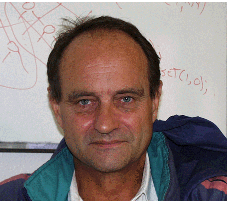
\includegraphics[width=1.5in]{JeanVuillemin.png}
 \caption{Jean Vuillenmin [1978]} 
\end{figure}
	
}


\frame{
	\frametitle{Binomial heap: efficient {\sc Union} } 

	\begin{itemize}
		\item Basic idea: 
		\begin{itemize}
			\item \textcolor{blue}{\bf loosing the structure}: if \textcolor{red}{\bf multiple trees} are allowed to  represent a heap,  {\sc Union} can be efficiently implemented via simply putting trees together. 
			\item \textcolor{blue}{\bf but don't loose it too much}: there should not be too many trees; otherwise, it will take a long time to find the minimum among all root nodes. 
		\end{itemize}
	\begin{figure}
\begin{tikzpicture}[scale=0.9, auto,swap]

    \foreach \pos/\name/\label in {{(0,0)/root/21}, {(-1,-1)/L/25}, {(1,-1)/R/27}, {(-1.5,-2)/LL/29}}
        \node[smallvertex,draw=black, fill=white!20] (\name) at \pos {\tiny $\label$};
    \foreach \source/ \dest /\weight in {root/L/{}, root/R/{}, L/LL/{}}
        \path[undirectededge] (\source) -- node[weight] {$\weight$} (\dest);
        
 \node[ultra thick, above, blue] at (root.north)  {$H_1$}; 

    \foreach \pos/\name/\label in {{(4+0,0)/root/6}, {(4-1,-1)/L/8}, {(4+1,-1)/R/11}}
        \node[smallvertex,draw=black, fill=white!20] (\name) at \pos {\tiny $\label$};
    \foreach \source/ \dest /\weight in {root/L/{}, root/R/{}}
        \path[undirectededge] (\source) -- node[weight] {$\weight$} (\dest);
        

 \node[ultra thick, above, blue] at (root.north)  {$H_2$}; 
 	

	
   \end{tikzpicture}
\end{figure} 
		
	\item {\sc ExtractMin}: simply finding the minimum element of the root nodes. Note that a root node holds the minimum of the tree due to the heap order. 
	\end{itemize}	
}

\frame{
	\frametitle{Why we can't loose the structure too much?} 
	\begin{itemize}
		\item An extreme case of multiple trees: each node is itself a tree. Then it will take $O(n)$ time to find the minimum. 

\begin{figure}
\begin{tikzpicture}[scale=0.9, auto,swap]




    \foreach \pos/\name/\label in {{(0,0)/root/6}, {(1,0)/L/11}, {(2,0)/R/8}, {(3,0)/LL/29}} 
        \node[smallvertex,draw=black, fill=white!20] (\name) at \pos {\tiny $\label$};

   \end{tikzpicture}
\end{figure} 
		
		\item Solution:  \textcolor{red}{\bf consolidating}, i.e., two trees (with the same size) are merged into one --- the larger root is linked to the smaller one to keep the heap order. Note that after consolidating,   at most $\log n$ trees will be left. 

\begin{figure}
\begin{tikzpicture}[scale=0.9, auto,swap]

   \def\dx{0};
   \def\dy{1.5};
    \foreach \pos/\name/\label in {{(0 +\dx,0 +\dy)/root/6}, {(1.5 + \dx, 0 + \dy)/L/11}} 
            \node[smallvertex,draw=black, fill=white!20] (\name) at \pos {\tiny $\label$};
   	


   \draw[->, line width=2pt, blue] (2, 2-0.5) -- node[above]{$link$} (3, 2-0.5); 
   \def\dx{3.5};
   \def\dy{2};
    \foreach \pos/\name/\label in {{(0 +\dx,0 +\dy)/root/6}, {(0 + \dx, -1 + \dy)/L/11}} 
            \node[smallvertex,draw=black, fill=white!20] (\name) at \pos {\tiny $\label$};
    \foreach \source/ \dest /\weight in {root/L/{}}
        \path[undirectededge] (\source) -- node[weight] {$\weight$} (\dest);



   \def\dx{0};
   \def\dy{0};
    \foreach \pos/\name/\label in {{(0 +\dx,0 +\dy)/root/6}, {(0 + \dx, -1 + \dy)/L/11}} 
            \node[smallvertex,draw=black, fill=white!20] (\name) at \pos {\tiny $\label$};
    \foreach \source/ \dest /\weight in {root/L/{}}
        \path[undirectededge] (\source) -- node[weight] {$\weight$} (\dest);


   \def\dx{1.5};
   \def\dy{0};
    \foreach \pos/\name/\label in {{(0 +\dx,0 +\dy)/root/8}, {(0 + \dx, -1 + \dy)/L/9}} 
            \node[smallvertex,draw=black, fill=white!20] (\name) at \pos {\tiny $\label$};
    \foreach \source/ \dest /\weight in {root/L/{}}
        \path[undirectededge] (\source) -- node[weight] {$\weight$} (\dest);

   \draw[->, line width=2pt, blue] (2, -0.5) -- node[above]{$link$} (3, -0.5); 
   

   \def\dx{3.5};
   \def\dy{0};
    \foreach \pos/\name/\label in {{(0 +\dx,0 +\dy)/root/6}, {(0 + \dx, -1 + \dy)/L/11}} 
            \node[smallvertex,draw=black, fill=white!20] (\name) at \pos {\tiny $\label$};
    \foreach \source/ \dest /\weight in {root/L/{}}
        \path[undirectededge] (\source) -- node[weight] {$\weight$} (\dest);


   \def\dx{4.5};
   \def\dy{-1};
    \foreach \pos/\name/\label in {{(0 +\dx,0 +\dy)/R/8}, {(0 + \dx, -1 + \dy)/RL/9}} 
            \node[smallvertex,draw=black, fill=white!20] (\name) at \pos {\tiny $\label$};
    \foreach \source/ \dest /\weight in {R/RL/{}, root/R/{}}
        \path[undirectededge] (\source) -- node[weight] {$\weight$} (\dest);


   \end{tikzpicture}
\end{figure} 

		
	\end{itemize}
}

\frame{
	\frametitle{Binomial tree } 

	\begin{definition}[Binomial tree] 
	The binomial tree is defined recursively: a single node is itself a $B_0$ tree, and two $B_k$ trees are linked into a $B_{k+1}$ tree. 
	\end{definition}
	\begin{figure}
\begin{tikzpicture}[scale=1., auto,swap]



  \def\dx{0};
  \def\dy{0}; 
  
   \draw[thick, fill=green!20] (0, 0) -- (-0.5, -0.73) -- (0.5, -0.73) -- (0,0); 
   \node[ thick, blue] at (0, -0.48) { $B_k$};
   \draw[thick, fill=green!20] (1.5+0, 0-1) -- (1.5-0.5, -0.73-1) -- (1.5+0.5, -0.73-1) -- (1.5+0,0-1); 
   \node[ thick, blue] at (0+1.5, -0.48-1) {$B_k$};

  
   \foreach \x/\y/\name/\label in { 0/0/root/, 1.5/-1/L11/}
          \node[tinyvertex,draw=black, fill=white!20] (\name) at (\x+\dx, \y + \dy) {\tiny $\label$};
  
   \node[ thick, blue, above ] at (root.north) { $B_{k+1}$};
  

  
  \foreach \source/ \dest /\weight in {root/L11/{}}
         \path[undirectededge] (\source) -- node[weight] {$\weight$} (\dest);
 


   \foreach \x/\y/\name/\label in { -2/0/root/}
          \node[tinyvertex,draw=black, fill=white!20] (\name) at (\x+\dx, \y + \dy) {\tiny $\label$};

  
   \node[ thick, blue, above ] at (root.north) { $B_{0}$};
  


   \end{tikzpicture}
\end{figure}
}



\frame{
\frametitle{Binomial tree examples: $B_{0}$, $B_{1}$, $B_{2}$}

\begin{figure}
\begin{tikzpicture}[scale=1., auto,swap]

  \def\dx{0};
  \def\dy{0}; 
 \def\u{0.8};
  
   \foreach \x/\y/\name/\label in { 0/0/root/6}
          \node[smallvertex,draw=black, fill=white!20] (\name) at (\x*\u+\dx, \y + \dy) {\tiny $\label$};
  
  \node[above, blue, ultra thick] at (root.north) {$B_0$};
  
   \end{tikzpicture}
\end{figure}


\begin{figure}
\begin{tikzpicture}[scale=1., auto,swap]

  \def\dx{0};
  \def\dy{0}; 
 \def\u{0.8};
  
   \foreach \x/\y/\name/\label in { 0/0/root/6, 0/-1/L11/8}
          \node[smallvertex,draw=black, fill=white!20] (\name) at (\x*\u+\dx, \y + \dy) {\tiny $\label$};
  

  
  \foreach \source/ \dest /\weight in {root/L11/{}}
         \path[undirectededge] (\source) -- node[weight] {$\weight$} (\dest);
 

  \node[above, blue, ultra thick] at (root.north) {$B_1$};
  


   \end{tikzpicture}
\end{figure}


\begin{figure}
\begin{tikzpicture}[scale=1., auto,swap]

  \def\dx{0};
  \def\dy{0}; 
 \def\u{0.8};
  
   \foreach \x/\y/\name/\label in { 0/0/root/6, 0/-1/L11/8, 1/-1/L12/9, 1/-2/L21/10}
          \node[smallvertex,draw=black, fill=white!20] (\name) at (\x*\u+\dx, \y + \dy) {\tiny $\label$};
  

  
  \foreach \source/ \dest /\weight in {root/L11/{}, root/L12/{}}
         \path[undirectededge] (\source) -- node[weight] {$\weight$} (\dest);
 
 

  \foreach \source/ \dest /\weight in {L12/L21/{}}
         \path[undirectededge] (\source) -- node[weight] {$\weight$} (\dest);
 


  \node[above, blue, ultra thick] at (root.north) {$B_2$};
  
  
   \end{tikzpicture}
\end{figure}

}

\frame{
\frametitle{Binomial tree example:  $B_{3}$}

\begin{figure}
\begin{tikzpicture}[scale=1., auto,swap]

  \def\dx{0};
  \def\dy{0}; 
 \def\u{0.8};
  
   \foreach \x/\y/\name/\label in { 0/0/root/6, 0/-1/L11/8, 1/-1/L12/9, 2/-1/L13/7} 
          \node[smallvertex,draw=black, fill=white!20] (\name) at (\x*\u+\dx, \y + \dy) {\tiny $\label$};
  
   \foreach \x/\y/\name/\label in {1/-2/L21/10, 2/-2/L22/11/, 3/-2/L23/12}
          \node[smallvertex,draw=black, fill=white!20] (\name) at (\x*\u+\dx, \y + \dy) {\tiny $\label$};

   \foreach \x/\y/\name/\label in {3/-3/L31/14}
          \node[smallvertex,draw=black, fill=white!20] (\name) at (\x*\u+\dx, \y + \dy) {\tiny $\label$};

  
  \foreach \source/ \dest /\weight in {root/L11/{}, root/L12/{}, root/L13/{}}
         \path[undirectededge] (\source) -- node[weight] {$\weight$} (\dest);
 
  \foreach \source/ \dest /\weight in {L12/L21/{}, L13/L22/{}, L13/L23/{}, L23/L31/{}}
         \path[undirectededge] (\source) -- node[weight] {$\weight$} (\dest);
 

  \node[above, blue, ultra thick] at (root.north) {$B_3$};
  

  
   \end{tikzpicture}
\end{figure}

}




\frame{
\frametitle{Binomial tree example:  $B_{4}$}

\begin{figure}
\begin{tikzpicture}[scale=1., auto,swap]

  \def\dx{0};
  \def\dy{0}; 
  \def\u{0.8};
  
   \foreach \x/\y/\name/\label in { 0/0/root/0, 0/-1/L11/8, 1/-1/L12/9, 2/-1/L13/7, 4/-1/L14/5} 
          \node[smallvertex,draw=black, fill=white!20] (\name) at (\x*\u+\dx, \y + \dy) {\tiny $\label$};
  
   \foreach \x/\y/\name/\label in {1/-2/L21/10, 2/-2/L22/11/, 3/-2/L23/12, 4/-2/L24/11, 5/-2/L25/12, 6/-2/L26/13}
          \node[smallvertex,draw=black, fill=white!20] (\name) at (\x*\u+\dx, \y + \dy) {\tiny $\label$};

   \foreach \x/\y/\name/\label in {3/-3/L31/14, 5/-3/L32/14, 6/-3/L33/15, 7/-3/L34/16}
          \node[smallvertex,draw=black, fill=white!20] (\name) at (\x*\u+\dx, \y + \dy) {\tiny $\label$};


   \foreach \x/\y/\name/\label in {7/-4/L41/17}
          \node[smallvertex,draw=black, fill=white!20] (\name) at (\x*\u+\dx, \y + \dy) {\tiny $\label$};

  
  \foreach \source/ \dest /\weight in {root/L11/{}, root/L12/{}, root/L13/{}, root/L14/{}}
         \path[undirectededge] (\source) -- node[weight] {$\weight$} (\dest);
 
  \foreach \source/ \dest /\weight in {L12/L21/{}, L13/L22/{}, L13/L23/{}, L14/L24/{}, L14/L25/{}, L14/L26/{}, L23/L31/{}, L25/L32/{}, L26/L33/{}, L26/L34/{}, L34/L41/{}}
         \path[undirectededge] (\source) -- node[weight] {$\weight$} (\dest);
 

  \node[above, blue, ultra thick] at (root.north) {$B_4$};
  

  
   \end{tikzpicture}
\end{figure}

}



\frame{
\frametitle{Binomial tree example:  $B_{5}$}

\begin{figure}
\begin{tikzpicture}[scale=1., auto,swap]

  \def\dx{0};
  \def\dy{0}; 
  \def\u{0.8};
  
  
   \draw[thick, fill=green!20] (6+\dx, -1+\dy) -- (6-0.5+\dx, -1-0.73+\dy) -- (6.5+\dx, -1-0.73+\dy) -- (6+\dx,-1+\dy); 
   \node[ thick, blue] at (6+\dx, -1-0.48+\dy) { $B_4$};

   \foreach \x/\y/\name/\label in { 0/0/root/0, 0/-1/L11/8, 1/-1/L12/9, 2/-1/L13/7, 4/-1/L14/5, 7.5/-1/L15/6} 
          \node[smallvertex,draw=black, fill=white!20] (\name) at (\x*\u+\dx, \y + \dy) {\tiny $\label$};
  
   \foreach \x/\y/\name/\label in {1/-2/L21/10, 2/-2/L22/11/, 3/-2/L23/12, 4/-2/L24/11, 5/-2/L25/12, 6/-2/L26/13}
          \node[smallvertex,draw=black, fill=white!20] (\name) at (\x*\u+\dx, \y + \dy) {\tiny $\label$};

   \foreach \x/\y/\name/\label in {3/-3/L31/14, 5/-3/L32/14, 6/-3/L33/15, 7/-3/L34/16}
          \node[smallvertex,draw=black, fill=white!20] (\name) at (\x*\u+\dx, \y + \dy) {\tiny $\label$};


   \foreach \x/\y/\name/\label in {7/-4/L41/17}
          \node[smallvertex,draw=black, fill=white!20] (\name) at (\x*\u+\dx, \y + \dy) {\tiny $\label$};

  
  \foreach \source/ \dest /\weight in {root/L11/{}, root/L12/{}, root/L13/{}, root/L14/{}, root/L15/{}}
         \path[undirectededge] (\source) -- node[weight] {$\weight$} (\dest);
 
  \foreach \source/ \dest /\weight in {L12/L21/{}, L13/L22/{}, L13/L23/{}, L14/L24/{}, L14/L25/{}, L14/L26/{}, L23/L31/{}, L25/L32/{}, L26/L33/{}, L26/L34/{}, L34/L41/{}}
         \path[undirectededge] (\source) -- node[weight] {$\weight$} (\dest);
 
 

  \node[above, blue, ultra thick] at (root.north) {$B_5$};
  

  
   \end{tikzpicture}
\end{figure}

}



\frame{
	\frametitle{Binomial tree: property } 

Properties: 
	\begin{enumerate}
		\item $|B_k|=2^k$.
		\item $height(B_k)=k$.
		\item $degree(B_k) = k$.
		\item The $i$-th child of a node has a degree of $i-1$. 
		\item The deletion of the root yields trees $B_0$, $B_1$, ..., $B_{k-1}$. 
		\item Binomial tree is named after the fact that the node number of all levels are binomial coefficients. 
	\end{enumerate}

\begin{figure}

\begin{minipage}{0.30\textwidth}%
\begin{tikzpicture}[auto,swap]

  \def\dx{0};
  \def\dy{0}; 
 \def\u{0.8};
  
   \foreach \x/\y/\name/\label in { 0/0/root/6, 0/-1/L11/8, 1/-1/L12/9, 2/-1/L13/7} 
          \node[smallvertex,draw=black, fill=white!20] (\name) at (\x*\u+\dx, \y + \dy) {\tiny $\label$};
  
   \foreach \x/\y/\name/\label in {1/-2/L21/10, 2/-2/L22/11/, 3/-2/L23/12}
          \node[smallvertex,draw=black, fill=white!20] (\name) at (\x*\u+\dx, \y + \dy) {\tiny $\label$};

   \foreach \x/\y/\name/\label in {3/-3/L31/14}
          \node[smallvertex,draw=black, fill=white!20] (\name) at (\x*\u+\dx, \y + \dy) {\tiny $\label$};

  
  \foreach \source/ \dest /\weight in {root/L11/{}, root/L12/{}, root/L13/{}}
         \path[undirectededge] (\source) -- node[weight] {$\weight$} (\dest);
 
  \foreach \source/ \dest /\weight in {L12/L21/{}, L13/L22/{}, L13/L23/{}, L23/L31/{}}
         \path[undirectededge] (\source) -- node[weight] {$\weight$} (\dest);
 

  \node[above, blue, ultra thick] at (root.north) {$B_3$};
  

  
   \end{tikzpicture}
   
  \end{minipage}
\begin{minipage}{0.40\textwidth}%
\begin{tikzpicture}[auto,swap]

   \def\dx{0};
   \def\dy{0};
   
   \draw[thick, fill=green!20] (0+\dx, 0+\dy) -- (-0.5+\dx, -0.73+\dy) -- (0.5+\dx, -0.73+\dy) -- (0+\dx,0+\dy); 
   \node[ thick, blue] at (0+\dx, -0.48+\dy) { $B_1$};

  \def\dx{1.5};
   \def\dy{0};
   
   \draw[thick, fill=green!20] (0+\dx, 0+\dy) -- (-0.5*1.3+\dx, -0.73*1.3+\dy) -- (0.5*1.3+\dx, -0.73*1.3+\dy) -- (0+\dx,0+\dy); 
   \node[ thick, blue] at (0+\dx, -0.48*1.3+\dy) { $B_2$};
   
   \node[thick] at (2.5,0) {......};

  \def\dx{3.5};
   \def\dy{0};
   
   \draw[thick, fill=green!20] (0+\dx, 0+\dy) -- (-0.5*1.5+\dx, -0.73*1.5+\dy) -- (0.5*1.5+\dx, -0.73*1.5+\dy) -- (0+\dx,0+\dy); 
   \node[ thick, blue] at (0+\dx, -0.48*1.5+\dy) { $B_k$};



  \foreach \x/\y/\name/\label in { -1/1/root/, -1/0/L11/, 0/0/L12/, 1.5/0/L13/, 3.5/0/L14/}
          \node[tinyvertex,draw=black, fill=white!20] (\name) at (\x, \y ) {\tiny $\label$};
  
   \node[ thick, blue, above ] at (root.north) { $B_{k+1}$};
   \node[ thick, blue, below ] at (L11.south) { $B_{0}$};

  
  \foreach \source/ \dest /\weight in {root/L11/{},root/L12/{},root/L13/{},root/L14/{}}
         \path[undirectededge] (\source) -- node[weight] {$\weight$} (\dest);
 

  
   \end{tikzpicture}
     \end{minipage}
\end{figure}	


} 

\frame{
	\frametitle{Binomial heap: a forest  } 

	\begin{definition}[Binomial forest] 
	A binomial heap is a collection of several binomial trees:
	\begin{itemize}
		\item Each tree is heap ordered; 
		\item There is either 0 or 1 $B_k$ for any $k$. 
	\end{itemize}
	\end{definition}

\begin{itemize}
\item Example: 
	
\begin{figure}
\begin{tikzpicture}[scale=1., auto,swap]



 \draw[thick, dashed, blue] (0,0) -- (4,0);
 %B0
  \def\dx{0};
  \def\dy{0}; 
 \def\u{0.8};
  
   \foreach \x/\y/\name/\label in { 0/0/root/3}
          \node[smallvertex,draw=black, fill=white!20] (\name) at (\x*\u+\dx, \y + \dy) {\tiny $\label$};
    
   \node[ultra thick, blue, above] at (root.north) {$B_0$};  

  %B1
  \def\dx{1};
  \def\dy{0}; 
 \def\u{0.8};
  
   \foreach \x/\y/\name/\label in { 0/0/root/4, 0/-1/L11/8}
          \node[smallvertex,draw=black, fill=white!20] (\name) at (\x*\u+\dx, \y + \dy) {\tiny $\label$};
  

  
  \foreach \source/ \dest /\weight in {root/L11/{}}
         \path[undirectededge] (\source) -- node[weight] {$\weight$} (\dest);
 

 \node[ultra thick, blue, above] at (root.north) {$B_1$};  

%B2
  \def\dx{2};
  \def\dy{0}; 
 \def\u{0.8};
  
   \foreach \x/\y/\name/\label in { 0/0/root/5, 0/-1/L11/8, 1/-1/L12/9, 1/-2/L21/10}
          \node[smallvertex,draw=black, fill=white!20] (\name) at (\x*\u+\dx, \y + \dy) {\tiny $\label$};
  

  
  \foreach \source/ \dest /\weight in {root/L11/{}, root/L12/{}}
         \path[undirectededge] (\source) -- node[weight] {$\weight$} (\dest);
 
 

  \foreach \source/ \dest /\weight in {L12/L21/{}}
         \path[undirectededge] (\source) -- node[weight] {$\weight$} (\dest);
 
   \node[ultra thick, blue, above] at (root.north) {$B_2$};  

  %B3

  \def\dx{4};
  \def\dy{0}; 
 \def\u{0.8};
  
   \foreach \x/\y/\name/\label in { 0/0/root/6, 0/-1/L11/8, 1/-1/L12/9, 2/-1/L13/7} 
          \node[smallvertex,draw=black, fill=white!20] (\name) at (\x*\u+\dx, \y + \dy) {\tiny $\label$};
  
   \foreach \x/\y/\name/\label in {1/-2/L21/10, 2/-2/L22/11/, 3/-2/L23/12}
          \node[smallvertex,draw=black, fill=white!20] (\name) at (\x*\u+\dx, \y + \dy) {\tiny $\label$};

   \foreach \x/\y/\name/\label in {3/-3/L31/14}
          \node[smallvertex,draw=black, fill=white!20] (\name) at (\x*\u+\dx, \y + \dy) {\tiny $\label$};

  
  \foreach \source/ \dest /\weight in {root/L11/{}, root/L12/{}, root/L13/{}}
         \path[undirectededge] (\source) -- node[weight] {$\weight$} (\dest);
 
  \foreach \source/ \dest /\weight in {L12/L21/{}, L13/L22/{}, L13/L23/{}, L23/L31/{}}
         \path[undirectededge] (\source) -- node[weight] {$\weight$} (\dest);
 
 \node[ultra thick, blue, above] at (root.north) {$B_3$};  


  
   \end{tikzpicture}
\end{figure}
\item  Note that the roots are organized using doubly-linked circular list, and the minimum of them
is recorded using a pointer. 

\end{itemize}
		
}

\frame{
	\frametitle{Binomial heap: properties  } 

Properties: 
\begin{enumerate}
	\item A binomial heap with $n$ nodes contains the binomial tree $B_i$ iff $b_i=1$, where $b_kb_{k-1}...b_1b_0$ is binary representation of $n$. 
	\item It has at most $\lfloor \log_2 n \rfloor + 1 $ trees. 
	\item Its height is at most $\lfloor \log_2 n \rfloor$.  
\end{enumerate}
Thus, it takes $O(\log n)$ time to find the minimum element via checking the roots. 
	
\begin{figure}
\begin{tikzpicture}[scale=1., auto,swap]



 \draw[thick, dashed, blue] (0,0) -- (4,0);
 %B0
  \def\dx{0};
  \def\dy{0}; 
 \def\u{0.8};
  
   \foreach \x/\y/\name/\label in { 0/0/root/3}
          \node[smallvertex,draw=black, fill=white!20] (\name) at (\x*\u+\dx, \y + \dy) {\tiny $\label$};
    
   \node[ultra thick, blue, above] at (root.north) {$B_0$};  

  %B1
  \def\dx{1};
  \def\dy{0}; 
 \def\u{0.8};
  
   \foreach \x/\y/\name/\label in { 0/0/root/4, 0/-1/L11/8}
          \node[smallvertex,draw=black, fill=white!20] (\name) at (\x*\u+\dx, \y + \dy) {\tiny $\label$};
  

  
  \foreach \source/ \dest /\weight in {root/L11/{}}
         \path[undirectededge] (\source) -- node[weight] {$\weight$} (\dest);
 

 \node[ultra thick, blue, above] at (root.north) {$B_1$};  

%B2
  \def\dx{2};
  \def\dy{0}; 
 \def\u{0.8};
  
   \foreach \x/\y/\name/\label in { 0/0/root/5, 0/-1/L11/8, 1/-1/L12/9, 1/-2/L21/10}
          \node[smallvertex,draw=black, fill=white!20] (\name) at (\x*\u+\dx, \y + \dy) {\tiny $\label$};
  

  
  \foreach \source/ \dest /\weight in {root/L11/{}, root/L12/{}}
         \path[undirectededge] (\source) -- node[weight] {$\weight$} (\dest);
 
 

  \foreach \source/ \dest /\weight in {L12/L21/{}}
         \path[undirectededge] (\source) -- node[weight] {$\weight$} (\dest);
 
   \node[ultra thick, blue, above] at (root.north) {$B_2$};  

  %B3

  \def\dx{4};
  \def\dy{0}; 
 \def\u{0.8};
  
   \foreach \x/\y/\name/\label in { 0/0/root/6, 0/-1/L11/8, 1/-1/L12/9, 2/-1/L13/7} 
          \node[smallvertex,draw=black, fill=white!20] (\name) at (\x*\u+\dx, \y + \dy) {\tiny $\label$};
  
   \foreach \x/\y/\name/\label in {1/-2/L21/10, 2/-2/L22/11/, 3/-2/L23/12}
          \node[smallvertex,draw=black, fill=white!20] (\name) at (\x*\u+\dx, \y + \dy) {\tiny $\label$};

   \foreach \x/\y/\name/\label in {3/-3/L31/14}
          \node[smallvertex,draw=black, fill=white!20] (\name) at (\x*\u+\dx, \y + \dy) {\tiny $\label$};

  
  \foreach \source/ \dest /\weight in {root/L11/{}, root/L12/{}, root/L13/{}}
         \path[undirectededge] (\source) -- node[weight] {$\weight$} (\dest);
 
  \foreach \source/ \dest /\weight in {L12/L21/{}, L13/L22/{}, L13/L23/{}, L23/L31/{}}
         \path[undirectededge] (\source) -- node[weight] {$\weight$} (\dest);
 
 \node[ultra thick, blue, above] at (root.north) {$B_3$};  


  
   \end{tikzpicture}
\end{figure}

}



\frame{
\frametitle{{\sc Union} is efficient: example 1} 

\begin{figure}
\begin{tikzpicture}[scale=1., auto,swap]



 \draw[thick, dashed, blue] (0,0) -- (2,0);

 \draw[thick, dashed, blue] (4,0) -- (6,0);

\node[ultra thick, red] at (3.5, -0.5) {\Large $+$};
 %B0
  \def\dx{0};
  \def\dy{0}; 
 \def\u{0.8};
  
   \foreach \x/\y/\name/\label in { 0/0/root/3}
          \node[smallvertex,draw=black, fill=white!20] (\name) at (\x*\u+\dx, \y + \dy) {\tiny $\label$};
    
   
  \node[ultra thick, blue, above] at (root.north) {$B_0$};  
 
  %B1
  \def\dx{4};
  \def\dy{0}; 
 \def\u{0.8};
  
   \foreach \x/\y/\name/\label in { 0/0/root/4, 0/-1/L11/8}
          \node[smallvertex,draw=black, fill=white!20] (\name) at (\x*\u+\dx, \y + \dy) {\tiny $\label$};
  

  
  \foreach \source/ \dest /\weight in {root/L11/{}}
         \path[undirectededge] (\source) -- node[weight] {$\weight$} (\dest);
 

  \node[ultra thick, blue, above] at (root.north) {$B_1$};  

%B2
  \def\dx{2};
  \def\dy{0}; 
 \def\u{0.8};
  
   \foreach \x/\y/\name/\label in { 0/0/root/5, 0/-1/L11/8, 1/-1/L12/9, 1/-2/L21/10}
          \node[smallvertex,draw=black, fill=white!20] (\name) at (\x*\u+\dx, \y + \dy) {\tiny $\label$};
  

  
  \foreach \source/ \dest /\weight in {root/L11/{}, root/L12/{}}
         \path[undirectededge] (\source) -- node[weight] {$\weight$} (\dest);
 
 

  \foreach \source/ \dest /\weight in {L12/L21/{}}
         \path[undirectededge] (\source) -- node[weight] {$\weight$} (\dest);
 
    \node[ultra thick, blue, above] at (root.north) {$B_2$};  

  %B3

  \def\dx{6};
  \def\dy{0}; 
 \def\u{0.8};
  
   \foreach \x/\y/\name/\label in { 0/0/root/6, 0/-1/L11/8, 1/-1/L12/9, 2/-1/L13/7} 
          \node[smallvertex,draw=black, fill=white!20] (\name) at (\x*\u+\dx, \y + \dy) {\tiny $\label$};
  
   \foreach \x/\y/\name/\label in {1/-2/L21/10, 2/-2/L22/11/, 3/-2/L23/12}
          \node[smallvertex,draw=black, fill=white!20] (\name) at (\x*\u+\dx, \y + \dy) {\tiny $\label$};

   \foreach \x/\y/\name/\label in {3/-3/L31/14}
          \node[smallvertex,draw=black, fill=white!20] (\name) at (\x*\u+\dx, \y + \dy) {\tiny $\label$};

  
  \foreach \source/ \dest /\weight in {root/L11/{}, root/L12/{}, root/L13/{}}
         \path[undirectededge] (\source) -- node[weight] {$\weight$} (\dest);
 
  \foreach \source/ \dest /\weight in {L12/L21/{}, L13/L22/{}, L13/L23/{}, L23/L31/{}}
         \path[undirectededge] (\source) -- node[weight] {$\weight$} (\dest);
 

  \node[ultra thick, blue, above] at (root.north) {$B_3$};  







 \draw[thick, dashed, blue] (0,-3.5) -- (4,-3.5);

\node[ultra thick, red] at (-0.5, -3.5) {\Large $=$};
 %B0
  \def\dx{0};
  \def\dy{-3.5}; 
 \def\u{0.8};
  
   \foreach \x/\y/\name/\label in { 0/0/root/3}
          \node[smallvertex,draw=black, fill=white!20] (\name) at (\x*\u+\dx, \y + \dy) {\tiny $\label$};
    
     \node[ultra thick, blue, above] at (root.north) {$B_0$};  
 
  %B1
  \def\dx{1};
  \def\dy{-3.5}; 
 \def\u{0.8};
  
   \foreach \x/\y/\name/\label in { 0/0/root/4, 0/-1/L11/8}
          \node[smallvertex,draw=black, fill=white!20] (\name) at (\x*\u+\dx, \y + \dy) {\tiny $\label$};
  

  
  \foreach \source/ \dest /\weight in {root/L11/{}}
         \path[undirectededge] (\source) -- node[weight] {$\weight$} (\dest);
 

  \node[ultra thick, blue, above] at (root.north) {$B_1$};  

%B2
  \def\dx{2};
  \def\dy{-3.5}; 
 \def\u{0.8};
  
   \foreach \x/\y/\name/\label in { 0/0/root/5, 0/-1/L11/8, 1/-1/L12/9, 1/-2/L21/10}
          \node[smallvertex,draw=black, fill=white!20] (\name) at (\x*\u+\dx, \y + \dy) {\tiny $\label$};
  

  
  \foreach \source/ \dest /\weight in {root/L11/{}, root/L12/{}}
         \path[undirectededge] (\source) -- node[weight] {$\weight$} (\dest);
 
 

  \foreach \source/ \dest /\weight in {L12/L21/{}}
         \path[undirectededge] (\source) -- node[weight] {$\weight$} (\dest);
 
    \node[ultra thick, blue, above] at (root.north) {$B_2$};  

  %B3

  \def\dx{4};
  \def\dy{-3.5}; 
 \def\u{0.8};
  
   \foreach \x/\y/\name/\label in { 0/0/root/6, 0/-1/L11/8, 1/-1/L12/9, 2/-1/L13/7} 
          \node[smallvertex,draw=black, fill=white!20] (\name) at (\x*\u+\dx, \y + \dy) {\tiny $\label$};
  
   \foreach \x/\y/\name/\label in {1/-2/L21/10, 2/-2/L22/11/, 3/-2/L23/12}
          \node[smallvertex,draw=black, fill=white!20] (\name) at (\x*\u+\dx, \y + \dy) {\tiny $\label$};

   \foreach \x/\y/\name/\label in {3/-3/L31/14}
          \node[smallvertex,draw=black, fill=white!20] (\name) at (\x*\u+\dx, \y + \dy) {\tiny $\label$};

  
  \foreach \source/ \dest /\weight in {root/L11/{}, root/L12/{}, root/L13/{}}
         \path[undirectededge] (\source) -- node[weight] {$\weight$} (\dest);
 
  \foreach \source/ \dest /\weight in {L12/L21/{}, L13/L22/{}, L13/L23/{}, L23/L31/{}}
         \path[undirectededge] (\source) -- node[weight] {$\weight$} (\dest);
 

  \node[ultra thick, blue, above] at (root.north) {$B_3$};  


   \end{tikzpicture}
     \caption{An easy case: no consolidating is needed}
\end{figure}

}








\frame[allowframebreaks]{
\frametitle{{\sc Union} is efficient: example 2} 

\begin{figure}
\begin{tikzpicture}[scale=0.9, auto,swap]



 \draw[thick, dashed, blue] (1,0) -- (2,0);

 \draw[thick, dashed, blue] (4,0) -- (6,0);

\node[ultra thick, red] at (3.5, -0.5) {\Large $+$};

  %B1
  \def\dx{1};
  \def\dy{0}; 
 \def\u{0.8};
  
   \foreach \x/\y/\name/\label in { 0/0/root/3, 0/-1/L11/7}
          \node[smallvertex,draw=black, fill=white!20] (\name) at (\x*\u+\dx, \y + \dy) {\tiny $\label$};
  

  
  \foreach \source/ \dest /\weight in {root/L11/{}}
         \path[undirectededge] (\source) -- node[weight] {$\weight$} (\dest);

  \node[ultra thick, blue, above] at (root.north) {$B_1$};  
    
  %B1
  \def\dx{4};
  \def\dy{0}; 
 \def\u{0.8};
  
   \foreach \x/\y/\name/\label in { 0/0/root/4, 0/-1/L11/8}
          \node[smallvertex,draw=black, fill=white!20] (\name) at (\x*\u+\dx, \y + \dy) {\tiny $\label$};
  

  
  \foreach \source/ \dest /\weight in {root/L11/{}}
         \path[undirectededge] (\source) -- node[weight] {$\weight$} (\dest);
 

  \node[ultra thick, blue, above] at (root.north) {$B_1$};  

%B2
  \def\dx{2};
  \def\dy{0}; 
 \def\u{0.8};
  
   \foreach \x/\y/\name/\label in { 0/0/root/5, 0/-1/L11/8, 1/-1/L12/9, 1/-2/L21/10}
          \node[smallvertex,draw=black, fill=white!20] (\name) at (\x*\u+\dx, \y + \dy) {\tiny $\label$};
  

  
  \foreach \source/ \dest /\weight in {root/L11/{}, root/L12/{}}
         \path[undirectededge] (\source) -- node[weight] {$\weight$} (\dest);
 
 

  \foreach \source/ \dest /\weight in {L12/L21/{}}
         \path[undirectededge] (\source) -- node[weight] {$\weight$} (\dest);
 
    \node[ultra thick, blue, above] at (root.north) {$B_2$};  

  %B3

  \def\dx{6};
  \def\dy{0}; 
 \def\u{0.8};
  
   \foreach \x/\y/\name/\label in { 0/0/root/6, 0/-1/L11/8, 1/-1/L12/9, 2/-1/L13/7} 
          \node[smallvertex,draw=black, fill=white!20] (\name) at (\x*\u+\dx, \y + \dy) {\tiny $\label$};
  
   \foreach \x/\y/\name/\label in {1/-2/L21/10, 2/-2/L22/11/, 3/-2/L23/12}
          \node[smallvertex,draw=black, fill=white!20] (\name) at (\x*\u+\dx, \y + \dy) {\tiny $\label$};

   \foreach \x/\y/\name/\label in {3/-3/L31/14}
          \node[smallvertex,draw=black, fill=white!20] (\name) at (\x*\u+\dx, \y + \dy) {\tiny $\label$};

  
  \foreach \source/ \dest /\weight in {root/L11/{}, root/L12/{}, root/L13/{}}
         \path[undirectededge] (\source) -- node[weight] {$\weight$} (\dest);
 
  \foreach \source/ \dest /\weight in {L12/L21/{}, L13/L22/{}, L13/L23/{}, L23/L31/{}}
         \path[undirectededge] (\source) -- node[weight] {$\weight$} (\dest);
 
  \node[ultra thick, blue, above] at (root.north) {$B_3$};  








 \draw[thick, dashed, blue] (0,-3) -- (4,-3);

\node[ultra thick, red] at (-0.5, -3) {\Large $=$};
 \draw[thick, ] (0,-3) -- (1,-4);


  %B1
  \def\dx{0};
  \def\dy{-3}; 
 \def\u{0.8};
  
   \foreach \x/\y/\name/\label in { 0/0/root/3, 0/-1/L11/7}
          \node[smallvertex,draw=black, fill=white!20] (\name) at (\x*\u+\dx, \y + \dy) {\tiny $\label$};
  

  
  \foreach \source/ \dest /\weight in {root/L11/{}}
         \path[undirectededge] (\source) -- node[weight] {$\weight$} (\dest);
   
     \node[ultra thick, blue, above] at (root.north) {$B_2$};  
 
  %B1
  \def\dx{1};
  \def\dy{-4}; 
 \def\u{0.8};
  
   \foreach \x/\y/\name/\label in { 0/0/root/4, 0/-1/L11/8}
          \node[smallvertex,draw=black, fill=white!20] (\name) at (\x*\u+\dx, \y + \dy) {\tiny $\label$};
  

  
  \foreach \source/ \dest /\weight in {root/L11/{}}
         \path[undirectededge] (\source) -- node[weight] {$\weight$} (\dest);
 
 

%B2
  \def\dx{2};
  \def\dy{-3}; 
 \def\u{0.8};
  
   \foreach \x/\y/\name/\label in { 0/0/root/5, 0/-1/L11/8, 1/-1/L12/9, 1/-2/L21/10}
          \node[smallvertex,draw=black, fill=white!20] (\name) at (\x*\u+\dx, \y + \dy) {\tiny $\label$};
  

  
  \foreach \source/ \dest /\weight in {root/L11/{}, root/L12/{}}
         \path[undirectededge] (\source) -- node[weight] {$\weight$} (\dest);
 
 

  \foreach \source/ \dest /\weight in {L12/L21/{}}
         \path[undirectededge] (\source) -- node[weight] {$\weight$} (\dest);
 
 
  \node[ultra thick, blue, above] at (root.north) {$B_2$};  
 
  %B3

  \def\dx{4};
  \def\dy{-3}; 
 \def\u{0.8};
  
   \foreach \x/\y/\name/\label in { 0/0/root/6, 0/-1/L11/8, 1/-1/L12/9, 2/-1/L13/7} 
          \node[smallvertex,draw=black, fill=white!20] (\name) at (\x*\u+\dx, \y + \dy) {\tiny $\label$};
  
   \foreach \x/\y/\name/\label in {1/-2/L21/10, 2/-2/L22/11/, 3/-2/L23/12}
          \node[smallvertex,draw=black, fill=white!20] (\name) at (\x*\u+\dx, \y + \dy) {\tiny $\label$};

   \foreach \x/\y/\name/\label in {3/-3/L31/14}
          \node[smallvertex,draw=black, fill=white!20] (\name) at (\x*\u+\dx, \y + \dy) {\tiny $\label$};

  
  \foreach \source/ \dest /\weight in {root/L11/{}, root/L12/{}, root/L13/{}}
         \path[undirectededge] (\source) -- node[weight] {$\weight$} (\dest);
 
  \foreach \source/ \dest /\weight in {L12/L21/{}, L13/L22/{}, L13/L23/{}, L23/L31/{}}
         \path[undirectededge] (\source) -- node[weight] {$\weight$} (\dest);
 
 \node[ultra thick, blue, above] at (root.north) {$B_3$};  


  
   \end{tikzpicture}
\caption{Consolidating two $B_1$ trees into a $B_2$ tree}
\end{figure}











\begin{figure}
\begin{tikzpicture}[scale=0.9, auto,swap]



 \draw[thick, dashed, blue] (1,0) -- (2,0);

 \draw[thick, dashed, blue] (4,0) -- (6,0);

\node[ultra thick, red] at (3.5, -0.5) {\Large $+$};

  %B1
  \def\dx{1};
  \def\dy{0}; 
 \def\u{0.8};
  
   \foreach \x/\y/\name/\label in { 0/0/root/3, 0/-1/L11/7}
          \node[smallvertex,draw=black, fill=white!20] (\name) at (\x*\u+\dx, \y + \dy) {\tiny $\label$};
  

  
  \foreach \source/ \dest /\weight in {root/L11/{}}
         \path[undirectededge] (\source) -- node[weight] {$\weight$} (\dest);
   
    \node[ultra thick, blue, above] at (root.north) {$B_1$};  
 
  %B1
  \def\dx{4};
  \def\dy{0}; 
 \def\u{0.8};
  
   \foreach \x/\y/\name/\label in { 0/0/root/4, 0/-1/L11/8}
          \node[smallvertex,draw=black, fill=white!20] (\name) at (\x*\u+\dx, \y + \dy) {\tiny $\label$};
  

  
  \foreach \source/ \dest /\weight in {root/L11/{}}
         \path[undirectededge] (\source) -- node[weight] {$\weight$} (\dest);
 
 \node[ultra thick, blue, above] at (root.north) {$B_1$};  

%B2
  \def\dx{2};
  \def\dy{0}; 
 \def\u{0.8};
  
   \foreach \x/\y/\name/\label in { 0/0/root/5, 0/-1/L11/8, 1/-1/L12/9, 1/-2/L21/10}
          \node[smallvertex,draw=black, fill=white!20] (\name) at (\x*\u+\dx, \y + \dy) {\tiny $\label$};
  

  
  \foreach \source/ \dest /\weight in {root/L11/{}, root/L12/{}}
         \path[undirectededge] (\source) -- node[weight] {$\weight$} (\dest);
 
 

  \foreach \source/ \dest /\weight in {L12/L21/{}}
         \path[undirectededge] (\source) -- node[weight] {$\weight$} (\dest);
 
   \node[ultra thick, blue, above] at (root.north) {$B_2$};  

  %B3

  \def\dx{6};
  \def\dy{0}; 
 \def\u{0.8};
  
   \foreach \x/\y/\name/\label in { 0/0/root/6, 0/-1/L11/8, 1/-1/L12/9, 2/-1/L13/7} 
          \node[smallvertex,draw=black, fill=white!20] (\name) at (\x*\u+\dx, \y + \dy) {\tiny $\label$};
  
   \foreach \x/\y/\name/\label in {1/-2/L21/10, 2/-2/L22/11/, 3/-2/L23/12}
          \node[smallvertex,draw=black, fill=white!20] (\name) at (\x*\u+\dx, \y + \dy) {\tiny $\label$};

   \foreach \x/\y/\name/\label in {3/-3/L31/14}
          \node[smallvertex,draw=black, fill=white!20] (\name) at (\x*\u+\dx, \y + \dy) {\tiny $\label$};

  
  \foreach \source/ \dest /\weight in {root/L11/{}, root/L12/{}, root/L13/{}}
         \path[undirectededge] (\source) -- node[weight] {$\weight$} (\dest);
 
  \foreach \source/ \dest /\weight in {L12/L21/{}, L13/L22/{}, L13/L23/{}, L23/L31/{}}
         \path[undirectededge] (\source) -- node[weight] {$\weight$} (\dest);
 

 \node[ultra thick, blue, above] at (root.north) {$B_3$};  







 \draw[thick, dashed, blue] (0,-3) -- (4,-3);

\node[ultra thick, red] at (-0.5, -3) {\Large $=$};

 \draw[thick, ] (0,-3) -- (1,-4);
 \draw[thick, ] (0,-3) -- (2,-4);


  %B1
  \def\dx{0};
  \def\dy{-3}; 
 \def\u{0.8};
  
   \foreach \x/\y/\name/\label in { 0/0/root/3, 0/-1/L11/7}
          \node[smallvertex,draw=black, fill=white!20] (\name) at (\x*\u+\dx, \y + \dy) {\tiny $\label$};
  

  
  \foreach \source/ \dest /\weight in {root/L11/{}}
         \path[undirectededge] (\source) -- node[weight] {$\weight$} (\dest);
  
   \node[ultra thick, blue, above] at (root.north) {$B_3$};  
  
  %B1
  \def\dx{1};
  \def\dy{-4}; 
 \def\u{0.8};
  
   \foreach \x/\y/\name/\label in { 0/0/root/4, 0/-1/L11/8}
          \node[smallvertex,draw=black, fill=white!20] (\name) at (\x*\u+\dx, \y + \dy) {\tiny $\label$};
  

  
  \foreach \source/ \dest /\weight in {root/L11/{}}
         \path[undirectededge] (\source) -- node[weight] {$\weight$} (\dest);
 


%B2
  \def\dx{2};
  \def\dy{-4}; 
 \def\u{0.8};
  
   \foreach \x/\y/\name/\label in { 0/0/root/5, 0/-1/L11/8, 1/-1/L12/9, 1/-2/L21/10}
          \node[smallvertex,draw=black, fill=white!20] (\name) at (\x*\u+\dx, \y + \dy) {\tiny $\label$};
  

  
  \foreach \source/ \dest /\weight in {root/L11/{}, root/L12/{}}
         \path[undirectededge] (\source) -- node[weight] {$\weight$} (\dest);
 
 

  \foreach \source/ \dest /\weight in {L12/L21/{}}
         \path[undirectededge] (\source) -- node[weight] {$\weight$} (\dest);
 
  
  %B3

  \def\dx{4};
  \def\dy{-3}; 
 \def\u{0.8};
  
   \foreach \x/\y/\name/\label in { 0/0/root/6, 0/-1/L11/8, 1/-1/L12/9, 2/-1/L13/7} 
          \node[smallvertex,draw=black, fill=white!20] (\name) at (\x*\u+\dx, \y + \dy) {\tiny $\label$};
  
   \foreach \x/\y/\name/\label in {1/-2/L21/10, 2/-2/L22/11/, 3/-2/L23/12}
          \node[smallvertex,draw=black, fill=white!20] (\name) at (\x*\u+\dx, \y + \dy) {\tiny $\label$};

   \foreach \x/\y/\name/\label in {3/-3/L31/14}
          \node[smallvertex,draw=black, fill=white!20] (\name) at (\x*\u+\dx, \y + \dy) {\tiny $\label$};

  
  \foreach \source/ \dest /\weight in {root/L11/{}, root/L12/{}, root/L13/{}}
         \path[undirectededge] (\source) -- node[weight] {$\weight$} (\dest);
 
  \foreach \source/ \dest /\weight in {L12/L21/{}, L13/L22/{}, L13/L23/{}, L23/L31/{}}
         \path[undirectededge] (\source) -- node[weight] {$\weight$} (\dest);
 

 \node[ultra thick, blue, above] at (root.north) {$B_3$};  

  
   \end{tikzpicture}
\caption{Consolidating two $B_2$ trees into a $B_3$ tree}
\end{figure}






\begin{figure}
\begin{tikzpicture}[scale=0.75, auto,swap]



 \draw[thick, dashed, blue] (1,0) -- (2,0);

 \draw[thick, dashed, blue] (4,0) -- (6,0);

\node[ultra thick, red] at (3.5, -0.5) {\Large $+$};

  %B1
  \def\dx{1};
  \def\dy{0}; 
 \def\u{0.8};
  
   \foreach \x/\y/\name/\label in { 0/0/root/3, 0/-1/L11/7}
          \node[smallvertex,draw=black, fill=white!20] (\name) at (\x*\u+\dx, \y + \dy) {\tiny $\label$};
  

  
  \foreach \source/ \dest /\weight in {root/L11/{}}
         \path[undirectededge] (\source) -- node[weight] {$\weight$} (\dest);
   
    \node[ultra thick, blue, above] at (root.north) {$B_1$};  
 
  %B1
  \def\dx{4};
  \def\dy{0}; 
 \def\u{0.8};
  
   \foreach \x/\y/\name/\label in { 0/0/root/4, 0/-1/L11/8}
          \node[smallvertex,draw=black, fill=white!20] (\name) at (\x*\u+\dx, \y + \dy) {\tiny $\label$};
  

  
  \foreach \source/ \dest /\weight in {root/L11/{}}
         \path[undirectededge] (\source) -- node[weight] {$\weight$} (\dest);
 

 \node[ultra thick, blue, above] at (root.north) {$B_1$};  

%B2
  \def\dx{2};
  \def\dy{0}; 
 \def\u{0.8};
  
   \foreach \x/\y/\name/\label in { 0/0/root/5, 0/-1/L11/8, 1/-1/L12/9, 1/-2/L21/10}
          \node[smallvertex,draw=black, fill=white!20] (\name) at (\x*\u+\dx, \y + \dy) {\tiny $\label$};
  

  
  \foreach \source/ \dest /\weight in {root/L11/{}, root/L12/{}}
         \path[undirectededge] (\source) -- node[weight] {$\weight$} (\dest);
 
 

  \foreach \source/ \dest /\weight in {L12/L21/{}}
         \path[undirectededge] (\source) -- node[weight] {$\weight$} (\dest);
 
   \node[ultra thick, blue, above] at (root.north) {$B_2$};  

  %B3

  \def\dx{6};
  \def\dy{0}; 
 \def\u{0.8};
  
   \foreach \x/\y/\name/\label in { 0/0/root/6, 0/-1/L11/8, 1/-1/L12/9, 2/-1/L13/7} 
          \node[smallvertex,draw=black, fill=white!20] (\name) at (\x*\u+\dx, \y + \dy) {\tiny $\label$};
  
   \foreach \x/\y/\name/\label in {1/-2/L21/10, 2/-2/L22/11/, 3/-2/L23/12}
          \node[smallvertex,draw=black, fill=white!20] (\name) at (\x*\u+\dx, \y + \dy) {\tiny $\label$};

   \foreach \x/\y/\name/\label in {3/-3/L31/14}
          \node[smallvertex,draw=black, fill=white!20] (\name) at (\x*\u+\dx, \y + \dy) {\tiny $\label$};

  
  \foreach \source/ \dest /\weight in {root/L11/{}, root/L12/{}, root/L13/{}}
         \path[undirectededge] (\source) -- node[weight] {$\weight$} (\dest);
 
  \foreach \source/ \dest /\weight in {L12/L21/{}, L13/L22/{}, L13/L23/{}, L23/L31/{}}
         \path[undirectededge] (\source) -- node[weight] {$\weight$} (\dest);
 
 \node[ultra thick, blue, above] at (root.north) {$B_3$};  








 %\draw[thick, dashed, blue] (0,-3) -- (4,-3);

\node[ultra thick, red] at (-0.5, -3) {\Large $=$};

 \draw[thick, ] (0,-3) -- (1,-4);
 \draw[thick, ] (0,-3) -- (2,-4);
\draw[thick, ] (0,-3) -- (4,-4);


  %B1
  \def\dx{0};
  \def\dy{-3}; 
 \def\u{0.8};
  
   \foreach \x/\y/\name/\label in { 0/0/root/3, 0/-1/L11/7}
          \node[smallvertex,draw=black, fill=white!20] (\name) at (\x*\u+\dx, \y + \dy) {\tiny $\label$};
  

  
  \foreach \source/ \dest /\weight in {root/L11/{}}
         \path[undirectededge] (\source) -- node[weight] {$\weight$} (\dest);
  
   \node[ultra thick, blue, above] at (root.north) {$B_4$};  
  
  %B1
  \def\dx{1};
  \def\dy{-4}; 
 \def\u{0.8};
  
   \foreach \x/\y/\name/\label in { 0/0/root/4, 0/-1/L11/8}
          \node[smallvertex,draw=black, fill=white!20] (\name) at (\x*\u+\dx, \y + \dy) {\tiny $\label$};
  

  
  \foreach \source/ \dest /\weight in {root/L11/{}}
         \path[undirectededge] (\source) -- node[weight] {$\weight$} (\dest);
 


%B2
  \def\dx{2};
  \def\dy{-4}; 
 \def\u{0.8};
  
   \foreach \x/\y/\name/\label in { 0/0/root/5, 0/-1/L11/8, 1/-1/L12/9, 1/-2/L21/10}
          \node[smallvertex,draw=black, fill=white!20] (\name) at (\x*\u+\dx, \y + \dy) {\tiny $\label$};
  

  
  \foreach \source/ \dest /\weight in {root/L11/{}, root/L12/{}}
         \path[undirectededge] (\source) -- node[weight] {$\weight$} (\dest);
 
 

  \foreach \source/ \dest /\weight in {L12/L21/{}}
         \path[undirectededge] (\source) -- node[weight] {$\weight$} (\dest);
 
  
  %B3

  \def\dx{4};
  \def\dy{-4}; 
 \def\u{0.8};
  
   \foreach \x/\y/\name/\label in { 0/0/root/6, 0/-1/L11/8, 1/-1/L12/9, 2/-1/L13/7} 
          \node[smallvertex,draw=black, fill=white!20] (\name) at (\x*\u+\dx, \y + \dy) {\tiny $\label$};
  
   \foreach \x/\y/\name/\label in {1/-2/L21/10, 2/-2/L22/11/, 3/-2/L23/12}
          \node[smallvertex,draw=black, fill=white!20] (\name) at (\x*\u+\dx, \y + \dy) {\tiny $\label$};

   \foreach \x/\y/\name/\label in {3/-3/L31/14}
          \node[smallvertex,draw=black, fill=white!20] (\name) at (\x*\u+\dx, \y + \dy) {\tiny $\label$};

  
  \foreach \source/ \dest /\weight in {root/L11/{}, root/L12/{}, root/L13/{}}
         \path[undirectededge] (\source) -- node[weight] {$\weight$} (\dest);
 
  \foreach \source/ \dest /\weight in {L12/L21/{}, L13/L22/{}, L13/L23/{}, L23/L31/{}}
         \path[undirectededge] (\source) -- node[weight] {$\weight$} (\dest);
 


  
   \end{tikzpicture}
\end{figure}
\begin{small}
 Time complexity: $O(\log n)$ since there are at most $O(\log n)$ trees.
 \end{small}  
}



\frame{
	\frametitle{Binomial heap: {\sc Insert} operation}

{\sc Insert}$(x)$
\begin{algorithmic}[1]
\STATE Create a $B_0$ tree for $x$;
\STATE Change the pointer to the minimum root node if necessary; 
\WHILE{ there are two $B_k$ trees for some $k$}
\STATE Link them together into one $B_{k+1}$ tree; 
\STATE Change the pointer to the minimum root node if necessary; 
\ENDWHILE	
\end{algorithmic}

} 

\frame{
	\frametitle{{\sc Insert} operation: an example}

\begin{figure}
\begin{tikzpicture}[scale=1, auto,swap]



 \draw[thick, dashed, blue] (0,0) -- (-1,0);

 \draw[thick] (0,0) -- (0,-1);
 \draw[thick] (0,0) -- (1,-1);
 \draw[thick] (0,0) -- (2,-1);
 \draw[thick] (0,0) -- (4,-1);
 
 %Insert 1
  \def\dx{-1};
  \def\dy{0}; 
 \def\u{0.8};
  
   \foreach \x/\y/\name/\label in { 0/0/root/9}
          \node[smallvertex,draw=black, fill=green!20] (\name) at (\x*\u+\dx, \y + \dy) {\tiny $\label$};

 \node[ultra thick, blue, above] at (root.north) {$B_0$};  


 
 %Insert 2
  \def\dx{0};
  \def\dy{0}; 
 \def\u{0.8};
  
   \foreach \x/\y/\name/\label in { 0/0/root/2}
          \node[smallvertex,draw=black, fill=white!20] (\name) at (\x*\u+\dx, \y + \dy) {\tiny $\label$};

 \node[ultra thick, blue, above] at (root.north) {$B_4$};  


 %B0
  \def\dx{0};
  \def\dy{-1}; 
 \def\u{0.8};
  
   \foreach \x/\y/\name/\label in { 0/0/root/3}
          \node[smallvertex,draw=black, fill=white!20] (\name) at (\x*\u+\dx, \y + \dy) {\tiny $\label$};
    
  %B1
  \def\dx{1};
  \def\dy{-1}; 
 \def\u{0.8};
  
   \foreach \x/\y/\name/\label in { 0/0/root/4, 0/-1/L11/8}
          \node[smallvertex,draw=black, fill=white!20] (\name) at (\x*\u+\dx, \y + \dy) {\tiny $\label$};
  

  
  \foreach \source/ \dest /\weight in {root/L11/{}}
         \path[undirectededge] (\source) -- node[weight] {$\weight$} (\dest);
 

%B2
  \def\dx{2};
  \def\dy{-1}; 
 \def\u{0.8};
  
   \foreach \x/\y/\name/\label in { 0/0/root/5, 0/-1/L11/8, 1/-1/L12/9, 1/-2/L21/10}
          \node[smallvertex,draw=black, fill=white!20] (\name) at (\x*\u+\dx, \y + \dy) {\tiny $\label$};
  

  
  \foreach \source/ \dest /\weight in {root/L11/{}, root/L12/{}}
         \path[undirectededge] (\source) -- node[weight] {$\weight$} (\dest);
 
 

  \foreach \source/ \dest /\weight in {L12/L21/{}}
         \path[undirectededge] (\source) -- node[weight] {$\weight$} (\dest);
 
  
  %B3

  \def\dx{4};
  \def\dy{-1}; 
 \def\u{0.8};
  
   \foreach \x/\y/\name/\label in { 0/0/root/6, 0/-1/L11/8, 1/-1/L12/9, 2/-1/L13/7} 
          \node[smallvertex,draw=black, fill=white!20] (\name) at (\x*\u+\dx, \y + \dy) {\tiny $\label$};
  
   \foreach \x/\y/\name/\label in {1/-2/L21/10, 2/-2/L22/11/, 3/-2/L23/12}
          \node[smallvertex,draw=black, fill=white!20] (\name) at (\x*\u+\dx, \y + \dy) {\tiny $\label$};

   \foreach \x/\y/\name/\label in {3/-3/L31/14}
          \node[smallvertex,draw=black, fill=white!20] (\name) at (\x*\u+\dx, \y + \dy) {\tiny $\label$};

  
  \foreach \source/ \dest /\weight in {root/L11/{}, root/L12/{}, root/L13/{}}
         \path[undirectededge] (\source) -- node[weight] {$\weight$} (\dest);
 
  \foreach \source/ \dest /\weight in {L12/L21/{}, L13/L22/{}, L13/L23/{}, L23/L31/{}}
         \path[undirectededge] (\source) -- node[weight] {$\weight$} (\dest);
 


  
   \end{tikzpicture}
   \caption{An easy case: no consolidating is needed} 
\end{figure}
	

} 	



\frame[allowframebreaks]{
	\frametitle{{\sc Insert} operation: example 2}




\begin{figure}
\begin{tikzpicture}[scale=1., auto,swap]



 \draw[thick, dashed, blue] (-1,0) -- (4,0);

 %Insert 2
  \def\dx{-1};
  \def\dy{0}; 
 \def\u{0.8};
  
   \foreach \x/\y/\name/\label in { 0/0/root/2}
          \node[smallvertex,draw=black, fill=green!20] (\name) at (\x*\u+\dx, \y + \dy) {\tiny $\label$};

 \node[ultra thick, blue, above] at (root.north) {$B_0$};  

 %B0
  \def\dx{0};
  \def\dy{0}; 
 \def\u{0.8};
  
   \foreach \x/\y/\name/\label in { 0/0/root/3}
          \node[smallvertex,draw=black, fill=white!20] (\name) at (\x*\u+\dx, \y + \dy) {\tiny $\label$};
    
     \node[ultra thick, blue, above] at (root.north) {$B_0$};  

  %B1
  \def\dx{1};
  \def\dy{0}; 
 \def\u{0.8};
  
   \foreach \x/\y/\name/\label in { 0/0/root/4, 0/-1/L11/8}
          \node[smallvertex,draw=black, fill=white!20] (\name) at (\x*\u+\dx, \y + \dy) {\tiny $\label$};
  

  
  \foreach \source/ \dest /\weight in {root/L11/{}}
         \path[undirectededge] (\source) -- node[weight] {$\weight$} (\dest);
 

 \node[ultra thick, blue, above] at (root.north) {$B_1$};  

%B2
  \def\dx{2};
  \def\dy{0}; 
 \def\u{0.8};
  
   \foreach \x/\y/\name/\label in { 0/0/root/5, 0/-1/L11/8, 1/-1/L12/9, 1/-2/L21/10}
          \node[smallvertex,draw=black, fill=white!20] (\name) at (\x*\u+\dx, \y + \dy) {\tiny $\label$};
  

  
  \foreach \source/ \dest /\weight in {root/L11/{}, root/L12/{}}
         \path[undirectededge] (\source) -- node[weight] {$\weight$} (\dest);
 
 

  \foreach \source/ \dest /\weight in {L12/L21/{}}
         \path[undirectededge] (\source) -- node[weight] {$\weight$} (\dest);
 
   \node[ultra thick, blue, above] at (root.north) {$B_2$};  

  %B3

  \def\dx{4};
  \def\dy{0}; 
 \def\u{0.8};
  
   \foreach \x/\y/\name/\label in { 0/0/root/6, 0/-1/L11/8, 1/-1/L12/9, 2/-1/L13/7} 
          \node[smallvertex,draw=black, fill=white!20] (\name) at (\x*\u+\dx, \y + \dy) {\tiny $\label$};
  
   \foreach \x/\y/\name/\label in {1/-2/L21/10, 2/-2/L22/11/, 3/-2/L23/12}
          \node[smallvertex,draw=black, fill=white!20] (\name) at (\x*\u+\dx, \y + \dy) {\tiny $\label$};

   \foreach \x/\y/\name/\label in {3/-3/L31/14}
          \node[smallvertex,draw=black, fill=white!20] (\name) at (\x*\u+\dx, \y + \dy) {\tiny $\label$};

  
  \foreach \source/ \dest /\weight in {root/L11/{}, root/L12/{}, root/L13/{}}
         \path[undirectededge] (\source) -- node[weight] {$\weight$} (\dest);
 
  \foreach \source/ \dest /\weight in {L12/L21/{}, L13/L22/{}, L13/L23/{}, L23/L31/{}}
         \path[undirectededge] (\source) -- node[weight] {$\weight$} (\dest);
 
 \node[ultra thick, blue, above] at (root.north) {$B_3$};  


  
   \end{tikzpicture}
   \caption{Consolidating two $B_{0}$}
\end{figure}

 

\begin{figure}
\begin{tikzpicture}[scale=1., auto,swap]



 \draw[thick, dashed, blue] (0,0) -- (4,0);

 \draw[thick] (0,0) -- (0,-1);
 
 %Insert 2
  \def\dx{0};
  \def\dy{0}; 
 \def\u{0.8};
  
   \foreach \x/\y/\name/\label in { 0/0/root/2}
          \node[smallvertex,draw=black, fill=white!20] (\name) at (\x*\u+\dx, \y + \dy) {\tiny $\label$};

 \node[ultra thick, blue, above] at (root.north) {$B_1$};  


 %B0
  \def\dx{0};
  \def\dy{-1}; 
 \def\u{0.8};
  
   \foreach \x/\y/\name/\label in { 0/0/root/3}
          \node[smallvertex,draw=black, fill=white!20] (\name) at (\x*\u+\dx, \y + \dy) {\tiny $\label$};
   
   
  %B1
  \def\dx{1};
  \def\dy{0}; 
 \def\u{0.8};
  
   \foreach \x/\y/\name/\label in { 0/0/root/4, 0/-1/L11/8}
          \node[smallvertex,draw=black, fill=white!20] (\name) at (\x*\u+\dx, \y + \dy) {\tiny $\label$};
  

  
  \foreach \source/ \dest /\weight in {root/L11/{}}
         \path[undirectededge] (\source) -- node[weight] {$\weight$} (\dest);
 
 \node[ultra thick, blue, above] at (root.north) {$B_1$};  

%B2
  \def\dx{2};
  \def\dy{0}; 
 \def\u{0.8};
  
   \foreach \x/\y/\name/\label in { 0/0/root/5, 0/-1/L11/8, 1/-1/L12/9, 1/-2/L21/10}
          \node[smallvertex,draw=black, fill=white!20] (\name) at (\x*\u+\dx, \y + \dy) {\tiny $\label$};
  

  
  \foreach \source/ \dest /\weight in {root/L11/{}, root/L12/{}}
         \path[undirectededge] (\source) -- node[weight] {$\weight$} (\dest);
 
 

  \foreach \source/ \dest /\weight in {L12/L21/{}}
         \path[undirectededge] (\source) -- node[weight] {$\weight$} (\dest);
 
   \node[ultra thick, blue, above] at (root.north) {$B_2$};  

  %B3

  \def\dx{4};
  \def\dy{0}; 
 \def\u{0.8};
  
   \foreach \x/\y/\name/\label in { 0/0/root/6, 0/-1/L11/8, 1/-1/L12/9, 2/-1/L13/7} 
          \node[smallvertex,draw=black, fill=white!20] (\name) at (\x*\u+\dx, \y + \dy) {\tiny $\label$};
  
   \foreach \x/\y/\name/\label in {1/-2/L21/10, 2/-2/L22/11/, 3/-2/L23/12}
          \node[smallvertex,draw=black, fill=white!20] (\name) at (\x*\u+\dx, \y + \dy) {\tiny $\label$};

   \foreach \x/\y/\name/\label in {3/-3/L31/14}
          \node[smallvertex,draw=black, fill=white!20] (\name) at (\x*\u+\dx, \y + \dy) {\tiny $\label$};

  
  \foreach \source/ \dest /\weight in {root/L11/{}, root/L12/{}, root/L13/{}}
         \path[undirectededge] (\source) -- node[weight] {$\weight$} (\dest);
 
  \foreach \source/ \dest /\weight in {L12/L21/{}, L13/L22/{}, L13/L23/{}, L23/L31/{}}
         \path[undirectededge] (\source) -- node[weight] {$\weight$} (\dest);
 
 \node[ultra thick, blue, above] at (root.north) {$B_3$};  


  
   \end{tikzpicture}
   \caption{Consolidating two $B_{1}$}
\end{figure}

 
 
 

\begin{figure}
\begin{tikzpicture}[scale=1., auto,swap]



 \draw[thick, dashed, blue] (0,0) -- (4,0);

 \draw[thick] (0,0) -- (0,-1);
 \draw[thick] (0,0) -- (1,-1);
 
 %Insert 2
  \def\dx{0};
  \def\dy{0}; 
 \def\u{0.8};
  
   \foreach \x/\y/\name/\label in { 0/0/root/2}
          \node[smallvertex,draw=black, fill=white!20] (\name) at (\x*\u+\dx, \y + \dy) {\tiny $\label$};

 \node[ultra thick, blue, above] at (root.north) {$B_2$};  


 %B0
  \def\dx{0};
  \def\dy{-1}; 
 \def\u{0.8};
  
   \foreach \x/\y/\name/\label in { 0/0/root/3}
          \node[smallvertex,draw=black, fill=white!20] (\name) at (\x*\u+\dx, \y + \dy) {\tiny $\label$};
    
  %B1
  \def\dx{1};
  \def\dy{-1}; 
 \def\u{0.8};
  
   \foreach \x/\y/\name/\label in { 0/0/root/4, 0/-1/L11/8}
          \node[smallvertex,draw=black, fill=white!20] (\name) at (\x*\u+\dx, \y + \dy) {\tiny $\label$};
  

  
  \foreach \source/ \dest /\weight in {root/L11/{}}
         \path[undirectededge] (\source) -- node[weight] {$\weight$} (\dest);
 

%B2
  \def\dx{2};
  \def\dy{0}; 
 \def\u{0.8};
  
   \foreach \x/\y/\name/\label in { 0/0/root/5, 0/-1/L11/8, 1/-1/L12/9, 1/-2/L21/10}
          \node[smallvertex,draw=black, fill=white!20] (\name) at (\x*\u+\dx, \y + \dy) {\tiny $\label$};
  

  
  \foreach \source/ \dest /\weight in {root/L11/{}, root/L12/{}}
         \path[undirectededge] (\source) -- node[weight] {$\weight$} (\dest);
 
 

  \foreach \source/ \dest /\weight in {L12/L21/{}}
         \path[undirectededge] (\source) -- node[weight] {$\weight$} (\dest);
 
   \node[ultra thick, blue, above] at (root.north) {$B_2$};  

  %B3

  \def\dx{4};
  \def\dy{0}; 
 \def\u{0.8};
  
   \foreach \x/\y/\name/\label in { 0/0/root/6, 0/-1/L11/8, 1/-1/L12/9, 2/-1/L13/7} 
          \node[smallvertex,draw=black, fill=white!20] (\name) at (\x*\u+\dx, \y + \dy) {\tiny $\label$};
  
   \foreach \x/\y/\name/\label in {1/-2/L21/10, 2/-2/L22/11/, 3/-2/L23/12}
          \node[smallvertex,draw=black, fill=white!20] (\name) at (\x*\u+\dx, \y + \dy) {\tiny $\label$};

   \foreach \x/\y/\name/\label in {3/-3/L31/14}
          \node[smallvertex,draw=black, fill=white!20] (\name) at (\x*\u+\dx, \y + \dy) {\tiny $\label$};

  
  \foreach \source/ \dest /\weight in {root/L11/{}, root/L12/{}, root/L13/{}}
         \path[undirectededge] (\source) -- node[weight] {$\weight$} (\dest);
 
  \foreach \source/ \dest /\weight in {L12/L21/{}, L13/L22/{}, L13/L23/{}, L23/L31/{}}
         \path[undirectededge] (\source) -- node[weight] {$\weight$} (\dest);
 

 \node[ultra thick, blue, above] at (root.north) {$B_3$};  

  
   \end{tikzpicture}
   \caption{Consolidating two $B_{2}$}
\end{figure}






\begin{figure}
\begin{tikzpicture}[scale=1., auto,swap]



 \draw[thick, dashed, blue] (0,0) -- (4,0);

 \draw[thick] (0,0) -- (0,-1);
 \draw[thick] (0,0) -- (1,-1);
 \draw[thick] (0,0) -- (2,-1);
 
 %Insert 2
  \def\dx{0};
  \def\dy{0}; 
 \def\u{0.8};
  
   \foreach \x/\y/\name/\label in { 0/0/root/2}
          \node[smallvertex,draw=black, fill=white!20] (\name) at (\x*\u+\dx, \y + \dy) {\tiny $\label$};

 \node[ultra thick, blue, above] at (root.north) {$B_3$};  


 %B0
  \def\dx{0};
  \def\dy{-1}; 
 \def\u{0.8};
  
   \foreach \x/\y/\name/\label in { 0/0/root/3}
          \node[smallvertex,draw=black, fill=white!20] (\name) at (\x*\u+\dx, \y + \dy) {\tiny $\label$};
    
  %B1
  \def\dx{1};
  \def\dy{-1}; 
 \def\u{0.8};
  
   \foreach \x/\y/\name/\label in { 0/0/root/4, 0/-1/L11/8}
          \node[smallvertex,draw=black, fill=white!20] (\name) at (\x*\u+\dx, \y + \dy) {\tiny $\label$};
  

  
  \foreach \source/ \dest /\weight in {root/L11/{}}
         \path[undirectededge] (\source) -- node[weight] {$\weight$} (\dest);
 

%B2
  \def\dx{2};
  \def\dy{-1}; 
 \def\u{0.8};
  
   \foreach \x/\y/\name/\label in { 0/0/root/5, 0/-1/L11/8, 1/-1/L12/9, 1/-2/L21/10}
          \node[smallvertex,draw=black, fill=white!20] (\name) at (\x*\u+\dx, \y + \dy) {\tiny $\label$};
  

  
  \foreach \source/ \dest /\weight in {root/L11/{}, root/L12/{}}
         \path[undirectededge] (\source) -- node[weight] {$\weight$} (\dest);
 
 

  \foreach \source/ \dest /\weight in {L12/L21/{}}
         \path[undirectededge] (\source) -- node[weight] {$\weight$} (\dest);
 
  
  %B3

  \def\dx{4};
  \def\dy{0}; 
 \def\u{0.8};
  
   \foreach \x/\y/\name/\label in { 0/0/root/6, 0/-1/L11/8, 1/-1/L12/9, 2/-1/L13/7} 
          \node[smallvertex,draw=black, fill=white!20] (\name) at (\x*\u+\dx, \y + \dy) {\tiny $\label$};
  
   \foreach \x/\y/\name/\label in {1/-2/L21/10, 2/-2/L22/11/, 3/-2/L23/12}
          \node[smallvertex,draw=black, fill=white!20] (\name) at (\x*\u+\dx, \y + \dy) {\tiny $\label$};

   \foreach \x/\y/\name/\label in {3/-3/L31/14}
          \node[smallvertex,draw=black, fill=white!20] (\name) at (\x*\u+\dx, \y + \dy) {\tiny $\label$};

  
  \foreach \source/ \dest /\weight in {root/L11/{}, root/L12/{}, root/L13/{}}
         \path[undirectededge] (\source) -- node[weight] {$\weight$} (\dest);
 
  \foreach \source/ \dest /\weight in {L12/L21/{}, L13/L22/{}, L13/L23/{}, L23/L31/{}}
         \path[undirectededge] (\source) -- node[weight] {$\weight$} (\dest);
 

 \node[ultra thick, blue, above] at (root.north) {$B_3$};  

  
   \end{tikzpicture}
   \caption{Consolidating two $B_{3}$}
\end{figure}





\begin{figure}
\begin{tikzpicture}[scale=1., auto,swap]



% \draw[thick, dashed, blue] (0,0) -- (4,0);

 \draw[thick] (0,0) -- (0,-1);
 \draw[thick] (0,0) -- (1,-1);
 \draw[thick] (0,0) -- (2,-1);
 \draw[thick] (0,0) -- (4,-1);
 
 %Insert 2
  \def\dx{0};
  \def\dy{0}; 
 \def\u{0.8};
  
   \foreach \x/\y/\name/\label in { 0/0/root/2}
          \node[smallvertex,draw=black, fill=white!20] (\name) at (\x*\u+\dx, \y + \dy) {\tiny $\label$};

 \node[ultra thick, blue, above] at (root.north) {$B_4$};  


 %B0
  \def\dx{0};
  \def\dy{-1}; 
 \def\u{0.8};
  
   \foreach \x/\y/\name/\label in { 0/0/root/3}
          \node[smallvertex,draw=black, fill=white!20] (\name) at (\x*\u+\dx, \y + \dy) {\tiny $\label$};
    
  %B1
  \def\dx{1};
  \def\dy{-1}; 
 \def\u{0.8};
  
   \foreach \x/\y/\name/\label in { 0/0/root/4, 0/-1/L11/8}
          \node[smallvertex,draw=black, fill=white!20] (\name) at (\x*\u+\dx, \y + \dy) {\tiny $\label$};
  

  
  \foreach \source/ \dest /\weight in {root/L11/{}}
         \path[undirectededge] (\source) -- node[weight] {$\weight$} (\dest);
 

%B2
  \def\dx{2};
  \def\dy{-1}; 
 \def\u{0.8};
  
   \foreach \x/\y/\name/\label in { 0/0/root/5, 0/-1/L11/8, 1/-1/L12/9, 1/-2/L21/10}
          \node[smallvertex,draw=black, fill=white!20] (\name) at (\x*\u+\dx, \y + \dy) {\tiny $\label$};
  

  
  \foreach \source/ \dest /\weight in {root/L11/{}, root/L12/{}}
         \path[undirectededge] (\source) -- node[weight] {$\weight$} (\dest);
 
 

  \foreach \source/ \dest /\weight in {L12/L21/{}}
         \path[undirectededge] (\source) -- node[weight] {$\weight$} (\dest);
 
  
  %B3

  \def\dx{4};
  \def\dy{-1}; 
 \def\u{0.8};
  
   \foreach \x/\y/\name/\label in { 0/0/root/6, 0/-1/L11/8, 1/-1/L12/9, 2/-1/L13/7} 
          \node[smallvertex,draw=black, fill=white!20] (\name) at (\x*\u+\dx, \y + \dy) {\tiny $\label$};
  
   \foreach \x/\y/\name/\label in {1/-2/L21/10, 2/-2/L22/11/, 3/-2/L23/12}
          \node[smallvertex,draw=black, fill=white!20] (\name) at (\x*\u+\dx, \y + \dy) {\tiny $\label$};

   \foreach \x/\y/\name/\label in {3/-3/L31/14}
          \node[smallvertex,draw=black, fill=white!20] (\name) at (\x*\u+\dx, \y + \dy) {\tiny $\label$};

  
  \foreach \source/ \dest /\weight in {root/L11/{}, root/L12/{}, root/L13/{}}
         \path[undirectededge] (\source) -- node[weight] {$\weight$} (\dest);
 
  \foreach \source/ \dest /\weight in {L12/L21/{}, L13/L22/{}, L13/L23/{}, L23/L31/{}}
         \path[undirectededge] (\source) -- node[weight] {$\weight$} (\dest);
 


  
   \end{tikzpicture}
\end{figure}
Time complexity: $O(\log n)$ (worst case) since there are at most $\log n$ trees. 	
}



\frame{
	\frametitle{Binomial heap: {\sc ExtractMin} operation}

{\sc ExtractMin}$()$
\begin{algorithmic}[1]
%\STATE find min of all roots; 
\STATE Remove the min node, and insert its children into the root list; 
\STATE Change the pointer to the minimum root node if necessary; 
\WHILE{ there are two $B_k$ trees for some $k$}
\STATE Link them together into one $B_{k+1}$ tree; 
\STATE Change the pointer to the minimum root node if necessary; 
\ENDWHILE	
\end{algorithmic}

} 


\frame[allowframebreaks]{
	\frametitle{{\sc ExtractMin} operation: an example}

\begin{figure}
\begin{tikzpicture}[scale=1, auto,swap]



 \draw[thick, dashed, blue] (-1,0) -- (0,0);

 \draw[thick, red] (0,0) -- (0,-1);
 \draw[thick, red] (0,0) -- (1,-1);
 \draw[thick, red] (0,0) -- (2,-1);
 \draw[thick, red] (0,0) -- (4,-1);
 
 %Insert 2
  \def\dx{0};
  \def\dy{0}; 
 \def\u{0.8};
  
   \foreach \x/\y/\name/\label in { 0/0/root/2}
          \node[smallvertex,draw=black, fill=green] (\name) at (\x*\u+\dx, \y + \dy) {\tiny $\label$};

 \node[ultra thick, blue, above] at (root.north) {$B_4$};  

   \foreach \x/\y/\name/\label in { -1/0/root/9}
          \node[smallvertex,draw=black, fill=white!20] (\name) at (\x*\u+\dx, \y + \dy) {\tiny $\label$};

 \node[ultra thick, blue, above] at (root.north) {$B_0$};  


 %B0
  \def\dx{0};
  \def\dy{-1}; 
 \def\u{0.8};
  
   \foreach \x/\y/\name/\label in { 0/0/root/3}
          \node[smallvertex,draw=black, fill=white!20] (\name) at (\x*\u+\dx, \y + \dy) {\tiny $\label$};
    
  %B1
  \def\dx{1};
  \def\dy{-1}; 
 \def\u{0.8};
  
   \foreach \x/\y/\name/\label in { 0/0/root/4, 0/-1/L11/8}
          \node[smallvertex,draw=black, fill=white!20] (\name) at (\x*\u+\dx, \y + \dy) {\tiny $\label$};
  

  
  \foreach \source/ \dest /\weight in {root/L11/{}}
         \path[undirectededge] (\source) -- node[weight] {$\weight$} (\dest);
 

%B2
  \def\dx{2};
  \def\dy{-1}; 
 \def\u{0.8};
  
   \foreach \x/\y/\name/\label in { 0/0/root/5, 0/-1/L11/8, 1/-1/L12/9, 1/-2/L21/10}
          \node[smallvertex,draw=black, fill=white!20] (\name) at (\x*\u+\dx, \y + \dy) {\tiny $\label$};
  

  
  \foreach \source/ \dest /\weight in {root/L11/{}, root/L12/{}}
         \path[undirectededge] (\source) -- node[weight] {$\weight$} (\dest);
 
 

  \foreach \source/ \dest /\weight in {L12/L21/{}}
         \path[undirectededge] (\source) -- node[weight] {$\weight$} (\dest);
 
  
  %B3

  \def\dx{4};
  \def\dy{-1}; 
 \def\u{0.8};
  
   \foreach \x/\y/\name/\label in { 0/0/root/6, 0/-1/L11/8, 1/-1/L12/9, 2/-1/L13/7} 
          \node[smallvertex,draw=black, fill=white!20] (\name) at (\x*\u+\dx, \y + \dy) {\tiny $\label$};
  
   \foreach \x/\y/\name/\label in {1/-2/L21/10, 2/-2/L22/11/, 3/-2/L23/12}
          \node[smallvertex,draw=black, fill=white!20] (\name) at (\x*\u+\dx, \y + \dy) {\tiny $\label$};

   \foreach \x/\y/\name/\label in {3/-3/L31/14}
          \node[smallvertex,draw=black, fill=white!20] (\name) at (\x*\u+\dx, \y + \dy) {\tiny $\label$};

  
  \foreach \source/ \dest /\weight in {root/L11/{}, root/L12/{}, root/L13/{}}
         \path[undirectededge] (\source) -- node[weight] {$\weight$} (\dest);
 
  \foreach \source/ \dest /\weight in {L12/L21/{}, L13/L22/{}, L13/L23/{}, L23/L31/{}}
         \path[undirectededge] (\source) -- node[weight] {$\weight$} (\dest);
 


  
   \end{tikzpicture}
\end{figure}



\begin{figure}
\begin{tikzpicture}[scale=1., auto,swap]



 \draw[thick, dashed, blue] (-1,-1) -- (4,-1);

 
 %Insert 2
  \def\dx{0};
  \def\dy{0}; 
 \def\u{0.8};
  
 
   \foreach \x/\y/\name/\label in { -1/-1/root/9}
          \node[smallvertex,draw=black, fill=white!20] (\name) at (\x*\u+\dx, \y + \dy) {\tiny $\label$};

 \node[ultra thick, blue, above] at (root.north) {$B_0$};  



 %B0
  \def\dx{0};
  \def\dy{-1}; 
 \def\u{0.8};
  
   \foreach \x/\y/\name/\label in { 0/0/root/3}
          \node[smallvertex,draw=black, fill=white!20] (\name) at (\x*\u+\dx, \y + \dy) {\tiny $\label$};

 \node[ultra thick, blue, above] at (root.north) {$B_0$};  
    
  %B1
  \def\dx{1};
  \def\dy{-1}; 
 \def\u{0.8};
  
   \foreach \x/\y/\name/\label in { 0/0/root/4, 0/-1/L11/8}
          \node[smallvertex,draw=black, fill=white!20] (\name) at (\x*\u+\dx, \y + \dy) {\tiny $\label$};
  

  
  \foreach \source/ \dest /\weight in {root/L11/{}}
         \path[undirectededge] (\source) -- node[weight] {$\weight$} (\dest);
 
 \node[ultra thick, blue, above] at (root.north) {$B_1$};  

%B2
  \def\dx{2};
  \def\dy{-1}; 
 \def\u{0.8};
  
   \foreach \x/\y/\name/\label in { 0/0/root/5, 0/-1/L11/8, 1/-1/L12/9, 1/-2/L21/10}
          \node[smallvertex,draw=black, fill=white!20] (\name) at (\x*\u+\dx, \y + \dy) {\tiny $\label$};
  

  
  \foreach \source/ \dest /\weight in {root/L11/{}, root/L12/{}}
         \path[undirectededge] (\source) -- node[weight] {$\weight$} (\dest);
 
 

  \foreach \source/ \dest /\weight in {L12/L21/{}}
         \path[undirectededge] (\source) -- node[weight] {$\weight$} (\dest);
 
   \node[ultra thick, blue, above] at (root.north) {$B_2$};  

  %B3

  \def\dx{4};
  \def\dy{-1}; 
 \def\u{0.8};
  
   \foreach \x/\y/\name/\label in { 0/0/root/6, 0/-1/L11/8, 1/-1/L12/9, 2/-1/L13/7} 
          \node[smallvertex,draw=black, fill=white!20] (\name) at (\x*\u+\dx, \y + \dy) {\tiny $\label$};
  
   \foreach \x/\y/\name/\label in {1/-2/L21/10, 2/-2/L22/11/, 3/-2/L23/12}
          \node[smallvertex,draw=black, fill=white!20] (\name) at (\x*\u+\dx, \y + \dy) {\tiny $\label$};

   \foreach \x/\y/\name/\label in {3/-3/L31/14}
          \node[smallvertex,draw=black, fill=white!20] (\name) at (\x*\u+\dx, \y + \dy) {\tiny $\label$};

  
  \foreach \source/ \dest /\weight in {root/L11/{}, root/L12/{}, root/L13/{}}
         \path[undirectededge] (\source) -- node[weight] {$\weight$} (\dest);
 
  \foreach \source/ \dest /\weight in {L12/L21/{}, L13/L22/{}, L13/L23/{}, L23/L31/{}}
         \path[undirectededge] (\source) -- node[weight] {$\weight$} (\dest);
 
 \node[ultra thick, blue, above] at (root.north) {$B_3$};  


  
   \end{tikzpicture}
   \caption{The four children become trees}
\end{figure}



\begin{figure}
\begin{tikzpicture}[scale=1., auto,swap]



 \draw[thick, dashed, blue] (0,-1) -- (4,-1);

 
 %Insert 2
  \def\dx{0};
  \def\dy{0}; 
 \def\u{0.8};
  
 

 %B0
  \def\dx{0};
  \def\dy{-1}; 
 \def\u{0.8};
  
   \foreach \x/\y/\name/\label in { 0/0/root/3,0/-1/L9/9}
          \node[smallvertex,draw=black, fill=white!20] (\name) at (\x*\u+\dx, \y + \dy) {\tiny $\label$};
    
   
  \foreach \source/ \dest /\weight in {root/L9/{}}
         \path[undirectededge] (\source) -- node[weight] {$\weight$} (\dest);
  
   \node[ultra thick, blue, above] at (root.north) {$B_1$};  

  %B1
  \def\dx{1};
  \def\dy{-1}; 
 \def\u{0.8};
  
   \foreach \x/\y/\name/\label in { 0/0/root/4, 0/-1/L11/8}
          \node[smallvertex,draw=black, fill=white!20] (\name) at (\x*\u+\dx, \y + \dy) {\tiny $\label$};
  

  
  \foreach \source/ \dest /\weight in {root/L11/{}}
         \path[undirectededge] (\source) -- node[weight] {$\weight$} (\dest);
 
 \node[ultra thick, blue, above] at (root.north) {$B_1$};  

%B2
  \def\dx{2};
  \def\dy{-1}; 
 \def\u{0.8};
  
   \foreach \x/\y/\name/\label in { 0/0/root/5, 0/-1/L11/8, 1/-1/L12/9, 1/-2/L21/10}
          \node[smallvertex,draw=black, fill=white!20] (\name) at (\x*\u+\dx, \y + \dy) {\tiny $\label$};
  

  
  \foreach \source/ \dest /\weight in {root/L11/{}, root/L12/{}}
         \path[undirectededge] (\source) -- node[weight] {$\weight$} (\dest);
 
 

  \foreach \source/ \dest /\weight in {L12/L21/{}}
         \path[undirectededge] (\source) -- node[weight] {$\weight$} (\dest);
 
  
   \node[ultra thick, blue, above] at (root.north) {$B_2$};  

  %B3

  \def\dx{4};
  \def\dy{-1}; 
 \def\u{0.8};
  
   \foreach \x/\y/\name/\label in { 0/0/root/6, 0/-1/L11/8, 1/-1/L12/9, 2/-1/L13/7} 
          \node[smallvertex,draw=black, fill=white!20] (\name) at (\x*\u+\dx, \y + \dy) {\tiny $\label$};
  
   \foreach \x/\y/\name/\label in {1/-2/L21/10, 2/-2/L22/11/, 3/-2/L23/12}
          \node[smallvertex,draw=black, fill=white!20] (\name) at (\x*\u+\dx, \y + \dy) {\tiny $\label$};

   \foreach \x/\y/\name/\label in {3/-3/L31/14}
          \node[smallvertex,draw=black, fill=white!20] (\name) at (\x*\u+\dx, \y + \dy) {\tiny $\label$};

  
  \foreach \source/ \dest /\weight in {root/L11/{}, root/L12/{}, root/L13/{}}
         \path[undirectededge] (\source) -- node[weight] {$\weight$} (\dest);
 
  \foreach \source/ \dest /\weight in {L12/L21/{}, L13/L22/{}, L13/L23/{}, L23/L31/{}}
         \path[undirectededge] (\source) -- node[weight] {$\weight$} (\dest);
 

 \node[ultra thick, blue, above] at (root.north) {$B_3$};  

  
   \end{tikzpicture}
      \caption{Consolidating two $B_1$ trees } 
\end{figure}


\begin{figure}
\begin{tikzpicture}[scale=1., auto,swap]



 \draw[thick, dashed, blue] (0,-1) -- (4,-1);

 \draw[thick] (0,-1) -- (1,-2);

 
 

 %B0
  \def\dx{0};
  \def\dy{-1}; 
 \def\u{0.8};
  
   \foreach \x/\y/\name/\label in { 0/0/root/3,0/-1/L9/9}
          \node[smallvertex,draw=black, fill=white!20] (\name) at (\x*\u+\dx, \y + \dy) {\tiny $\label$};
    
   
  \foreach \source/ \dest /\weight in {root/L9/{}}
         \path[undirectededge] (\source) -- node[weight] {$\weight$} (\dest);
  
 \node[ultra thick, blue, above] at (root.north) {$B_2$};  

  %B1
  \def\dx{1};
  \def\dy{-2}; 
 \def\u{0.8};
  
   \foreach \x/\y/\name/\label in { 0/0/root/4, 0/-1/L11/8}
          \node[smallvertex,draw=black, fill=white!20] (\name) at (\x*\u+\dx, \y + \dy) {\tiny $\label$};
  

  
  \foreach \source/ \dest /\weight in {root/L11/{}}
         \path[undirectededge] (\source) -- node[weight] {$\weight$} (\dest);
 
 
%B2
  \def\dx{2};
  \def\dy{-1}; 
 \def\u{0.8};
  
   \foreach \x/\y/\name/\label in { 0/0/root/5, 0/-1/L11/8, 1/-1/L12/9, 1/-2/L21/10}
          \node[smallvertex,draw=black, fill=white!20] (\name) at (\x*\u+\dx, \y + \dy) {\tiny $\label$};
  

  
  \foreach \source/ \dest /\weight in {root/L11/{}, root/L12/{}}
         \path[undirectededge] (\source) -- node[weight] {$\weight$} (\dest);
 
 

  \foreach \source/ \dest /\weight in {L12/L21/{}}
         \path[undirectededge] (\source) -- node[weight] {$\weight$} (\dest);
 
 \node[ultra thick, blue, above] at (root.north) {$B_2$};  

  
  %B3

  \def\dx{4};
  \def\dy{-1}; 
 \def\u{0.8};
  
   \foreach \x/\y/\name/\label in { 0/0/root/6, 0/-1/L11/8, 1/-1/L12/9, 2/-1/L13/7} 
          \node[smallvertex,draw=black, fill=white!20] (\name) at (\x*\u+\dx, \y + \dy) {\tiny $\label$};
  
   \foreach \x/\y/\name/\label in {1/-2/L21/10, 2/-2/L22/11/, 3/-2/L23/12}
          \node[smallvertex,draw=black, fill=white!20] (\name) at (\x*\u+\dx, \y + \dy) {\tiny $\label$};

   \foreach \x/\y/\name/\label in {3/-3/L31/14}
          \node[smallvertex,draw=black, fill=white!20] (\name) at (\x*\u+\dx, \y + \dy) {\tiny $\label$};

  
  \foreach \source/ \dest /\weight in {root/L11/{}, root/L12/{}, root/L13/{}}
         \path[undirectededge] (\source) -- node[weight] {$\weight$} (\dest);
 
  \foreach \source/ \dest /\weight in {L12/L21/{}, L13/L22/{}, L13/L23/{}, L23/L31/{}}
         \path[undirectededge] (\source) -- node[weight] {$\weight$} (\dest);
 
 \node[ultra thick, blue, above] at (root.north) {$B_3$};  


  
   \end{tikzpicture}
         \caption{Consolidating two $B_2$ trees } 
\end{figure}






\begin{figure}
\begin{tikzpicture}[scale=1., auto,swap]



 \draw[thick, dashed, blue] (0,-1) -- (4,-1);

 \draw[thick] (0,-1) -- (1,-2);
 \draw[thick] (0,-1) -- (2,-2);

 
 

 %B0
  \def\dx{0};
  \def\dy{-1}; 
 \def\u{0.8};
  
   \foreach \x/\y/\name/\label in { 0/0/root/3,0/-1/L9/9}
          \node[smallvertex,draw=black, fill=white!20] (\name) at (\x*\u+\dx, \y + \dy) {\tiny $\label$};
    
\node[ultra thick, blue, above] at (root.north) {$B_3$};  

   
  \foreach \source/ \dest /\weight in {root/L9/{}}
         \path[undirectededge] (\source) -- node[weight] {$\weight$} (\dest);
  
  %B1
  \def\dx{1};
  \def\dy{-2}; 
 \def\u{0.8};
  
   \foreach \x/\y/\name/\label in { 0/0/root/4, 0/-1/L11/8}
          \node[smallvertex,draw=black, fill=white!20] (\name) at (\x*\u+\dx, \y + \dy) {\tiny $\label$};
  

  
  \foreach \source/ \dest /\weight in {root/L11/{}}
         \path[undirectededge] (\source) -- node[weight] {$\weight$} (\dest);
 

%B2
  \def\dx{2};
  \def\dy{-2}; 
 \def\u{0.8};
  
   \foreach \x/\y/\name/\label in { 0/0/root/5, 0/-1/L11/8, 1/-1/L12/9, 1/-2/L21/10}
          \node[smallvertex,draw=black, fill=white!20] (\name) at (\x*\u+\dx, \y + \dy) {\tiny $\label$};
  

  
  \foreach \source/ \dest /\weight in {root/L11/{}, root/L12/{}}
         \path[undirectededge] (\source) -- node[weight] {$\weight$} (\dest);
 
 

  \foreach \source/ \dest /\weight in {L12/L21/{}}
         \path[undirectededge] (\source) -- node[weight] {$\weight$} (\dest);
 
  
  %B3

  \def\dx{4};
  \def\dy{-1}; 
 \def\u{0.8};
  
   \foreach \x/\y/\name/\label in { 0/0/root/6, 0/-1/L11/8, 1/-1/L12/9, 2/-1/L13/7} 
          \node[smallvertex,draw=black, fill=white!20] (\name) at (\x*\u+\dx, \y + \dy) {\tiny $\label$};
  
   \foreach \x/\y/\name/\label in {1/-2/L21/10, 2/-2/L22/11/, 3/-2/L23/12}
          \node[smallvertex,draw=black, fill=white!20] (\name) at (\x*\u+\dx, \y + \dy) {\tiny $\label$};

   \foreach \x/\y/\name/\label in {3/-3/L31/14}
          \node[smallvertex,draw=black, fill=white!20] (\name) at (\x*\u+\dx, \y + \dy) {\tiny $\label$};

  
  \foreach \source/ \dest /\weight in {root/L11/{}, root/L12/{}, root/L13/{}}
         \path[undirectededge] (\source) -- node[weight] {$\weight$} (\dest);
 
  \foreach \source/ \dest /\weight in {L12/L21/{}, L13/L22/{}, L13/L23/{}, L23/L31/{}}
         \path[undirectededge] (\source) -- node[weight] {$\weight$} (\dest);
 
\node[ultra thick, blue, above] at (root.north) {$B_3$};  


  
   \end{tikzpicture}
         \caption{Consolidating two $B_2$ trees } 
\end{figure}






\begin{figure}
\begin{tikzpicture}[scale=1., auto,swap]



 \draw[thick] (0,-1) -- (1,-2);
 \draw[thick] (0,-1) -- (2,-2);
 \draw[thick] (0,-1) -- (4,-2);

 
 

 %B0
  \def\dx{0};
  \def\dy{-1}; 
 \def\u{0.8};
  
   \foreach \x/\y/\name/\label in { 0/0/root/3,0/-1/L9/9}
          \node[smallvertex,draw=black, fill=white!20] (\name) at (\x*\u+\dx, \y + \dy) {\tiny $\label$};
    
  \node[ultra thick, blue, above] at (root.north) {$B_4$};  

   
  \foreach \source/ \dest /\weight in {root/L9/{}}
         \path[undirectededge] (\source) -- node[weight] {$\weight$} (\dest);
  
  %B1
  \def\dx{1};
  \def\dy{-2}; 
 \def\u{0.8};
  
   \foreach \x/\y/\name/\label in { 0/0/root/4, 0/-1/L11/8}
          \node[smallvertex,draw=black, fill=white!20] (\name) at (\x*\u+\dx, \y + \dy) {\tiny $\label$};
  

  
  \foreach \source/ \dest /\weight in {root/L11/{}}
         \path[undirectededge] (\source) -- node[weight] {$\weight$} (\dest);
 

%B2
  \def\dx{2};
  \def\dy{-2}; 
 \def\u{0.8};
  
   \foreach \x/\y/\name/\label in { 0/0/root/5, 0/-1/L11/8, 1/-1/L12/9, 1/-2/L21/10}
          \node[smallvertex,draw=black, fill=white!20] (\name) at (\x*\u+\dx, \y + \dy) {\tiny $\label$};
  

  
  \foreach \source/ \dest /\weight in {root/L11/{}, root/L12/{}}
         \path[undirectededge] (\source) -- node[weight] {$\weight$} (\dest);
 
 

  \foreach \source/ \dest /\weight in {L12/L21/{}}
         \path[undirectededge] (\source) -- node[weight] {$\weight$} (\dest);
 
  
  %B3

  \def\dx{4};
  \def\dy{-2}; 
 \def\u{0.8};
  
   \foreach \x/\y/\name/\label in { 0/0/root/6, 0/-1/L11/8, 1/-1/L12/9, 2/-1/L13/7} 
          \node[smallvertex,draw=black, fill=white!20] (\name) at (\x*\u+\dx, \y + \dy) {\tiny $\label$};
  
   \foreach \x/\y/\name/\label in {1/-2/L21/10, 2/-2/L22/11/, 3/-2/L23/12}
          \node[smallvertex,draw=black, fill=white!20] (\name) at (\x*\u+\dx, \y + \dy) {\tiny $\label$};

   \foreach \x/\y/\name/\label in {3/-3/L31/14}
          \node[smallvertex,draw=black, fill=white!20] (\name) at (\x*\u+\dx, \y + \dy) {\tiny $\label$};

  
  \foreach \source/ \dest /\weight in {root/L11/{}, root/L12/{}, root/L13/{}}
         \path[undirectededge] (\source) -- node[weight] {$\weight$} (\dest);
 
  \foreach \source/ \dest /\weight in {L12/L21/{}, L13/L22/{}, L13/L23/{}, L23/L31/{}}
         \path[undirectededge] (\source) -- node[weight] {$\weight$} (\dest);
 


  
   \end{tikzpicture}
   \end{figure}

Time complexity: $O(\log n)$
} 


\frame{
	\frametitle{Implementing priority queue: Binomial heap} 
%\begin{figure}
%	\begin{center}
%     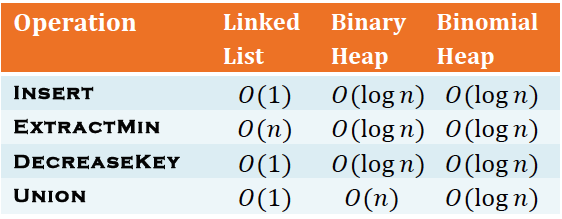
\includegraphics[width=3in]{L7-heaptablebinomialheap.png} 
%	\end{center}
%\end{figure}

\begin{table}[!ht]
\centering
\begin{tabular}{ p{2.4cm}p{1.1cm}p{1.3cm}p{1.4cm} }
\hline
 \textcolor{blue}{\textbf{Operation}} & \textcolor{blue}{\textbf{Linked List}}  & \textcolor{blue}{\textbf{Binary Heap}} & \textcolor{blue}{\textbf{Binomial Heap}}   \\
 \hline
 {\sc Insert} & $O(1)$ & $O(\log n)$ & $O(\log n)$     \\
 {\sc ExtractMin} & $O(n)$ & $O(\log n)$ & $O(\log n)$    \\
 {\sc DecreaseKey} & $O(1)$ & $O(\log n)$ & $O(\log n)$    \\
 {\sc Union} & $O(1)$ & $O(n)$ & $O(\log n)$   \\
 \hline
\end{tabular}
\end{table}

}

\frame{
	\begin{block}{}
		Binomial heap:  more accurate analysis using the amortized technique  
	\end{block}
}

\frame{
	\frametitle{Amortized analysis of {\sc Insert}}



Motivation: 	
\begin{itemize}
	\item If an {\sc Insert} takes a long time (say $\log n$), the subsequent {\sc Insert} operations shouldn't take long! 
	\begin{figure}
     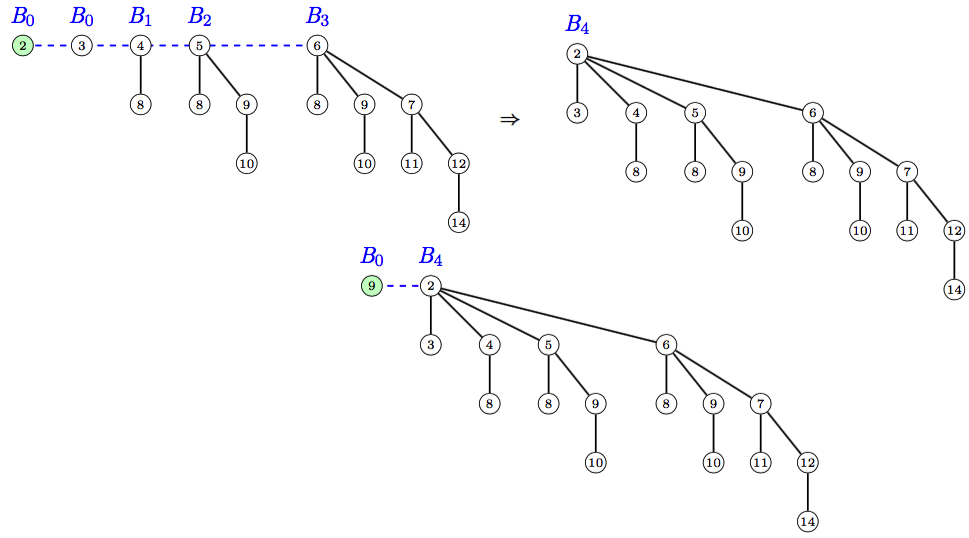
\includegraphics[width=3.9in]{L7-insertexample1.png}
\end{figure}	
	\item Thus, it will be more accurate to examine a sequence of operations rather than each operation individually. 

\end{itemize}
} 	



\frame{
	\frametitle{Amortized analysis of {\sc Insert} operation}

{\sc Insert}$(x)$
\begin{algorithmic}[1]
\begin{small}
\STATE Create a $B_0$ tree for $x$; 
\STATE Change the pointer to the minimum root node if necessary; 
\WHILE{ there are two $B_k$ trees for some $k$}
\STATE Link them together into one $B_{k+1}$ tree; 
\STATE Change the pointer to the minimum root node if necessary; 
\ENDWHILE	
\end{small}
\end{algorithmic}
Analysis:  
\begin{itemize}
	\begin{small}
	\item A single  {\sc Insert} operation takes time $1 + w$, where $w = \#{\tt WHILE}$.
	\item For the sake of calculating the total running time of a sequence  of operations, we 
	represent the running time of a single operation as 
	decrease of a potential function. 

	\item Consider a quantity $\Phi=\#trees$ (called potential function). The changes of $\Phi$ during an operation are: 
	\begin{itemize}
		\item $\Phi$ increase: $1$.
		\item $\Phi$ decrease: $w$. 
	\end{itemize}
%	\item The net $\Phi$ decrease: $w-1$; 
	\item Thus the running time of  {\sc Insert} can be rewritten in terms of $\Phi$ as $1 + w =  1 + $ decrease in $\Phi$. Note that this representation makes  it convenient to sum running time of a sequence of {\sc Insert} operations. 
	\end{small}
\end{itemize}

} 	


\frame{
	\frametitle{Amortized analysis of {\sc ExtractMin} }

{\sc ExtractMin}$()$
\begin{algorithmic}[1]
\begin{small}
%\STATE find min of all roots; 
\STATE Remove the min node, and insert its children to the root list;  
\STATE Change the pointer to the minimum root node if necessary; 
\WHILE{ there are two $B_k$ trees for some $k$}
\STATE Link them together into one $B_{k+1}$ tree; 
\STATE Change the pointer to the minimum root node if necessary; 
\ENDWHILE
\end{small}	
\end{algorithmic}
Analysis: 
\begin{itemize}
\begin{small}
	\item  A single {\sc ExtractMin} operation takes $d  + w$ time, where $d$
denotes degree of the removed root node, and $w = \#${\tt WHILE}.
	\item For the sake of calculating the total running time of a sequence  of operations, we 
	represent the running time of a single operation as 
	decrease of a potential function. 
 
\item Consider a potential function $\Phi = \#trees$. The changes during an operation are: 
	\begin{itemize}
		\item $\Phi$ increase: $d$.
		\item $\Phi$ decrease: $w$.
	\end{itemize}

%\item Net $\Phi$ decrease: $w - d$;
	\item Similarly, the running time is rewritten in terms of $\Phi$ as $d + w =   d + $ decrease in $\#trees$. Note that  $d \leq \log n$. 
\end{small}	
\end{itemize}

}  


\frame{
	\frametitle{Amortized analysis}

\begin{itemize}
	\item Let's consider any sequence of $n$  {\sc Insert} and $m$ {\sc ExtractMin} operations.
	\item The total running time is  at most $n +  m \log n  + $ total decrease in $\#trees$. 
	\item Note: total decrease in $\#trees \leq $ total increase in $\#trees$ (why?), which is at most $n + m  \log n$. 
	\item Thus the total time is at most $2 n + 2 m \log n$. 
	\item We say {\sc Insert} takes $O(1)$ amortized time, and {\sc ExtractMin} takes $O(\log n)$ amortized time.  
\end{itemize}


\begin{definition}[Amortized time]
For any sequence of $n_1$ operation 1, $n_2$ operation $2$..., if the total time is $O(n_1 T_1 + n_2 T_2...)$, we say that operation 1 takes $T_1$ amortized time, operation 2 takes $T_2$ amortized time .... 
\end{definition} 	
}


\frame{
	\frametitle{Intuition of the amortized analysis}

\begin{itemize}
\item 
The actual running time of an {\sc Insert} operation is $1+w$. A large $w$ means that the {\sc Insert} operation takes a long time. Note that the $w$ time was spent on ``decreasing trees"; thus, if the $w$ time was  amortized over the operations ``creating trees",  the ``amortized time" of  {\sc Insert} operation will be only $O(1)$. \ \\
\item The actual running time of an {\sc ExtractMin} operation is at most  $\log n + w$. Note that at most $\log n$ new trees are created during an {\sc ExtractMin} operation; thus, the amortized time is still $O(\log n)$ even if some costs have been amortized to it from other operations due to ``tree creating".  
\end{itemize}

} 



 

\frame{
	\frametitle{Implementing priority queue: Binomial heap} 
%\begin{figure}
%	\begin{center}
%     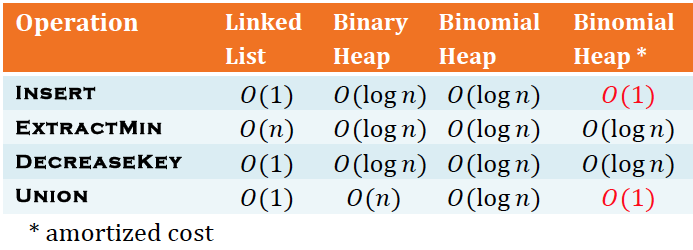
\includegraphics[width=3.4in]{L7-heaptablebinomialheap2.png} 
%	\end{center}
%\end{figure}


\begin{table}[!ht]
\centering
\begin{tabular}{ p{2.4cm}p{1.1cm}p{1.3cm}p{1.4cm}p{1.4cm}}
\hline
 \textcolor{blue}{\textbf{Operation}} & \textcolor{blue}{\textbf{Linked List}}  & \textcolor{blue}{\textbf{Binary Heap}} & \textcolor{blue}{\textbf{Binomial Heap}} & \textcolor{blue}{\textbf{Binomial Heap*}} \\
 \hline
 {\sc Insert} & $O(1)$ & $O(\log n)$ & $O(\log n)$  & \textcolor{red}{$O(1)$}  \\
 {\sc ExtractMin} & $O(n)$ & $O(\log n)$ & $O(\log n)$ & $O(\log n)$  \\
 {\sc DecreaseKey} & $O(1)$ & $O(\log n)$ & $O(\log n)$ & $O(\log n)$  \\
 {\sc Union} & $O(1)$ & $O(n)$ & $O(\log n)$ & \textcolor{red}{$O(1)$}  \\
 \hline
\end{tabular}
\end{table}
*amortized cost


}

\frame{
	\frametitle{ Binomial heap: {\sc DecreaseKey} operation} 

\begin{figure}
\begin{tikzpicture}[scale=1., auto,swap]

  \def\dx{0};
  \def\dy{0}; 
  \def\u{0.8};
  
   \foreach \x/\y/\name/\label in { 0/0/root/0, 0/-1/L11/8, 1/-1/L12/9, 2/-1/L13/7, 4/-1/L14/5} 
          \node[smallvertex,draw=black, fill=white!20] (\name) at (\x*\u+\dx, \y + \dy) {\tiny $\label$};
  
   \foreach \x/\y/\name/\label in {1/-2/L21/10, 2/-2/L22/11/, 3/-2/L23/12, 4/-2/L24/11, 5/-2/L25/12, 6/-2/L26/13}
          \node[smallvertex,draw=black, fill=white!20] (\name) at (\x*\u+\dx, \y + \dy) {\tiny $\label$};

   \foreach \x/\y/\name/\label in {3/-3/L31/14, 5/-3/L32/14, 6/-3/L33/15, 7/-3/L34/16}
          \node[smallvertex,draw=black, fill=white!20] (\name) at (\x*\u+\dx, \y + \dy) {\tiny $\label$};


   \foreach \x/\y/\name/\label in {7/-4/L41/17}
          \node[smallvertex,draw=black, fill=green!20] (\name) at (\x*\u+\dx, \y + \dy) {\tiny $\label$};

  
  \foreach \source/ \dest /\weight in {root/L11/{}, root/L12/{}, root/L13/{}, root/L14/{}}
         \path[undirectededge] (\source) -- node[weight] {$\weight$} (\dest);
 
  \foreach \source/ \dest /\weight in {L12/L21/{}, L13/L22/{}, L13/L23/{}, L14/L24/{}, L14/L25/{}, L14/L26/{}, L23/L31/{}, L25/L32/{}, L26/L33/{}, L26/L34/{}, L34/L41/{}}
         \path[undirectededge] (\source) -- node[weight] {$\weight$} (\dest);
 

  \node[above, blue, ultra thick] at (root.north) {$B_4$};
  


   \end{tikzpicture}
   \caption{{\sc DecreaseKey}:   17 to 1} 
\end{figure}

\begin{itemize}
	\item Time: $O(\log n)$ since in the worst case, we need to perform node exchanging up to the root. 
	\item Question: is there a quicker way for decrease key? 
\end{itemize}
	
}


\frame{
	\begin{block}{}
		Fibonacci heap: an efficient implementation of {\sc DecreaseKey} via simply cutting an edge  rather than exchanging nodes 
	\end{block}
} 

\frame{
	\frametitle{Fibonacci heap} 
		
	\begin{figure}
     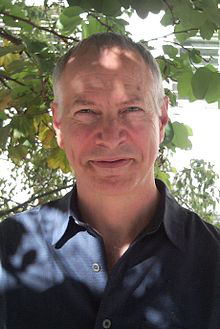
\includegraphics[width=1.5in]{Tarjan.png}
 \caption{Robert Tarjan [1986]} 
\end{figure}
}

\frame{
	\frametitle{Fibonacci heap: an efficient {\sc DecreaseKey} operation} 
	\begin{itemize}
	           \item Basic idea: 
	           	\begin{itemize}
			\item \textcolor{blue}{\bf loosing the structure}: Binomial heap  requires trees to be in perfect shape. Now we loose this restriction --- when heap order is violated, a simple solution is to ``cut off a node, and insert it into the root list". 
			\item \textcolor{blue}{\bf but don't loose it too much}: the ``cutting off" operation makes a  tree not ``binomial" any more; however, it should not deviate from a binomial tree too much. A technique to achieve this objective is allowing any non-root node to lose ``at most one child". 
			\end{itemize}	
\begin{figure}
\begin{minipage}{0.45\textwidth}%
	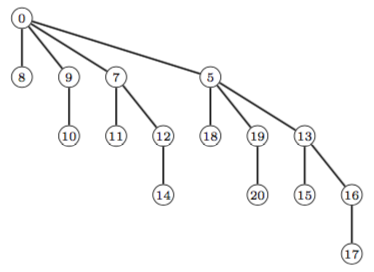
\includegraphics[width=\textwidth]{L7-Fibonacciheaporiginal.png}
\end{minipage}
\begin{minipage}{0.45\textwidth}%
	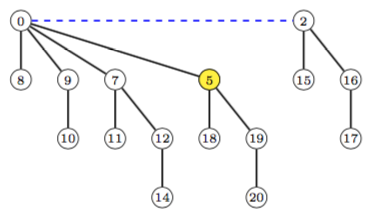
\includegraphics[width=\textwidth]{L7-Fibonacciheapdecreasekey.png}
\end{minipage}
\caption{ Heap order is violated when {\sc DescreaseKey} 13 to 2. However, the heap order can be easily restored via ``cutting off" the node, and inserting it into the root list}
\end{figure}				
	\end{itemize}	


	
}

\frame{
	\frametitle{Fibonacci heap: {\sc DescreaseKey} }

{\sc DecreaseKey}$(v, x)$
\begin{algorithmic}[1]
\STATE $key(v) = x;$
\IF{ heap order is violated}
\STATE $u = v's$ parent; 
\STATE Cut subtree rooted at node $v$, and insert it into the root list;
\STATE Change the pointer to the minimum root node if necessary;  
\WHILE{ $u$ is marked} 
\STATE Cut subtree rooted at node $u$, and insert it into the root list;
\STATE Change the pointer to the minimum root node if necessary;  
\STATE Unmark $u$;  
\STATE $u = u's$ parent; 
\ENDWHILE	
\STATE Mark $u$; 
\ENDIF
\end{algorithmic}
} 


\frame[allowframebreaks]{
\frametitle{ {\sc DecreaseKey}: an example}

\begin{figure}
\begin{tikzpicture}[scale=1., auto,swap]

  \def\dx{0};
  \def\dy{0}; 
  \def\u{0.8};
  
   \foreach \x/\y/\name/\label in { 0/0/root/0, 0/-1/L11/8, 1/-1/L12/9, 2/-1/L13/7, 4/-1/L14/5} 
          \node[smallvertex,draw=black, fill=white!20] (\name) at (\x*\u+\dx, \y + \dy) {\tiny $\label$};
  
   \foreach \x/\y/\name/\label in {1/-2/L21/10, 2/-2/L22/11/, 3/-2/L23/12, 4/-2/L24/18, 5/-2/L25/19, 6/-2/L26/13}
          \node[smallvertex,draw=black, fill=white!20] (\name) at (\x*\u+\dx, \y + \dy) {\tiny $\label$};

   \foreach \x/\y/\name/\label in {3/-3/L31/14, 5/-3/L32/20, 6/-3/L33/15, 7/-3/L34/16}
          \node[smallvertex,draw=black, fill=white!20] (\name) at (\x*\u+\dx, \y + \dy) {\tiny $\label$};


   \foreach \x/\y/\name/\label in {7/-4/L41/17}
          \node[smallvertex,draw=black, fill=white!20] (\name) at (\x*\u+\dx, \y + \dy) {\tiny $\label$};

  
  \foreach \source/ \dest /\weight in {root/L11/{}, root/L12/{}, root/L13/{}, root/L14/{}}
         \path[undirectededge] (\source) -- node[weight] {$\weight$} (\dest);
 
  \foreach \source/ \dest /\weight in {L12/L21/{}, L13/L22/{}, L13/L23/{}, L14/L24/{}, L14/L25/{}, L14/L26/{}, L23/L31/{}, L25/L32/{}, L26/L33/{}, L26/L34/{}, L34/L41/{}}
         \path[undirectededge] (\source) -- node[weight] {$\weight$} (\dest);
 

  
   \end{tikzpicture}
   \caption[1]{A  Fibonacci heap. To  {\sc DecreaseKey}: 19 to 3. }
\end{figure}


\begin{figure}
\begin{tikzpicture}[scale=1., auto,swap]

  \def\dx{0};
  \def\dy{0}; 
  \def\u{0.8};
  
   \foreach \x/\y/\name/\label in { 0/0/root/0, 0/-1/L11/8, 1/-1/L12/9, 2/-1/L13/7, 4/-1/L14/5} 
          \node[smallvertex,draw=black, fill=white!20] (\name) at (\x*\u+\dx, \y + \dy) {\tiny $\label$};
  
   \foreach \x/\y/\name/\label in {1/-2/L21/10, 2/-2/L22/11/, 3/-2/L23/12, 4/-2/L24/18, 5/0/L3/3, 6/-2/L26/13}
          \node[smallvertex,draw=black, fill=white!20] (\name) at (\x*\u+\dx, \y + \dy) {\tiny $\label$};

   \foreach \x/\y/\name/\label in {3/-3/L31/14, 5/-1/L20/20, 6/-3/L33/15, 7/-3/L34/16}
          \node[smallvertex,draw=black, fill=white!20] (\name) at (\x*\u+\dx, \y + \dy) {\tiny $\label$};


   \foreach \x/\y/\name/\label in {7/-4/L41/17}
          \node[smallvertex,draw=black, fill=white!20] (\name) at (\x*\u+\dx, \y + \dy) {\tiny $\label$};

  
  \foreach \source/ \dest /\weight in {root/L11/{}, root/L12/{}, root/L13/{}, root/L14/{}}
         \path[undirectededge] (\source) -- node[weight] {$\weight$} (\dest);
 
  \foreach \source/ \dest /\weight in {L12/L21/{}, L13/L22/{}, L13/L23/{}, L14/L24/{}, L14/L26/{}, L23/L31/{}, L3/L20/{}, L26/L33/{}, L26/L34/{}, L34/L41/{}}
         \path[undirectededge] (\source) -- node[weight] {$\weight$} (\dest);
 


%marks
  \foreach \x/\y/\name/\label in { 4/-1/L14/5} 
          \node[smallvertex,draw=black, fill=yellow] (\name) at (\x*\u+\dx, \y + \dy) {\tiny $\label$};


  \foreach \source/ \dest /\weight in {root/L3/{}}
           \path[undirectededge, dashed, blue, thick] (\source) -- node[weight] {$\weight$} (\dest);

  
   \end{tikzpicture}
   \caption{After {\sc DecreaseKey}: 19 to 3. To {\sc DecreaseKey}: 15 to 2.  }
\end{figure}



\begin{figure}
\begin{tikzpicture}[scale=1., auto,swap]

  \def\dx{0};
  \def\dy{0}; 
  \def\u{0.8};
  
   \foreach \x/\y/\name/\label in { 0/0/root/0, 0/-1/L11/8, 1/-1/L12/9, 2/-1/L13/7, 4/-1/L14/5} 
          \node[smallvertex,draw=black, fill=white!20] (\name) at (\x*\u+\dx, \y + \dy) {\tiny $\label$};
  
   \foreach \x/\y/\name/\label in {1/-2/L21/10, 2/-2/L22/11/, 3/-2/L23/12, 4/-2/L24/18, 5/0/L3/3, 6/-2/L26/13}
          \node[smallvertex,draw=black, fill=white!20] (\name) at (\x*\u+\dx, \y + \dy) {\tiny $\label$};

   \foreach \x/\y/\name/\label in {3/-3/L31/14, 5/-1/L20/20, 6/0/L2/2, 7/-3/L34/16}
          \node[smallvertex,draw=black, fill=white!20] (\name) at (\x*\u+\dx, \y + \dy) {\tiny $\label$};


   \foreach \x/\y/\name/\label in {7/-4/L41/17}
          \node[smallvertex,draw=black, fill=white!20] (\name) at (\x*\u+\dx, \y + \dy) {\tiny $\label$};

  
  \foreach \source/ \dest /\weight in {root/L11/{}, root/L12/{}, root/L13/{}, root/L14/{}}
         \path[undirectededge] (\source) -- node[weight] {$\weight$} (\dest);
 
  \foreach \source/ \dest /\weight in {L12/L21/{}, L13/L22/{}, L13/L23/{}, L14/L24/{}, L14/L26/{}, L23/L31/{}, L3/L20/{}, L26/L34/{}, L34/L41/{}}
         \path[undirectededge] (\source) -- node[weight] {$\weight$} (\dest);
 


%marks
  \foreach \x/\y/\name/\label in { 4/-1/L14/5, 6/-2/L13/13 } 
          \node[smallvertex,draw=black, fill=yellow] (\name) at (\x*\u+\dx, \y + \dy) {\tiny $\label$};


  \foreach \source/ \dest /\weight in {root/L3/{}, L3/L2/{}}
           \path[undirectededge, dashed, blue, thick] (\source) -- node[weight] {$\weight$} (\dest);

  
   \end{tikzpicture}
     \caption{After {\sc DecreaseKey}: 15 to 2. To {\sc DecreaseKey}: 12 to 8. }

\end{figure}



\begin{figure}
\begin{tikzpicture}[scale=1., auto,swap]

  \def\dx{0};
  \def\dy{0}; 
  \def\u{0.8};
  
   \foreach \x/\y/\name/\label in { 0/0/root/0, 0/-1/L11/8, 1/-1/L12/9, 2/-1/L13/7, 4/-1/L14/5} 
          \node[smallvertex,draw=black, fill=white!20] (\name) at (\x*\u+\dx, \y + \dy) {\tiny $\label$};
  
   \foreach \x/\y/\name/\label in {1/-2/L21/10, 2/-2/L22/11/, 3/-2/L23/8, 4/-2/L24/18, 5/0/L3/3, 6/-2/L26/13}
          \node[smallvertex,draw=black, fill=white!20] (\name) at (\x*\u+\dx, \y + \dy) {\tiny $\label$};

   \foreach \x/\y/\name/\label in {3/-3/L31/14, 5/-1/L20/20, 6/0/L2/2, 7/-3/L34/16}
          \node[smallvertex,draw=black, fill=white!20] (\name) at (\x*\u+\dx, \y + \dy) {\tiny $\label$};


   \foreach \x/\y/\name/\label in {7/-4/L41/17}
          \node[smallvertex,draw=black, fill=white!20] (\name) at (\x*\u+\dx, \y + \dy) {\tiny $\label$};

  
  \foreach \source/ \dest /\weight in {root/L11/{}, root/L12/{}, root/L13/{}, root/L14/{}}
         \path[undirectededge] (\source) -- node[weight] {$\weight$} (\dest);
 
  \foreach \source/ \dest /\weight in {L12/L21/{}, L13/L22/{}, L13/L23/{}, L14/L24/{}, L14/L26/{}, L23/L31/{}, L3/L20/{}, L26/L34/{}, L34/L41/{}}
         \path[undirectededge] (\source) -- node[weight] {$\weight$} (\dest);
 


%marks
  \foreach \x/\y/\name/\label in { 4/-1/L14/5, 6/-2/L13/13 } 
          \node[smallvertex,draw=black, fill=yellow] (\name) at (\x*\u+\dx, \y + \dy) {\tiny $\label$};


  \foreach \source/ \dest /\weight in {root/L3/{}, L3/L2/{}}
           \path[undirectededge, dashed, blue, thick] (\source) -- node[weight] {$\weight$} (\dest);

  
   \end{tikzpicture}
     \caption{After {\sc DecreaseKey}: 12 to 8. To {\sc DecreaseKey}: 14 to 1. }

\end{figure}


\begin{figure}
\begin{tikzpicture}[scale=1., auto,swap]

  \def\dx{0};
  \def\dy{0}; 
  \def\u{0.8};
  
   \foreach \x/\y/\name/\label in { 0/0/root/0, 0/-1/L11/8, 1/-1/L12/9, 2/-1/L13/7, 4/-1/L14/5} 
          \node[smallvertex,draw=black, fill=white!20] (\name) at (\x*\u+\dx, \y + \dy) {\tiny $\label$};
  
   \foreach \x/\y/\name/\label in {1/-2/L21/10, 2/-2/L22/11/, 3/-2/L23/8, 4/-2/L24/18, 5/0/L3/3, 6/-2/L26/13}
          \node[smallvertex,draw=black, fill=white!20] (\name) at (\x*\u+\dx, \y + \dy) {\tiny $\label$};

   \foreach \x/\y/\name/\label in {-1/0/L1/1, 5/-1/L20/20, 6/0/L2/2, 7/-3/L34/16}
          \node[smallvertex,draw=black, fill=white!20] (\name) at (\x*\u+\dx, \y + \dy) {\tiny $\label$};


   \foreach \x/\y/\name/\label in {7/-4/L41/17}
          \node[smallvertex,draw=black, fill=white!20] (\name) at (\x*\u+\dx, \y + \dy) {\tiny $\label$};

  
  \foreach \source/ \dest /\weight in {root/L11/{}, root/L12/{}, root/L13/{}, root/L14/{}}
         \path[undirectededge] (\source) -- node[weight] {$\weight$} (\dest);
 
  \foreach \source/ \dest /\weight in {L12/L21/{}, L13/L22/{}, L13/L23/{}, L14/L24/{}, L14/L26/{}, L3/L20/{}, L26/L34/{}, L34/L41/{}}
         \path[undirectededge] (\source) -- node[weight] {$\weight$} (\dest);
 


%marks
  \foreach \x/\y/\name/\label in { 3/-2/L23/8, 4/-1/L14/5, 6/-2/L13/13 } 
          \node[smallvertex,draw=black, fill=yellow] (\name) at (\x*\u+\dx, \y + \dy) {\tiny $\label$};


  \foreach \source/ \dest /\weight in {L1/root/{}, root/L3/{}, L3/L2/{}}
           \path[undirectededge, dashed, blue, thick] (\source) -- node[weight] {$\weight$} (\dest);

  
   \end{tikzpicture}
     \caption{After {\sc DecreaseKey}: 14 to 1. To {\sc DecreaseKey}: 16 to 9. }

\end{figure}



\begin{figure}
\begin{tikzpicture}[scale=1., auto,swap]

  \def\dx{0};
  \def\dy{0}; 
  \def\u{0.8};
  
   \foreach \x/\y/\name/\label in { 0/0/root/0, 0/-1/L11/8, 1/-1/L12/9, 2/-1/L7/7, 4/0/L5/5} 
          \node[smallvertex,draw=black, fill=white!20] (\name) at (\x*\u+\dx, \y + \dy) {\tiny $\label$};
  
   \foreach \x/\y/\name/\label in {1/-2/L21/10, 2/-2/L22/11/, 3/-2/L23/8, 4/-1/L24/18, 5/0/L3/3, 7/0/L13/13}
          \node[smallvertex,draw=black, fill=white!20] (\name) at (\x*\u+\dx, \y + \dy) {\tiny $\label$};

   \foreach \x/\y/\name/\label in {-1/0/L1/1, 5/-1/L20/20, 6/0/L2/2, 8/0/L9/9}
          \node[smallvertex,draw=black, fill=white!20] (\name) at (\x*\u+\dx, \y + \dy) {\tiny $\label$};


   \foreach \x/\y/\name/\label in {8/-1/L41/17}
          \node[smallvertex,draw=black, fill=white!20] (\name) at (\x*\u+\dx, \y + \dy) {\tiny $\label$};

  
  \foreach \source/ \dest /\weight in {root/L11/{}, root/L12/{}, root/L7/{}}
         \path[undirectededge] (\source) -- node[weight] {$\weight$} (\dest);
 
  \foreach \source/ \dest /\weight in {L12/L21/{}, L7/L22/{}, L7/L23/{}, L14/L24/{},  L3/L20/{}, L9/L41/{}, L5/L24/{}}
         \path[undirectededge] (\source) -- node[weight] {$\weight$} (\dest);
 


%marks
   \foreach \x/\y/\name/\label in {3/-2/L23/8}
          \node[smallvertex,draw=black, fill=yellow] (\name) at (\x*\u+\dx, \y + \dy) {\tiny $\label$};



  \foreach \source/ \dest /\weight in {L1/root/{}, root/L5/{}, L5/L3/{},  L3/L2/{}, L2/L13/{}, L13/L9/{}}
           \path[undirectededge, dashed, blue, thick] (\source) -- node[weight] {$\weight$} (\dest);

  
   \end{tikzpicture}
     \caption{After {\sc DecreaseKey}: 16 to 9 }

\end{figure}

}



\frame{
	\frametitle{Fibonacci heap: {\sc Insert} }

{\sc Insert}$(x)$
\begin{algorithmic}[1]
\STATE Create a tree for $x$, and insert it into the root list; 
\STATE Change the pointer to the minimum root node if necessary;  
\end{algorithmic}
Note: \textcolor{red}{\bf Being lazy!} Consolidating trees when extracting minimum.  \\
\begin{figure}
\begin{tikzpicture}[scale=1., auto,swap]

  \def\dx{0};
  \def\dy{0}; 
  \def\u{0.8};
  
   \foreach \x/\y/\name/\label in { 0/0/root/0, 0/-1/L11/8, 1/-1/L12/9, 2/-1/L7/7, 4/0/L5/5} 
          \node[smallvertex,draw=black, fill=white!20] (\name) at (\x*\u+\dx, \y + \dy) {\tiny $\label$};
  
   \foreach \x/\y/\name/\label in {1/-2/L21/10, 2/-2/L22/11/, 3/-2/L23/8, 4/-1/L24/18, 5/0/L3/3, 7/0/L13/13}
          \node[smallvertex,draw=black, fill=white!20] (\name) at (\x*\u+\dx, \y + \dy) {\tiny $\label$};

   \foreach \x/\y/\name/\label in {-1/0/L1/1, 5/-1/L20/20, 6/0/L2/2, 8/0/L9/9}
          \node[smallvertex,draw=black, fill=white!20] (\name) at (\x*\u+\dx, \y + \dy) {\tiny $\label$};


   \foreach \x/\y/\name/\label in {8/-1/L41/17}
          \node[smallvertex,draw=black, fill=white!20] (\name) at (\x*\u+\dx, \y + \dy) {\tiny $\label$};

  
  \foreach \source/ \dest /\weight in {root/L11/{}, root/L12/{}, root/L7/{}}
         \path[undirectededge] (\source) -- node[weight] {$\weight$} (\dest);
 
  \foreach \source/ \dest /\weight in {L12/L21/{}, L7/L22/{}, L7/L23/{}, L14/L24/{},  L3/L20/{}, L9/L41/{}, L5/L24/{}}
         \path[undirectededge] (\source) -- node[weight] {$\weight$} (\dest);
 


%marks
   \foreach \x/\y/\name/\label in {3/-2/L23/8}
          \node[smallvertex,draw=black, fill=yellow] (\name) at (\x*\u+\dx, \y + \dy) {\tiny $\label$};



  \foreach \source/ \dest /\weight in {L1/root/{}, root/L5/{}, L5/L3/{},  L3/L2/{}, L2/L13/{}, L13/L9/{}}
           \path[undirectededge, dashed, blue, thick] (\source) -- node[weight] {$\weight$} (\dest);

  
   \end{tikzpicture}
\end{figure}
\begin{figure}
\begin{tikzpicture}[scale=1., auto,swap]

  \def\dx{0};
  \def\dy{0}; 
  \def\u{0.8};
  
   \foreach \x/\y/\name/\label in { 0/0/root/0, 0/-1/L11/8, 1/-1/L12/9, 2/-1/L7/7, 4/0/L5/5} 
          \node[smallvertex,draw=black, fill=white!20] (\name) at (\x*\u+\dx, \y + \dy) {\tiny $\label$};
  
   \foreach \x/\y/\name/\label in {1/-2/L21/10, 2/-2/L22/11/, 3/-2/L23/8, 4/-1/L24/18, 5/0/L3/3, 7/0/L13/13}
          \node[smallvertex,draw=black, fill=white!20] (\name) at (\x*\u+\dx, \y + \dy) {\tiny $\label$};

   \foreach \x/\y/\name/\label in {-1/0/L1/1, 5/-1/L20/20, 6/0/L2/2, 8/0/L9/9, 9/0/L6/6}
          \node[smallvertex,draw=black, fill=white!20] (\name) at (\x*\u+\dx, \y + \dy) {\tiny $\label$};


   \foreach \x/\y/\name/\label in {8/-1/L41/17}
          \node[smallvertex,draw=black, fill=white!20] (\name) at (\x*\u+\dx, \y + \dy) {\tiny $\label$};

  
  \foreach \source/ \dest /\weight in {root/L11/{}, root/L12/{}, root/L7/{}}
         \path[undirectededge] (\source) -- node[weight] {$\weight$} (\dest);
 
  \foreach \source/ \dest /\weight in {L12/L21/{}, L7/L22/{}, L7/L23/{}, L14/L24/{},  L3/L20/{}, L9/L41/{}, L5/L24/{}}
         \path[undirectededge] (\source) -- node[weight] {$\weight$} (\dest);
 


%marks
   \foreach \x/\y/\name/\label in {3/-2/L23/8}
          \node[smallvertex,draw=black, fill=yellow] (\name) at (\x*\u+\dx, \y + \dy) {\tiny $\label$};



  \foreach \source/ \dest /\weight in {L1/root/{}, root/L5/{}, L5/L3/{},  L3/L2/{}, L2/L13/{}, L13/L9/{}, L9/L6/{}}
           \path[undirectededge, dashed, blue, thick] (\source) -- node[weight] {$\weight$} (\dest);

  
   \end{tikzpicture}
   \caption{{\sc Insert(6)}: creating a new tree, and insert it into the root list}
\end{figure}

}

\frame{
	\frametitle{Fibonacci heap: {\sc ExtractMin} }

{\sc ExtractMin}$()$
\begin{algorithmic}[1]
\STATE Remove the min node, and insert its children into the root list; 
\STATE Change the pointer to the minimum root node if necessary;  
\WHILE{ there are two roots $u$ and $v$ of the same degree} 
\STATE Consolidate the two trees together;
\STATE Change the pointer to the minimum root node if necessary;  
\ENDWHILE	
\end{algorithmic}
} 


\frame[allowframebreaks]{
\frametitle{ {\sc ExtractMin}: an example }


\begin{figure}
\begin{tikzpicture}[scale=1., auto,swap]

  \def\dx{0};
  \def\dy{0}; 
  \def\u{0.8};
  
   \foreach \x/\y/\name/\label in { 0/0/root/0, 0/-1/L11/8, 1/-1/L12/9, 2/-1/L7/7, 4/0/L5/5} 
          \node[smallvertex,draw=black, fill=white!20] (\name) at (\x*\u+\dx, \y + \dy) {\tiny $\label$};
  
   \foreach \x/\y/\name/\label in {1/-2/L21/10, 2/-2/L22/11/, 3/-2/L23/8, 4/-1/L24/18, 5/0/L3/3, 7/0/L13/13}
          \node[smallvertex,draw=black, fill=white!20] (\name) at (\x*\u+\dx, \y + \dy) {\tiny $\label$};

   \foreach \x/\y/\name/\label in {-1/0/L1/1, 5/-1/L20/20, 6/0/L2/2, 8/0/L9/9}
          \node[smallvertex,draw=black, fill=white!20] (\name) at (\x*\u+\dx, \y + \dy) {\tiny $\label$};


   \foreach \x/\y/\name/\label in {8/-1/L41/17}
          \node[smallvertex,draw=black, fill=white!20] (\name) at (\x*\u+\dx, \y + \dy) {\tiny $\label$};

  
  \foreach \source/ \dest /\weight in {root/L11/{}, root/L12/{}, root/L7/{}}
         \path[undirectededge, red] (\source) -- node[weight] {$\weight$} (\dest);
 
  \foreach \source/ \dest /\weight in {L12/L21/{}, L7/L22/{}, L7/L23/{}, L14/L24/{},  L3/L20/{}, L9/L41/{}, L5/L24/{}}
         \path[undirectededge] (\source) -- node[weight] {$\weight$} (\dest);
 


%marks
   \foreach \x/\y/\name/\label in {0/0/root/0}
          \node[smallvertex,draw=black, fill=green] (\name) at (\x*\u+\dx, \y + \dy) {\tiny $\label$};

   \foreach \x/\y/\name/\label in {3/-2/L23/8}
          \node[smallvertex,draw=black, fill=yellow] (\name) at (\x*\u+\dx, \y + \dy) {\tiny $\label$};



  \foreach \source/ \dest /\weight in {L1/root/{}, root/L5/{}, L5/L3/{},  L3/L2/{}, L2/L13/{}, L13/L9/{}}
           \path[undirectededge, dashed, blue, thick] (\source) -- node[weight] {$\weight$} (\dest);

  
   \end{tikzpicture}
\end{figure}

\begin{figure}
\begin{tikzpicture}[scale=1., auto,swap]

  \def\dx{0};
  \def\dy{0}; 
  \def\u{0.8};
  
   \foreach \x/\y/\name/\label in { 0/0/root/, 0/0/L11/8, 1/0/L12/9, 2/0/L7/7, 4/0/L5/5} 
          \node[smallvertex,draw=black, fill=white!20] (\name) at (\x*\u+\dx, \y + \dy) {\tiny $\label$};
  
   \foreach \x/\y/\name/\label in {1/-1/L21/10, 2/-1/L22/11/, 3/-1/L23/8, 4/-1/L24/18, 5/0/L3/3, 7/0/L13/13}
          \node[smallvertex,draw=black, fill=white!20] (\name) at (\x*\u+\dx, \y + \dy) {\tiny $\label$};

   \foreach \x/\y/\name/\label in {-1/0/L1/1, 5/-1/L20/20, 6/0/L2/2, 8/0/L9/9}
          \node[smallvertex,draw=black, fill=white!20] (\name) at (\x*\u+\dx, \y + \dy) {\tiny $\label$};


   \foreach \x/\y/\name/\label in {8/-1/L41/17}
          \node[smallvertex,draw=black, fill=white!20] (\name) at (\x*\u+\dx, \y + \dy) {\tiny $\label$};

   
  \foreach \source/ \dest /\weight in {L12/L21/{}, L7/L22/{}, L7/L23/{}, L14/L24/{},  L3/L20/{}, L9/L41/{}, L5/L24/{}}
         \path[undirectededge] (\source) -- node[weight] {$\weight$} (\dest);
 


%marks

   \foreach \x/\y/\name/\label in {3/-1/L23/8}
          \node[smallvertex,draw=black, fill=yellow] (\name) at (\x*\u+\dx, \y + \dy) {\tiny $\label$};



  \foreach \source/ \dest /\weight in {L1/root/{}, root/L12/{}, L12/L7/{},L7/L5/{},L5/L3/{},  L3/L2/{}, L2/L13/{}, L13/L9/{}}
           \path[undirectededge, dashed, blue, thick] (\source) -- node[weight] {$\weight$} (\dest);

  
   \end{tikzpicture}
     \caption{{\sc ExtractMin}: removing the min node, and adding 3 trees }
\end{figure}





\begin{figure}
\begin{tikzpicture}[scale=1., auto,swap]

  \def\dx{0};
  \def\dy{0}; 
  \def\u{0.8};
  
   \foreach \x/\y/\name/\label in {  0/-1/L8/8, 1/0/L12/9, 2/0/L7/7, 4/0/L5/5} 
          \node[smallvertex,draw=black, fill=white!20] (\name) at (\x*\u+\dx, \y + \dy) {\tiny $\label$};
  
   \foreach \x/\y/\name/\label in {1/-1/L21/10, 2/-1/L22/11/, 3/-1/L23/8, 4/-1/L24/18, 5/0/L3/3, 7/0/L13/13}
          \node[smallvertex,draw=black, fill=white!20] (\name) at (\x*\u+\dx, \y + \dy) {\tiny $\label$};

   \foreach \x/\y/\name/\label in {0/0/L1/1, 5/-1/L20/20, 6/0/L2/2, 8/0/L9/9}
          \node[smallvertex,draw=black, fill=white!20] (\name) at (\x*\u+\dx, \y + \dy) {\tiny $\label$};


   \foreach \x/\y/\name/\label in {8/-1/L41/17}
          \node[smallvertex,draw=black, fill=white!20] (\name) at (\x*\u+\dx, \y + \dy) {\tiny $\label$};

   
  \foreach \source/ \dest /\weight in {L1/L8/{}, L12/L21/{}, L7/L22/{}, L7/L23/{}, L14/L24/{},  L3/L20/{}, L9/L41/{}, L5/L24/{}}
         \path[undirectededge] (\source) -- node[weight] {$\weight$} (\dest);
 


%marks

   \foreach \x/\y/\name/\label in {3/-1/L23/8}
          \node[smallvertex,draw=black, fill=yellow] (\name) at (\x*\u+\dx, \y + \dy) {\tiny $\label$};



  \foreach \source/ \dest /\weight in { L1/L12/{}, L12/L7/{},L7/L5/{},L5/L3/{},  L3/L2/{}, L2/L13/{}, L13/L9/{}}
           \path[undirectededge, dashed, blue, thick] (\source) -- node[weight] {$\weight$} (\dest);

  
   \end{tikzpicture}
  \caption{{\sc ExtractMin}: after consolidating two trees rooted at node 1 and 8} 
\end{figure}



\begin{figure}
\begin{tikzpicture}[scale=1., auto,swap]

  \def\dx{0};
  \def\dy{0}; 
  \def\u{0.8};
  
   \foreach \x/\y/\name/\label in {  0/-1/L8/8, 1/-1/L12/9, 2/0/L7/7, 4/0/L5/5} 
          \node[smallvertex,draw=black, fill=white!20] (\name) at (\x*\u+\dx, \y + \dy) {\tiny $\label$};
  
   \foreach \x/\y/\name/\label in {1/-2/L21/10, 2/-1/L22/11/, 3/-1/L23/8, 4/-1/L24/18, 5/0/L3/3, 7/0/L13/13}
          \node[smallvertex,draw=black, fill=white!20] (\name) at (\x*\u+\dx, \y + \dy) {\tiny $\label$};

   \foreach \x/\y/\name/\label in {0/0/L1/1, 5/-1/L20/20, 6/0/L2/2, 8/0/L9/9}
          \node[smallvertex,draw=black, fill=white!20] (\name) at (\x*\u+\dx, \y + \dy) {\tiny $\label$};


   \foreach \x/\y/\name/\label in {8/-1/L41/17}
          \node[smallvertex,draw=black, fill=white!20] (\name) at (\x*\u+\dx, \y + \dy) {\tiny $\label$};

   
  \foreach \source/ \dest /\weight in {L1/L12/{}, L1/L8/{}, L12/L21/{}, L7/L22/{}, L7/L23/{}, L14/L24/{},  L3/L20/{}, L9/L41/{}, L5/L24/{}}
         \path[undirectededge] (\source) -- node[weight] {$\weight$} (\dest);
 


%marks

   \foreach \x/\y/\name/\label in {3/-1/L23/8}
          \node[smallvertex,draw=black, fill=yellow] (\name) at (\x*\u+\dx, \y + \dy) {\tiny $\label$};



  \foreach \source/ \dest /\weight in { L1/L7/{},L7/L5/{},L5/L3/{},  L3/L2/{}, L2/L13/{}, L13/L9/{}}
           \path[undirectededge, dashed, blue, thick] (\source) -- node[weight] {$\weight$} (\dest);

  
   \end{tikzpicture}
     \caption{{\sc ExtractMin}: after consolidating two trees rooted at node 1 and 9} 

\end{figure}



\begin{figure}
\begin{tikzpicture}[scale=1., auto,swap]

  \def\dx{0};
  \def\dy{0}; 
  \def\u{0.8};
  
   \foreach \x/\y/\name/\label in {  0/-1/L8/8, 1/-1/L12/9, 2/-1/L7/7, 4/0/L5/5} 
          \node[smallvertex,draw=black, fill=white!20] (\name) at (\x*\u+\dx, \y + \dy) {\tiny $\label$};
  
   \foreach \x/\y/\name/\label in {1/-2/L21/10, 2/-2/L22/11/, 3/-2/L23/8, 4/-1/L24/18, 5/0/L3/3, 7/0/L13/13}
          \node[smallvertex,draw=black, fill=white!20] (\name) at (\x*\u+\dx, \y + \dy) {\tiny $\label$};

   \foreach \x/\y/\name/\label in {0/0/L1/1, 5/-1/L20/20, 6/0/L2/2, 8/0/L9/9}
          \node[smallvertex,draw=black, fill=white!20] (\name) at (\x*\u+\dx, \y + \dy) {\tiny $\label$};


   \foreach \x/\y/\name/\label in {8/-1/L41/17}
          \node[smallvertex,draw=black, fill=white!20] (\name) at (\x*\u+\dx, \y + \dy) {\tiny $\label$};

   
  \foreach \source/ \dest /\weight in {L1/L8/{}, L1/L7/{}, L1/L12/{}, L12/L21/{}, L7/L22/{}, L7/L23/{}, L14/L24/{},  L3/L20/{}, L9/L41/{}, L5/L24/{}}
         \path[undirectededge] (\source) -- node[weight] {$\weight$} (\dest);
 


%marks

   \foreach \x/\y/\name/\label in {3/-2/L23/8}
          \node[smallvertex,draw=black, fill=yellow] (\name) at (\x*\u+\dx, \y + \dy) {\tiny $\label$};



  \foreach \source/ \dest /\weight in { L1/L5/{},L5/L3/{},  L3/L2/{}, L2/L13/{}, L13/L9/{}}
           \path[undirectededge, dashed, blue, thick] (\source) -- node[weight] {$\weight$} (\dest);

  
   \end{tikzpicture}
  \caption{{\sc ExtractMin}: after consolidating two trees rooted at node 1 and 7} 

\end{figure}



\begin{figure}
\begin{tikzpicture}[scale=1., auto,swap]

  \def\dx{0};
  \def\dy{0}; 
  \def\u{0.8};
  
   \foreach \x/\y/\name/\label in {  0/-1/L8/8, 1/-1/L12/9, 2/-1/L7/7, 4/0/L5/3} 
          \node[smallvertex,draw=black, fill=white!20] (\name) at (\x*\u+\dx, \y + \dy) {\tiny $\label$};
  
   \foreach \x/\y/\name/\label in {1/-2/L21/10, 2/-2/L22/11/, 3/-2/L23/8, 4/-1/L24/20, 5/-1/L3/5, 7/0/L13/13}
          \node[smallvertex,draw=black, fill=white!20] (\name) at (\x*\u+\dx, \y + \dy) {\tiny $\label$};

   \foreach \x/\y/\name/\label in {0/0/L1/1, 5/-2/L20/18, 6/0/L2/2, 8/0/L9/9}
          \node[smallvertex,draw=black, fill=white!20] (\name) at (\x*\u+\dx, \y + \dy) {\tiny $\label$};


   \foreach \x/\y/\name/\label in {8/-1/L41/17}
          \node[smallvertex,draw=black, fill=white!20] (\name) at (\x*\u+\dx, \y + \dy) {\tiny $\label$};

   
  \foreach \source/ \dest /\weight in {L5/L3/{}, L1/L8/{}, L1/L7/{}, L1/L12/{}, L12/L21/{}, L7/L22/{}, L7/L23/{}, L14/L24/{},  L3/L20/{}, L9/L41/{}, L5/L24/{}}
         \path[undirectededge] (\source) -- node[weight] {$\weight$} (\dest);
 


%marks

   \foreach \x/\y/\name/\label in {3/-2/L23/8}
          \node[smallvertex,draw=black, fill=yellow] (\name) at (\x*\u+\dx, \y + \dy) {\tiny $\label$};



  \foreach \source/ \dest /\weight in { L1/L5/{},L5/L2/{}, L2/L13/{}, L13/L9/{}}
           \path[undirectededge, dashed, blue, thick] (\source) -- node[weight] {$\weight$} (\dest);

  
   \end{tikzpicture}
     \caption{{\sc ExtractMin}: after consolidating two trees rooted at node 3 and 5} 

\end{figure}



\begin{figure}
\begin{tikzpicture}[scale=1., auto,swap]

  \def\dx{0};
  \def\dy{0}; 
  \def\u{0.8};
  
   \foreach \x/\y/\name/\label in {  0/-1/L8/8, 1/-1/L12/9, 2/-1/L7/7, 4/0/L5/3} 
          \node[smallvertex,draw=black, fill=white!20] (\name) at (\x*\u+\dx, \y + \dy) {\tiny $\label$};
  
   \foreach \x/\y/\name/\label in {1/-2/L21/10, 2/-2/L22/11/, 3/-2/L23/8, 4/-1/L24/20, 5/-1/L3/5, 6/-1/L13/13}
          \node[smallvertex,draw=black, fill=white!20] (\name) at (\x*\u+\dx, \y + \dy) {\tiny $\label$};

   \foreach \x/\y/\name/\label in {0/0/L1/1, 5/-2/L20/18, 6/0/L2/2, 7/0/L9/9}
          \node[smallvertex,draw=black, fill=white!20] (\name) at (\x*\u+\dx, \y + \dy) {\tiny $\label$};


   \foreach \x/\y/\name/\label in {7/-1/L41/17}
          \node[smallvertex,draw=black, fill=white!20] (\name) at (\x*\u+\dx, \y + \dy) {\tiny $\label$};

   
  \foreach \source/ \dest /\weight in {L2/L13/{}, L5/L3/{}, L1/L8/{}, L1/L7/{}, L1/L12/{}, L12/L21/{}, L7/L22/{}, L7/L23/{}, L14/L24/{},  L3/L20/{}, L9/L41/{}, L5/L24/{}}
         \path[undirectededge] (\source) -- node[weight] {$\weight$} (\dest);
 


%marks

   \foreach \x/\y/\name/\label in {3/-2/L23/8}
          \node[smallvertex,draw=black, fill=yellow] (\name) at (\x*\u+\dx, \y + \dy) {\tiny $\label$};



  \foreach \source/ \dest /\weight in { L1/L5/{},L5/L2/{}, L2/L9/{}}
           \path[undirectededge, dashed, blue, thick] (\source) -- node[weight] {$\weight$} (\dest);

  
   \end{tikzpicture}
     \caption{{\sc ExtractMin}: after consolidating two trees rooted at node 2 and 13} 

\end{figure}



\begin{figure}
\begin{tikzpicture}[scale=1., auto,swap]

  \def\dx{0};
  \def\dy{0}; 
  \def\u{0.8};
  
   \foreach \x/\y/\name/\label in {  0/-1/L8/8, 1/-1/L12/9, 2/-1/L7/7, 4/0/L5/3} 
          \node[smallvertex,draw=black, fill=white!20] (\name) at (\x*\u+\dx, \y + \dy) {\tiny $\label$};
  
   \foreach \x/\y/\name/\label in {1/-2/L21/10, 2/-2/L22/11/, 3/-2/L23/8, 4/-1/L24/20, 5/-1/L3/5, 6/-1/L13/13}
          \node[smallvertex,draw=black, fill=white!20] (\name) at (\x*\u+\dx, \y + \dy) {\tiny $\label$};

   \foreach \x/\y/\name/\label in {0/0/L1/1, 5/-2/L20/18, 6/0/L2/2, 7/-1/L9/9}
          \node[smallvertex,draw=black, fill=white!20] (\name) at (\x*\u+\dx, \y + \dy) {\tiny $\label$};


   \foreach \x/\y/\name/\label in {7/-2/L41/17}
          \node[smallvertex,draw=black, fill=white!20] (\name) at (\x*\u+\dx, \y + \dy) {\tiny $\label$};

   
  \foreach \source/ \dest /\weight in {L2/L9/{},L2/L13/{}, L5/L3/{}, L1/L8/{}, L1/L7/{}, L1/L12/{}, L12/L21/{}, L7/L22/{}, L7/L23/{}, L14/L24/{},  L3/L20/{}, L9/L41/{}, L5/L24/{}}
         \path[undirectededge] (\source) -- node[weight] {$\weight$} (\dest);
 


%marks

   \foreach \x/\y/\name/\label in {3/-2/L23/8}
          \node[smallvertex,draw=black, fill=yellow] (\name) at (\x*\u+\dx, \y + \dy) {\tiny $\label$};



  \foreach \source/ \dest /\weight in { L1/L5/{},L5/L2/{}}
           \path[undirectededge, dashed, blue, thick] (\source) -- node[weight] {$\weight$} (\dest);

  
   \end{tikzpicture}
     \caption{{\sc ExtractMin}: after consolidating two trees rooted at node 2 and 9} 

\end{figure}


\begin{figure}
\begin{tikzpicture}[scale=1., auto,swap]

  \def\dx{0};
  \def\dy{0}; 
  \def\u{0.8};
  
   \foreach \x/\y/\name/\label in {  0/-1/L8/8, 1/-1/L12/5, 2/-1/L7/7, 4/0/L5/2} 
          \node[smallvertex,draw=black, fill=white!20] (\name) at (\x*\u+\dx, \y + \dy) {\tiny $\label$};
  
   \foreach \x/\y/\name/\label in {1/-2/L21/10, 2/-2/L22/11/, 3/-2/L23/8, 4/-1/L24/13, 5/-1/L3/9, 6/-2/L13/20}
          \node[smallvertex,draw=black, fill=white!20] (\name) at (\x*\u+\dx, \y + \dy) {\tiny $\label$};

   \foreach \x/\y/\name/\label in {0/0/L1/1, 5/-2/L20/17, 6/-1/L2/3, 7/-2/L9/9}
          \node[smallvertex,draw=black, fill=white!20] (\name) at (\x*\u+\dx, \y + \dy) {\tiny $\label$};


   \foreach \x/\y/\name/\label in {7/-3/L41/18}
          \node[smallvertex,draw=black, fill=white!20] (\name) at (\x*\u+\dx, \y + \dy) {\tiny $\label$};

   
  \foreach \source/ \dest /\weight in {L5/L2/{},L2/L9/{},L2/L13/{}, L5/L3/{}, L1/L8/{}, L1/L7/{}, L1/L12/{}, L12/L21/{}, L7/L22/{}, L7/L23/{}, L14/L24/{},  L3/L20/{}, L9/L41/{}, L5/L24/{}}
         \path[undirectededge] (\source) -- node[weight] {$\weight$} (\dest);
 


%marks

   \foreach \x/\y/\name/\label in {3/-2/L23/8}
          \node[smallvertex,draw=black, fill=yellow] (\name) at (\x*\u+\dx, \y + \dy) {\tiny $\label$};



  \foreach \source/ \dest /\weight in { L1/L5/{}}
           \path[undirectededge, dashed, blue, thick] (\source) -- node[weight] {$\weight$} (\dest);

  
   \end{tikzpicture}
  \caption{{\sc ExtractMin}: after consolidating two trees rooted at node 2 and 3} 

\end{figure}



\begin{figure}
\begin{tikzpicture}[scale=1., auto,swap]

  \def\dx{0};
  \def\dy{0}; 
  \def\u{0.8};
  
   \foreach \x/\y/\name/\label in {  0/-1/L8/8, 1/-1/L12/5, 2/-1/L7/7, 4/-1/L5/2} 
          \node[smallvertex,draw=black, fill=white!20] (\name) at (\x*\u+\dx, \y + \dy) {\tiny $\label$};
  
   \foreach \x/\y/\name/\label in {1/-2/L21/10, 2/-2/L22/11/, 3/-2/L23/8, 4/-2/L24/13, 5/-2/L3/9, 6/-3/L13/20}
          \node[smallvertex,draw=black, fill=white!20] (\name) at (\x*\u+\dx, \y + \dy) {\tiny $\label$};

   \foreach \x/\y/\name/\label in {0/0/L1/1, 5/-3/L20/17, 6/-2/L2/3, 7/-3/L9/9}
          \node[smallvertex,draw=black, fill=white!20] (\name) at (\x*\u+\dx, \y + \dy) {\tiny $\label$};


   \foreach \x/\y/\name/\label in {7/-4/L41/18}
          \node[smallvertex,draw=black, fill=white!20] (\name) at (\x*\u+\dx, \y + \dy) {\tiny $\label$};

   
  \foreach \source/ \dest /\weight in {L1/L5/{},L5/L2/{},L2/L9/{},L2/L13/{}, L5/L3/{}, L1/L8/{}, L1/L7/{}, L1/L12/{}, L12/L21/{}, L7/L22/{}, L7/L23/{}, L14/L24/{},  L3/L20/{}, L9/L41/{}, L5/L24/{}}
         \path[undirectededge] (\source) -- node[weight] {$\weight$} (\dest);
 


%marks

   \foreach \x/\y/\name/\label in {3/-2/L23/8}
          \node[smallvertex,draw=black, fill=yellow] (\name) at (\x*\u+\dx, \y + \dy) {\tiny $\label$};



%  \foreach \source/ \dest /\weight in { L1/L5/{}}
%           \path[undirectededge, dashed, blue, thick] (\source) -- node[weight] {$\weight$} (\dest);

  
   \end{tikzpicture}
     \caption{{\sc ExtractMin}: after consolidating two trees rooted at node 1 and 2} 

\end{figure}

}

\frame{
\begin{block}{}
Fibonacci heap: an amortized analysis
\end{block}
}

\frame{
\frametitle{ Fibonacci heap: {\sc DecreaseKey}}

{\sc DecreaseKey}$(v, x)$
\begin{algorithmic}[1]
\STATE $key(v) = x;$
\IF{ heap order is violated}
\STATE $u = v's$ parent; 
\STATE Cut subtree rooted at node $v$, and insert it into the root list;
\STATE Change the pointer to the minimum root node if necessary;  
\WHILE{ $u$ is marked} 
\STATE Cut subtree rooted at node $u$, and insert it into the root list;
\STATE Change the pointer to the minimum root node if necessary;  
\STATE Unmark $u$;  
\STATE $u = u's$ parent; 
\ENDWHILE	
\STATE Mark $u$; 
\ENDIF
\end{algorithmic}

} 


\frame{
\frametitle{ {\sc DecreaseKey}: analysis}



Analysis: 
\begin{itemize}
	\item The actual running time of a single operation is $1 + w$, where $w = \#${\tt WHILE}.
	\item To calculate the \textcolor{red}{\bf total running time} of \textcolor{red}{\bf a sequence  of operations}, we 
	represent the running time of \textcolor{blue}{\bf a single operation} as 
	\textcolor{blue}{\bf decrease of a potential function}. 
	\item Consider a  \textcolor{blue}{\bf potential function $\Phi = \#trees + 2 \#marks$}. The changes of $\Phi$ during an operation are: 
	\begin{itemize}
		\item $\Phi$ increase: $1 + 2 = 3$.
		\item $\Phi$ decrease: $ (-1 + 2 * 1) * w = w$.
	\end{itemize}
%	\item Thus we have the net $\Phi$ decrease:  $w - 3 $; 
	\item Thus we can rewrite the running time in terms of $\Phi$ as  $1 + w = 1 + \Phi$ decrease.
\end{itemize}
\ \\
Intuition: a large $w$ means that {\sc DecreaseKey} takes a long time; however, if we can ``amortize" $w$ over other operations, a {\sc DecreaseKey} operation takes only $O(1)$ ``amortized time". 

}


\frame{
	\frametitle{Fibonacci heap: {\sc ExtractMin} }


{\sc ExtractMin}$()$
\begin{algorithmic}[1]
\STATE Remove the min node, and insert its children into the root list; 
\STATE Change the pointer to the minimum root node if necessary;  
\WHILE{ there are two roots $u$ and $v$ of the same degree} 
\STATE Consolidate the two trees together;
\STATE Change the pointer to the minimum root node if necessary;  
\ENDWHILE	
\end{algorithmic}

} 


\frame{
\frametitle{ {\sc ExtractMin}: analysis}

Analysis: 
\begin{itemize}
	\item The actual running time of a single operation is $d + w$, where $d$ denotes degree of the removed node,  and $w = \#${\tt WHILE}.
		\item To calculate \textcolor{red}{\bf the total running time} of \textcolor{red}{\bf a sequence  of operations}, we 
	represent the running time of \textcolor{blue}{\bf a single operation} as 
	\textcolor{blue}{\bf decrease of a potential function}. 

	\item Consider a \textcolor{blue}{\bf potential function $\Phi = \#trees + 2 \#marks$}. The changes of $\Phi$ during an operation are: 
	\begin{itemize}
		\item $\Phi$ increase: $d$. 
		\item $\Phi$ decrease: $w$.
	\end{itemize}
%	\item The net $\Phi$ decrease = $w - d$; 
	\item Thus the running time can be rewritten in terms of $\Phi$ as $d + w = d + $ decrease in $\Phi$.
\end{itemize}
Note: $d \leq d_{max}$, where $d_{max}$ denotes the maximum root node degree.
}



\frame{
	\frametitle{Fibonacci heap: {\sc Insert} }

{\sc Insert}$(x)$
\begin{algorithmic}[1]
\STATE Create a tree for $x$, and insert it into the root list; 
\STATE Change the pointer to the minimum root node if necessary;  
\end{algorithmic}

Analysis: 
\begin{itemize}
	\item The actual running time is  $1$, and the changes of $\Phi$ during this operation are: 
	\begin{itemize}
		\item $\Phi$ increase: 1.
		\item $\Phi$ decrease: 0.
	\end{itemize}
\end{itemize}

Note: 
\begin{itemize}
\item Recall that a binomial heap consolidates trees in both {\sc Insert} and {\sc ExtractMin} operations. 
\item In contrast, the Fibonacci heap adopts the strategy of \textcolor{red}{\bf ``being lazy"} --- tree consolidating is removed from {\sc Insert} operation for the sake of efficiency, and there is no tree consolidating until an {\sc ExtractMin} operation.    
\end{itemize}
} 

\frame{
	\frametitle{Fibonacci heap: amortized analysis }

\begin{itemize}
	\item Consider any sequence of $n$ {\sc Insert}, $m$ {\sc ExtractMin}, and $r$ {\sc DecreaseKey} operations.
	\item The total running time is at most: $n +  m d_{max} +  r + $ total decrease in $\Phi$.
	\item Note:  total decrease in $\Phi$ $\leq$ total increase in $\Phi$ $=$ $n + m d_{max} + 3 r$.
	\item Thus the total running time is at most: $n +  m d_{max} +  r + n + m d_{max} + 3 r = 2n + 2m d_{max} + 4 r$.
	\item Thus {\sc Insert} takes $O(1)$ amortized time, {\sc DecreaseKey} takes $O(1)$ amortized time, and {\sc ExtractMin} takes $O(d_{max})$ amortized time. 
	\item In fact, {\sc ExtractMin} takes $O(\log n)$ amortized time since $d_{max}$ can be upper-bounded by $\log n$ (why?). 
\end{itemize}
%Final question: how to bound $d_{max}$?
}

\frame{
	\begin{block}{} 
	Fibonacci heap: bounding $d_{max}$
	\end{block} 
} 


\frame{
	\frametitle{Fibonacci heap: bounding $d_{max}$} 
\begin{itemize}
	\item Recall that for a binomial tree having $n$ nodes, the root degree $d$ is \textcolor{red}{\bf exactly} $\log_2 n$, i.e. $d = \log_2 n$. 
	\begin{figure}
\begin{tikzpicture}[scale=0.7, auto,swap]

  \def\dx{0};
  \def\dy{0}; 
 \def\u{0.8};
  
   \foreach \x/\y/\name/\label in { 0/0/root/6, 0/-1/L11/8, 1/-1/L12/9, 2/-1/L13/7} 
          \node[smallvertex,draw=black, fill=white!20] (\name) at (\x*\u+\dx, \y + \dy) {\tiny $\label$};
  
   \foreach \x/\y/\name/\label in {1/-2/L21/10, 2/-2/L22/11/, 3/-2/L23/12}
          \node[smallvertex,draw=black, fill=white!20] (\name) at (\x*\u+\dx, \y + \dy) {\tiny $\label$};

   \foreach \x/\y/\name/\label in {3/-3/L31/14}
          \node[smallvertex,draw=black, fill=white!20] (\name) at (\x*\u+\dx, \y + \dy) {\tiny $\label$};

  
  \foreach \source/ \dest /\weight in {root/L11/{}, root/L12/{}, root/L13/{}}
         \path[undirectededge] (\source) -- node[weight] {$\weight$} (\dest);
 
  \foreach \source/ \dest /\weight in {L12/L21/{}, L13/L22/{}, L13/L23/{}, L23/L31/{}}
         \path[undirectededge] (\source) -- node[weight] {$\weight$} (\dest);
 

  %\node[above, blue, ultra thick] at (root.north) {$B_3$};
  

  
   \end{tikzpicture}
\end{figure}

	\item In contrast,  a tree in a Fibonacci heap  might have several subtrees cutting off, leading to $ d \geq \log_2 n$. 

\begin{figure}
\begin{tikzpicture}[scale=0.7, auto,swap]

  \def\dx{0};
  \def\dy{0}; 
 \def\u{0.8};
  
   \foreach \x/\y/\name/\label in { 0/0/root/6, 0/-1/L11/8, 1/-1/L12/9, 2/-1/L13/7} 
          \node[smallvertex,draw=black, fill=white!20] (\name) at (\x*\u+\dx, \y + \dy) {\tiny $\label$};

   \foreach \x/\y/\name/\label in { 1/-1/L12/9, 2/-1/L13/7} 
          \node[smallvertex,draw=black, fill=yellow] (\name) at (\x*\u+\dx, \y + \dy) {\tiny $\label$};
  
%   \foreach \x/\y/\name/\label in {1/-2/L21/10, 2/-2/L22/11/, 3/-2/L23/12}
   \foreach \x/\y/\name/\label in { 2/-2/L22/11/}
          \node[smallvertex,draw=black, fill=white!20] (\name) at (\x*\u+\dx, \y + \dy) {\tiny $\label$};
%
%   \foreach \x/\y/\name/\label in {3/-3/L31/14}
%          \node[smallvertex,draw=black, fill=white!20] (\name) at (\x*\u+\dx, \y + \dy) {\tiny $\label$};

  
  \foreach \source/ \dest /\weight in {root/L11/{}, root/L12/{}, root/L13/{}}
         \path[undirectededge] (\source) -- node[weight] {$\weight$} (\dest);

%  \foreach \source/ \dest /\weight in {L12/L21/{}, L13/L22/{}, L13/L23/{}, L23/L31/{}}
  \foreach \source/ \dest /\weight in { L13/L22/{}}
         \path[undirectededge] (\source) -- node[weight] {$\weight$} (\dest);
 

 % \node[above, blue, ultra thick] at (root.north) {$T_3$};
  

  
   \end{tikzpicture}
\end{figure}
	
	\item However, the ``marking technique" guarantees that any node can lose at most one child, thus limiting the deviation from the original binomial tree, i.e. $ \log_{\phi} n \geq d \geq \log_2 n$, where $\phi = \frac{1 + \sqrt{5}}{2} = 1.618...$.
\end{itemize}

} 

\frame{
	\frametitle{ Fibonacci heap: a property of node degree } 
	\begin{itemize}
		\item Recall that for a binomial tree, the $i$-th child of each node has a degree of exactly $i-1$. 
	\begin{figure}
\begin{tikzpicture}[scale=0.7, auto,swap]

  \def\dx{0};
  \def\dy{0}; 
 \def\u{0.8};
  
   \foreach \x/\y/\name/\label in { 0/0/root/6, 0/-1/L11/8, 1/-1/L12/9, 2/-1/L13/7} 
          \node[smallvertex,draw=black, fill=white!20] (\name) at (\x*\u+\dx, \y + \dy) {\tiny $\label$};
  
   \foreach \x/\y/\name/\label in {1/-2/L21/10, 2/-2/L22/11/, 3/-2/L23/12}
          \node[smallvertex,draw=black, fill=white!20] (\name) at (\x*\u+\dx, \y + \dy) {\tiny $\label$};

   \foreach \x/\y/\name/\label in {3/-3/L31/14}
          \node[smallvertex,draw=black, fill=white!20] (\name) at (\x*\u+\dx, \y + \dy) {\tiny $\label$};

  
  \foreach \source/ \dest /\weight in {root/L11/{}, root/L12/{}, root/L13/{}}
         \path[undirectededge] (\source) -- node[weight] {$\weight$} (\dest);
 
  \foreach \source/ \dest /\weight in {L12/L21/{}, L13/L22/{}, L13/L23/{}, L23/L31/{}}
         \path[undirectededge] (\source) -- node[weight] {$\weight$} (\dest);
 

  %\node[above, blue, ultra thick] at (root.north) {$B_3$};
  

  
   \end{tikzpicture}
\end{figure}

	\item For a tree in a Fibonacci heap , we will show that the $i$-th child of each node has degree $\geq i-2$. 

\begin{figure}
\begin{tikzpicture}[scale=0.7, auto,swap]

  \def\dx{0};
  \def\dy{0}; 
 \def\u{0.8};
  
   \foreach \x/\y/\name/\label in { 0/0/root/6, 0/-1/L11/8, 1/-1/L12/9, 2/-1/L13/7} 
          \node[smallvertex,draw=black, fill=white!20] (\name) at (\x*\u+\dx, \y + \dy) {\tiny $\label$};

   \foreach \x/\y/\name/\label in { 1/-1/L12/9, 2/-1/L13/7} 
          \node[smallvertex,draw=black, fill=yellow] (\name) at (\x*\u+\dx, \y + \dy) {\tiny $\label$};
  
%   \foreach \x/\y/\name/\label in {1/-2/L21/10, 2/-2/L22/11/, 3/-2/L23/12}
   \foreach \x/\y/\name/\label in { 2/-2/L22/11/}
          \node[smallvertex,draw=black, fill=white!20] (\name) at (\x*\u+\dx, \y + \dy) {\tiny $\label$};
%
%   \foreach \x/\y/\name/\label in {3/-3/L31/14}
%          \node[smallvertex,draw=black, fill=white!20] (\name) at (\x*\u+\dx, \y + \dy) {\tiny $\label$};

  
  \foreach \source/ \dest /\weight in {root/L11/{}, root/L12/{}, root/L13/{}}
         \path[undirectededge] (\source) -- node[weight] {$\weight$} (\dest);

%  \foreach \source/ \dest /\weight in {L12/L21/{}, L13/L22/{}, L13/L23/{}, L23/L31/{}}
  \foreach \source/ \dest /\weight in { L13/L22/{}}
         \path[undirectededge] (\source) -- node[weight] {$\weight$} (\dest);
 

 % \node[above, blue, ultra thick] at (root.north) {$T_3$};
  

  
   \end{tikzpicture}
\end{figure}
	
	\end{itemize}
	
	
}

\frame{
%	\frametitle{Fibonacci heap: a property of node degree  cont'd }
\begin{lemma}
	For any node in a Fibonacci heap, the $i$-th child has a degree $\geq i-2$. 
\end{lemma}
	\begin{figure}
\begin{tikzpicture}[scale=0.7, auto,swap]

  \def\dx{0};
  \def\dy{0}; 
 \def\u{0.8};
  
   \foreach \x/\y/\name/\label in { 0/0/root/6, 0/-1/L11/8, 1/-1/L12/9, 2/-1/L13/7} 
          \node[smallvertex,draw=black, fill=white!20] (\name) at (\x*\u+\dx, \y + \dy) {\tiny $\label$};

   \foreach \x/\y/\name/\label in { 1/-1/L12/9, 2/-1/L13/7} 
          \node[smallvertex,draw=black, fill=yellow] (\name) at (\x*\u+\dx, \y + \dy) {\tiny $\label$};
  
%   \foreach \x/\y/\name/\label in {1/-2/L21/10, 2/-2/L22/11/, 3/-2/L23/12}
   \foreach \x/\y/\name/\label in { 2/-2/L22/11/}
          \node[smallvertex,draw=black, fill=white!20] (\name) at (\x*\u+\dx, \y + \dy) {\tiny $\label$};
%
%   \foreach \x/\y/\name/\label in {3/-3/L31/14}
%          \node[smallvertex,draw=black, fill=white!20] (\name) at (\x*\u+\dx, \y + \dy) {\tiny $\label$};

  
  \foreach \source/ \dest /\weight in {root/L11/{}, root/L12/{}, root/L13/{}}
         \path[undirectededge] (\source) -- node[weight] {$\weight$} (\dest);

%  \foreach \source/ \dest /\weight in {L12/L21/{}, L13/L22/{}, L13/L23/{}, L23/L31/{}}
  \foreach \source/ \dest /\weight in { L13/L22/{}}
         \path[undirectededge] (\source) -- node[weight] {$\weight$} (\dest);
 

  \node[right, blue, ultra thick] at (root.east) {$w$};
  \node[right, blue, ultra thick] at (L13.east) {$u$};
  
  

  
   \end{tikzpicture}
\end{figure}
	\begin{proof}
	\begin{itemize}
		\begin{small}
		\item Suppose $u$ is the \textcolor{red}{\bf current} $i$-th child of $w$; 
		\item If $w$ is not a root node, it has at most $1$ child lost; otherwise, it might have multiple children lost; 
		\item Consider the time when  $u$ is linked to $w$. At that time, $degree(w) \geq i-1$, so $degree(u) = degree(w) \geq i - 1$; 
		\item Subsequently, $degree(u)$ decreases by at most 1  (Otherwise, $u$ will be cut off and no longer a child of $w$).
		\item Thus, $degree(u) \geq i-2$. 
	\end{small}
	\end{itemize}
	\end{proof}

}

\frame{
	\frametitle{The smallest tree with root degree $k$ in a Fibonacci heap}
	\begin{itemize}
		\item Let $F_k$ be \textcolor{red}{\bf the smallest tree} with root degree of $k$, and for any node of $F_k$, the $i$-th child has degree $\geq i-2$;
	\end{itemize}

\begin{figure}
\begin{minipage}{0.45\textwidth}%
\begin{tikzpicture}[scale=1., auto,swap]

  \def\dx{0};
  \def\dy{0}; 
 \def\u{0.8};
  
   \foreach \x/\y/\name/\label in { 0/0/root/6, 0/-1/L11/8}
          \node[smallvertex,draw=black, fill=white!20] (\name) at (\x*\u+\dx, \y + \dy) {\tiny $\label$};
  

  
  \foreach \source/ \dest /\weight in {root/L11/{}}
         \path[undirectededge] (\source) -- node[weight] {$\weight$} (\dest);
 

  \node[above, blue, ultra thick] at (root.north) {$B_1$};
  


   \end{tikzpicture}

\end{minipage}
\begin{minipage}{0.45\textwidth}%
\begin{tikzpicture}[scale=1., auto,swap]

  \def\dx{0};
  \def\dy{0}; 
 \def\u{0.8};
  
   \foreach \x/\y/\name/\label in { 0/0/root/6}
          \node[smallvertex,draw=black, fill=white!20] (\name) at (\x*\u+\dx, \y + \dy) {\tiny $\label$};
  
  \node[above, blue, ultra thick] at (root.north) {$F_0$};
  
   \end{tikzpicture}
\end{minipage}
\caption{$|B_1| = 2^1$ and $ |F_0| = 1 \geq \phi^0$}
\end{figure}
 
 
}



\frame{
	\frametitle{Example: $B_2$ versus $F_1$ } 
	\begin{itemize}
		\item Let $F_k$ be the smallest tree with root degree of $k$, and for any node of $F_k$, the $i$-th child has degree $\geq i-2$;
	\end{itemize}

\begin{figure}
\begin{minipage}{0.45\textwidth}%
\begin{tikzpicture}[scale=1., auto,swap]

  \def\dx{0};
  \def\dy{0}; 
 \def\u{0.8};
  
   \foreach \x/\y/\name/\label in { 0/0/root/6, 0/-1/L11/8, 1/-1/L12/9, 1/-2/L21/10}
          \node[smallvertex,draw=black, fill=white!20] (\name) at (\x*\u+\dx, \y + \dy) {\tiny $\label$};
  

  
  \foreach \source/ \dest /\weight in {root/L11/{}, root/L12/{}}
         \path[undirectededge] (\source) -- node[weight] {$\weight$} (\dest);
 
 

  \foreach \source/ \dest /\weight in {L12/L21/{}}
         \path[undirectededge] (\source) -- node[weight] {$\weight$} (\dest);
 


  \node[above, blue, ultra thick] at (root.north) {$B_2$};
  
  
   \end{tikzpicture}

\end{minipage}
\begin{minipage}{0.45\textwidth}%
\begin{tikzpicture}[scale=1., auto,swap]

  \def\dx{0};
  \def\dy{0}; 
 \def\u{0.8};
  
   \foreach \x/\y/\name/\label in { 0/0/root/6, 0/-1/L11/8}
          \node[smallvertex,draw=black, fill=white!20] (\name) at (\x*\u+\dx, \y + \dy) {\tiny $\label$};
  

  
  \foreach \source/ \dest /\weight in {root/L11/{}}
         \path[undirectededge] (\source) -- node[weight] {$\weight$} (\dest);
 

  \node[above, blue, ultra thick] at (root.north) {$F_1$};
  


   \end{tikzpicture}

\end{minipage}
\caption{$|B_2| = 2^2$ and   $|F_1| = 2  \geq \phi^1 $}
\end{figure}
 

}


\frame{
	\frametitle{Example: $B_3$ versus $F_2$ }
	\begin{itemize}
		\item Let $F_k$ be the smallest tree with root degree of $k$, and for any node of $F_k$, the $i$-th child has degree $\geq i-2$;
	\end{itemize}

\begin{figure}
\begin{minipage}{0.45\textwidth}%
\begin{tikzpicture}[scale=1., auto,swap]

  \def\dx{0};
  \def\dy{0}; 
 \def\u{0.8};
  
   \foreach \x/\y/\name/\label in { 0/0/root/6, 0/-1/L11/8, 1/-1/L12/9, 2/-1/L13/7} 
          \node[smallvertex,draw=black, fill=white!20] (\name) at (\x*\u+\dx, \y + \dy) {\tiny $\label$};
  
   \foreach \x/\y/\name/\label in {1/-2/L21/10, 2/-2/L22/11/, 3/-2/L23/12}
          \node[smallvertex,draw=black, fill=white!20] (\name) at (\x*\u+\dx, \y + \dy) {\tiny $\label$};

   \foreach \x/\y/\name/\label in {3/-3/L31/14}
          \node[smallvertex,draw=black, fill=white!20] (\name) at (\x*\u+\dx, \y + \dy) {\tiny $\label$};

  
  \foreach \source/ \dest /\weight in {root/L11/{}, root/L12/{}, root/L13/{}}
         \path[undirectededge] (\source) -- node[weight] {$\weight$} (\dest);
 
  \foreach \source/ \dest /\weight in {L12/L21/{}, L13/L22/{}, L13/L23/{}, L23/L31/{}}
         \path[undirectededge] (\source) -- node[weight] {$\weight$} (\dest);
 

  \node[above, blue, ultra thick] at (root.north) {$B_3$};
  

  
   \end{tikzpicture}
\end{minipage}
\begin{minipage}{0.45\textwidth}%
\begin{tikzpicture}[scale=1., auto,swap]

  \def\dx{0};
  \def\dy{0}; 
 \def\u{0.8};
  
   \foreach \x/\y/\name/\label in { 0/0/root/6, 0/-1/L11/8, 1/-1/L12/9}%, 1/-2/L21/10}
          \node[smallvertex,draw=black, fill=white!20] (\name) at (\x*\u+\dx, \y + \dy) {\tiny $\label$};
  
   \foreach \x/\y/\name/\label in { 1/-1/L12/9}%, 1/-2/L21/10}
          \node[smallvertex,draw=black, fill=yellow] (\name) at (\x*\u+\dx, \y + \dy) {\tiny $\label$};
  

  
  \foreach \source/ \dest /\weight in {root/L11/{}, root/L12/{}}
         \path[undirectededge] (\source) -- node[weight] {$\weight$} (\dest);
 
 
%
%  \foreach \source/ \dest /\weight in {L12/L21/{}}
%         \path[undirectededge] (\source) -- node[weight] {$\weight$} (\dest);
% 


  \node[above, blue, ultra thick] at (root.north) {$F_2$};
  
  
   \end{tikzpicture}
   \end{minipage}
   \caption{$|B_3| = 2^3$ and   $|F_2| = 3  \geq \phi^2 $}
\end{figure}


}

\frame{
	\frametitle{Example: $B_4$ versus $F_3$ } 
%	\begin{itemize}
%		\item Let $F_k$ be the smallest tree with root degree of $k$, and for any node of $F_k$, the $i$-th child has degree $\geq i-2$;
%	\end{itemize}

\begin{figure}
\begin{minipage}{0.45\textwidth}
\begin{tikzpicture}[scale=0.7, auto,swap]

  \def\dx{0};
  \def\dy{0}; 
  \def\u{0.8};
  
   \foreach \x/\y/\name/\label in { 0/0/root/0, 0/-1/L11/8, 1/-1/L12/9, 2/-1/L13/7, 4/-1/L14/5} 
          \node[smallvertex,draw=black, fill=white!20] (\name) at (\x*\u+\dx, \y + \dy) {\tiny $\label$};
  
   \foreach \x/\y/\name/\label in {1/-2/L21/10, 2/-2/L22/11/, 3/-2/L23/12, 4/-2/L24/11, 5/-2/L25/12, 6/-2/L26/13}
          \node[smallvertex,draw=black, fill=white!20] (\name) at (\x*\u+\dx, \y + \dy) {\tiny $\label$};

   \foreach \x/\y/\name/\label in {3/-3/L31/14, 5/-3/L32/14, 6/-3/L33/15, 7/-3/L34/16}
          \node[smallvertex,draw=black, fill=white!20] (\name) at (\x*\u+\dx, \y + \dy) {\tiny $\label$};


   \foreach \x/\y/\name/\label in {7/-4/L41/17}
          \node[smallvertex,draw=black, fill=white!20] (\name) at (\x*\u+\dx, \y + \dy) {\tiny $\label$};

  
  \foreach \source/ \dest /\weight in {root/L11/{}, root/L12/{}, root/L13/{}, root/L14/{}}
         \path[undirectededge] (\source) -- node[weight] {$\weight$} (\dest);
 
  \foreach \source/ \dest /\weight in {L12/L21/{}, L13/L22/{}, L13/L23/{}, L14/L24/{}, L14/L25/{}, L14/L26/{}, L23/L31/{}, L25/L32/{}, L26/L33/{}, L26/L34/{}, L34/L41/{}}
         \path[undirectededge] (\source) -- node[weight] {$\weight$} (\dest);
 

  \node[above, blue, ultra thick] at (root.north) {$B_4$};
  

  
   \end{tikzpicture}
   \end{minipage}
   \begin{minipage}{0.45\textwidth}
\begin{tikzpicture}[scale=1., auto,swap]

  \def\dx{0};
  \def\dy{0}; 
 \def\u{0.8};
  
   \foreach \x/\y/\name/\label in { 0/0/root/6, 0/-1/L11/8, 1/-1/L12/9, 2/-1/L13/7} 
          \node[smallvertex,draw=black, fill=white!20] (\name) at (\x*\u+\dx, \y + \dy) {\tiny $\label$};

   \foreach \x/\y/\name/\label in { 1/-1/L12/9, 2/-1/L13/7} 
          \node[smallvertex,draw=black, fill=yellow] (\name) at (\x*\u+\dx, \y + \dy) {\tiny $\label$};
  
%   \foreach \x/\y/\name/\label in {1/-2/L21/10, 2/-2/L22/11/, 3/-2/L23/12}
   \foreach \x/\y/\name/\label in { 2/-2/L22/11/}
          \node[smallvertex,draw=black, fill=white!20] (\name) at (\x*\u+\dx, \y + \dy) {\tiny $\label$};
%
%   \foreach \x/\y/\name/\label in {3/-3/L31/14}
%          \node[smallvertex,draw=black, fill=white!20] (\name) at (\x*\u+\dx, \y + \dy) {\tiny $\label$};

  
  \foreach \source/ \dest /\weight in {root/L11/{}, root/L12/{}, root/L13/{}}
         \path[undirectededge] (\source) -- node[weight] {$\weight$} (\dest);

%  \foreach \source/ \dest /\weight in {L12/L21/{}, L13/L22/{}, L13/L23/{}, L23/L31/{}}
  \foreach \source/ \dest /\weight in { L13/L22/{}}
         \path[undirectededge] (\source) -- node[weight] {$\weight$} (\dest);
 

  \node[above, blue, ultra thick] at (root.north) {$F_3$};
  

  
   \end{tikzpicture}   
    \end{minipage}
    \caption{$|B_4| = 2^4$ and   $|F_3| = 5  \geq \phi^3 $}
\end{figure}
 

}

\frame{
	\frametitle{Example: $B_5$ versus $F_4$ } 
%	\begin{itemize}
%		\item Let $F_k$ be the smallest tree with root degree of $k$, and for any node of $F_k$, the $i$-th child has degree $\geq i-2$;
%	\end{itemize}
\begin{figure}
   \begin{minipage}{0.45\textwidth}

\begin{tikzpicture}[scale=0.7, auto,swap]

  \def\dx{0};
  \def\dy{0}; 
  \def\u{0.8};
  
  
   \draw[thick, fill=green!20] (6+\dx, -1+\dy) -- (6-0.5+\dx, -1-0.73+\dy) -- (6.5+\dx, -1-0.73+\dy) -- (6+\dx,-1+\dy); 
   \node[ thick, blue] at (6+\dx, -1-0.48+\dy) { $B_4$};

   \foreach \x/\y/\name/\label in { 0/0/root/0, 0/-1/L11/8, 1/-1/L12/9, 2/-1/L13/7, 4/-1/L14/5, 7.5/-1/L15/6} 
          \node[smallvertex,draw=black, fill=white!20] (\name) at (\x*\u+\dx, \y + \dy) {\tiny $\label$};
  
   \foreach \x/\y/\name/\label in {1/-2/L21/10, 2/-2/L22/11/, 3/-2/L23/12, 4/-2/L24/11, 5/-2/L25/12, 6/-2/L26/13}
          \node[smallvertex,draw=black, fill=white!20] (\name) at (\x*\u+\dx, \y + \dy) {\tiny $\label$};

   \foreach \x/\y/\name/\label in {3/-3/L31/14, 5/-3/L32/14, 6/-3/L33/15, 7/-3/L34/16}
          \node[smallvertex,draw=black, fill=white!20] (\name) at (\x*\u+\dx, \y + \dy) {\tiny $\label$};


   \foreach \x/\y/\name/\label in {7/-4/L41/17}
          \node[smallvertex,draw=black, fill=white!20] (\name) at (\x*\u+\dx, \y + \dy) {\tiny $\label$};

  
  \foreach \source/ \dest /\weight in {root/L11/{}, root/L12/{}, root/L13/{}, root/L14/{}, root/L15/{}}
         \path[undirectededge] (\source) -- node[weight] {$\weight$} (\dest);
 
  \foreach \source/ \dest /\weight in {L12/L21/{}, L13/L22/{}, L13/L23/{}, L14/L24/{}, L14/L25/{}, L14/L26/{}, L23/L31/{}, L25/L32/{}, L26/L33/{}, L26/L34/{}, L34/L41/{}}
         \path[undirectededge] (\source) -- node[weight] {$\weight$} (\dest);
 
 

  \node[above, blue, ultra thick] at (root.north) {$B_5$};
  

  
   \end{tikzpicture}
   
   \end{minipage}
   \begin{minipage}{0.45\textwidth}

\begin{tikzpicture}[scale=1., auto,swap]

  \def\dx{0};
  \def\dy{0}; 
  \def\u{0.8};
  
   \foreach \x/\y/\name/\label in { 0/0/root/0, 0/-1/L11/8, 1/-1/L12/9, 2/-1/L13/7, 4/-1/L14/5} 
          \node[smallvertex,draw=black, fill=white!20] (\name) at (\x*\u+\dx, \y + \dy) {\tiny $\label$};
  
   \foreach \x/\y/\name/\label in {2/-2/L22/11/, 4/-2/L24/11, 5/-2/L25/12}
          \node[smallvertex,draw=black, fill=white!20] (\name) at (\x*\u+\dx, \y + \dy) {\tiny $\label$};



   \foreach \x/\y/\name/\label in { 1/-1/L12/9, 2/-1/L13/7, 4/-1/L14/5,5/-2/L25/12} 
          \node[smallvertex,draw=black, fill=yellow] (\name) at (\x*\u+\dx, \y + \dy) {\tiny $\label$};
  

  
  \foreach \source/ \dest /\weight in {root/L11/{}, root/L12/{}, root/L13/{}, root/L14/{}}
         \path[undirectededge] (\source) -- node[weight] {$\weight$} (\dest);
 
  \foreach \source/ \dest /\weight in {L13/L22/{},  L14/L24/{}, L14/L25/{}}
         \path[undirectededge] (\source) -- node[weight] {$\weight$} (\dest);
 

  \node[above, blue, ultra thick] at (root.north) {$F_4$};
  

  
   \end{tikzpicture}

   \end{minipage}
   \caption{$|B_5| = 2^5$ and   $|F_4| = 8  \geq \phi^4$}

\end{figure}

} 

\frame{
	\frametitle{General case of trees in Fibonacci heap}
	\begin{itemize}
		\item Recall that a binomial tree $B_{k+1}$ is a combination of two $B_k$ trees. 
\begin{figure}
\begin{tikzpicture}[scale=1., auto,swap]



  \def\dx{0};
  \def\dy{0}; 
  
   \draw[thick, fill=green!20] (0, 0) -- (-0.5, -0.73) -- (0.5, -0.73) -- (0,0); 
   \node[ thick, blue] at (0, -0.48) { $B_k$};
   \draw[thick, fill=green!20] (1.5+0, 0-1) -- (1.5-0.5, -0.73-1) -- (1.5+0.5, -0.73-1) -- (1.5+0,0-1); 
   \node[ thick, blue] at (0+1.5, -0.48-1) {$B_k$};

  
   \foreach \x/\y/\name/\label in { 0/0/root/, 1.5/-1/L11/}
          \node[tinyvertex,draw=black, fill=white!20] (\name) at (\x+\dx, \y + \dy) {\tiny $\label$};
  
   \node[ thick, blue, above ] at (root.north) { $B_{k+1}$};
  

  
  \foreach \source/ \dest /\weight in {root/L11/{}}
         \path[undirectededge] (\source) -- node[weight] {$\weight$} (\dest);
 


   \foreach \x/\y/\name/\label in { -2/0/root/}
          \node[tinyvertex,draw=black, fill=white!20] (\name) at (\x+\dx, \y + \dy) {\tiny $\label$};

  
   \node[ thick, blue, above ] at (root.north) { $B_{0}$};
  


   \end{tikzpicture}
\end{figure}


		
		\item In contrast, $F_{k+1}$ is the combination of an $F_k$ tree and an $F_{k-1}$ tree. 
\begin{figure}
\begin{tikzpicture}[scale=1., auto,swap]



  \def\dx{0};
  \def\dy{0}; 
  
   \draw[thick, fill=green!20] (0, 0) -- (-0.5, -0.73) -- (0.5, -0.73) -- (0,0); 
   \node[ thick, blue] at (0, -0.48) {\small  $F_{k}$};
   \draw[thick, fill=green!20] (1.5+0, 0-1) -- (1.5-0.4, -0.63-1) -- (1.5+0.4, -0.63-1) -- (1.5+0,0-1); 
   \node[ thick, blue] at (0+1.5, -0.48-1) {\tiny $F_{k-1}$};

  
   \foreach \x/\y/\name/\label in { 0/0/root/, 1.5/-1/L11/}
          \node[tinyvertex,draw=black, fill=white!20] (\name) at (\x+\dx, \y + \dy) {\tiny $\label$};
  
   \node[ thick, blue, above ] at (root.north) { $F_{k+1}$};
  

  
  \foreach \source/ \dest /\weight in {root/L11/{}}
         \path[undirectededge] (\source) -- node[weight] {$\weight$} (\dest);
 


   \foreach \x/\y/\name/\label in { -2/0/root/}
          \node[tinyvertex,draw=black, fill=white!20] (\name) at (\x+\dx, \y + \dy) {\tiny $\label$};

  
   \node[ thick, blue, above ] at (root.north) { $F_{0}$};
  


   \end{tikzpicture}
\end{figure}
	\item We will show that though $F_k$ is smaller than $B_k$, the difference is not too much. In fact, $|F_k| \geq 1.618^k$.  	
	\end{itemize}

}

\frame{
	\frametitle{  Fibonacci numbers and Fibonacci heap}
	\begin{definition}[Fibonacci numbers]
	The Fibonacci sequence is $0, 1, 1, 2, 3, 5, 8, 13, 21, 34...$. It can be defined by the recursion relation: 
	$f_k = \begin{cases}
		0 & \text{if } k = 0 \nonumber \\
		1 & \text{if } k =1 \nonumber \\
f_{k-1} + f_{k-2} & \text{if } k\geq 2 \nonumber  		
	\end{cases}$
	\end{definition} 
	\begin{itemize}
	\item Recall that $f_{k+2} \geq \phi^k$, where $\phi = \frac{1+\sqrt{5}}{2} = 1.618...$.
	\item Note that $ | F_k | = f_{k+2}$, say $|F_{0}| = f_{2} = 1$,  $|F_{1}| = f_{3} = 2$,  $|F_{2}| = f_{4} = 3$.
	\item Consider a Fibonacci heap $H$ having $n$ nodes. Let $T$ denote a tree in $H$ with root degree $d$. 
	\item We have $n \geq | T | \geq |F_{d} | = f_{d+2} \geq \phi^{d}$. 
	\item Thus $ d = O(\log_\phi n ) = O(\log n)$. So, $d_{max}  = O(\log n)$. 
	\end{itemize}
	Therefore, {\sc ExtractMin} operation takes $O( \log n)$ amortized time. 
}


\frame{
	\frametitle{Implementing priority queue: Fibonacci heap} 
%\begin{figure}
%	\begin{center}
%     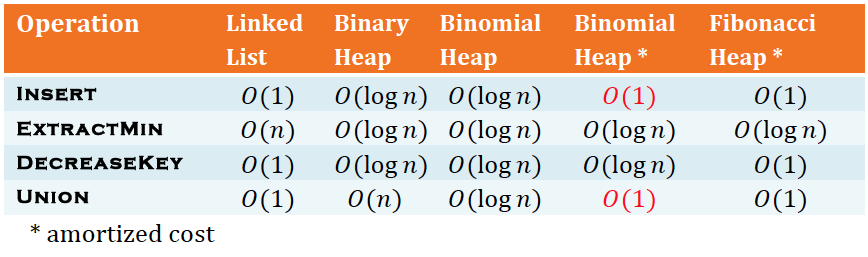
\includegraphics[width=4in]{L7-heaptablefibonacciheap.png} 
%	\end{center}
%\end{figure}

\begin{table}[!ht]
\centering
\begin{tabular}{ p{2.4cm}p{1.1cm}p{1.3cm}p{1.4cm}p{1.4cm}p{1.5cm} }
\hline
 \textcolor{blue}{\textbf{Operation}} & \textcolor{blue}{\textbf{Linked List}}  & \textcolor{blue}{\textbf{Binary Heap}} & \textcolor{blue}{\textbf{Binomial Heap}} & \textcolor{blue}{\textbf{Binomial Heap*}} & \textcolor{blue}{\textbf{Fibonacci Heap*}}\\
 \hline
 {\sc Insert} & $O(1)$ & $O(\log n)$ & $O(\log n)$  & \textcolor{red}{$O(1)$} & $O(1)$\\
 {\sc ExtractMin} & $O(n)$ & $O(\log n)$ & $O(\log n)$ & $O(\log n)$ & $O(\log n)$\\
 {\sc DecreaseKey} & $O(1)$ & $O(\log n)$ & $O(\log n)$ & $O(\log n)$ & $O(1)$\\
 {\sc Union} & $O(1)$ & $O(n)$ & $O(\log n)$ & \textcolor{red}{$O(1)$} & $O(1)$\\
 \hline
\end{tabular}
\end{table}
*amortized cost
}



\frame{
	\frametitle{ Time complexity of {\sc Dijkstra} algorithm} 

  \begin{table}
  \begin{tabular}{crrrr}
  \hline  \hline
  Operation & Linked  & Binary  & Binomial  & Fibonacci  \\
            &  list &  heap &  heap & heap \\
  \hline
  {\sc MakeHeap} & $ 1 $ &  $1$  & $ 1 $ & $1$  \\ 
  {\sc Insert} & $ 1 $ &  $\log n$  & $ \log n $ & $1$  \\ 
   {\sc ExtractMin} & $ n $ &  $\log n$  & $ \log n  $ & $ \log n $  \\ 
  {\sc DecreaseKey} & $ 1 $ &  $\log n$  & $ \log n $ & $1$  \\ 
  {\sc Delete} & $ n $ &  $\log n$  & $ \log n $ & $\log n$  \\ 
  {\sc Union} & $ 1 $ &  $ n $  & $ \log n $ & $1$  \\ 
   {\sc FindMin} & $ n $ &  $1$  & $ \log n $ & $1$  \\ 
  \hline 
  {\sc Dijkstra} & $ O(n^2) $ &  $ O(m \log n) $  & $ O( m \log n ) $ & $ O( m + n \log n) $  \\ 
  \hline \hline 
  \end{tabular} 
  \end{table}
{\sc Dijkstra} algorithm: $n$ {\sc Insert}, $n$ {\sc ExtractMin}, and $m$ {\sc DecreaseKey}. 
}


\end{document}
